\documentclass[conference]{IEEEtran}
\usepackage[T1]{fontenc}
\usepackage{placeins}
\usepackage{amsmath,amssymb,graphicx,booktabs,array,longtable,url,hyperref}
\hypersetup{hidelinks,pdftitle={TraceMemory: Spatial Source Correction and Memory for Rectified-Flow Image Editing}}
\newcommand{\RMS}{\operatorname{RMS}}
\newcommand{\softmax}{\operatorname{softmax}}
\newcommand{\clip}{\operatorname{clip}}
\newcommand{\E}{\mathbb{E}}
\newcommand{\ind}{\mathbb{1}}
\title{TraceMemory: Spatial Source Correction and Memory for Rectified-Flow Image Editing}
\author{}
% Extended research manuscript. Main text, references, and full appendices.
% Saved experiment snapshots are retained as provenance, not rewritten as new runs.
\begin{document}
\raggedbottom
\setcounter{topnumber}{3}
\setcounter{dbltopnumber}{3}
\renewcommand{\topfraction}{0.95}
\renewcommand{\dbltopfraction}{0.95}
\renewcommand{\textfraction}{0.05}
\renewcommand{\floatpagefraction}{0.75}
\renewcommand{\dblfloatpagefraction}{0.75}
\maketitle
\begin{abstract}
Text-guided image editing couples requested changes with preservation of unaffected content. TraceMemory separates three interventions in a frozen rectified-flow editor: correction magnitude, request-conditioned spatial allocation, and source-attention coverage. Native prompt-response probes estimate protection support, and a direct local update applies the residual without global RMS restoration. We derive the support-energy relation and construct a global control with equal correction RMS at any common state. On 40 independent PIE-Bench sources with 520 outputs, local routing reduces preservation-region LPIPS by 0.0084 (95\% source-bootstrap interval $[-0.0143,-0.0022]$) and full-image LPIPS by 0.0064 relative to this control. A ten-source dose study shows monotonically improved preservation across coefficients 0.15, 0.25, and 0.35. Gating source memory by request support increases directional CLIP by 0.0207 while increasing preservation LPIPS by 0.0127. These controlled results distinguish a localization benefit from dose-dependent retention and the semantic--preservation trade-off introduced by memory release. The primary configuration uses 97 transformer evaluations, with component and external comparisons reported under source-level statistical analysis.
\end{abstract}
\begin{IEEEkeywords}
image editing, rectified flow, source memory, spatial correction, residual normalization
\end{IEEEkeywords}

\section{Introduction}
Text-guided editing should realize a requested change while retaining the source attributes that the request leaves intact. A musical-note mug should remain recognizable in a moonlit scene, and a studio portrait should retain the person's identity and shirt graphics. Other requests deliberately change material, pose, or category. The intended edit therefore determines which source properties deserve protection. Figure~\ref{fig:motivation} illustrates the scene-change and detail-retention objectives.

Inversion and source-feature reuse provide useful reference information. Their combination introduces a less visible design choice: a spatial mask selects the support of a correction, while a normalization rule sets the magnitude delivered through that support. Matching a numerical coefficient does not match the applied magnitude. Matching a global RMS can instead concentrate the same magnitude into fewer locations. Source memory further changes the edited trajectory on which subsequent residuals are evaluated. A controlled comparison must distinguish these effects before attributing an outcome to localization.

\begin{figure*}[t]
\centering
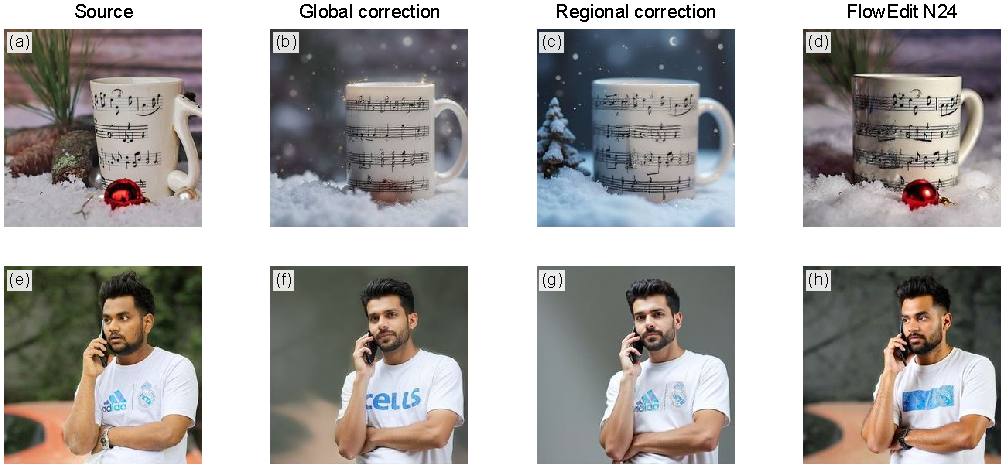
\includegraphics[width=.98\textwidth,height=.72\textheight,keepaspectratio]{figures/motivation.pdf}
\caption{Motivating examples from the spatial-allocation study. Regional correction is the unfiltered ROI\_UNIFORM25 control; global correction is U25\_KV. The mug uses seed 10 and the printed shirt seed 17. Each comparison uses the same source and target prompt. Regional allocation retains more source-like details in these examples. FlowEdit N24 illustrates a source-preserving operating point with weaker visible scene change. Exact geometry and scene attributes are examined separately in the failure analysis.}
\label{fig:motivation}
\end{figure*}

TraceMemory evaluates this interaction in a frozen rectified-flow model. A fixed source reference defines path velocity; a source-conditioned evaluation at the current edited state supplies the correction residual. The primary configuration, TraceMemory (CORR25; archived as \texttt{RELEASE\_CORR25}), applies $0.25P\odot c_i$ with request-conditioned protection $P=1-0.75E$, full-image target generation, and full-source, all-query memory during the first seven steps. Three native prompt-response probes cost six transformer evaluations, yielding 97 standalone evaluations. ONLINE normalization is retained as a historical mechanism control. A global same-state energy control isolates spatial routing from instantaneous correction magnitude. The preregistered BOTH configuration additionally gates memory queries by protection support and remains a secondary comparison.

The contributions are:
\begin{enumerate}
\item An exact support-energy relation for regional RMS normalization, together with controlled supplied-region studies of spatial placement and local amplification. These studies connect the applied correction to both mask support and residual energy.
\item Request-conditioned direct residual routing with a same-state energy control. On 40 independent sources, routing reduces preservation-region and full-image LPIPS by 0.0084 and 0.0064 relative to global energy scaling; the ten-source dose study separately characterizes correction strength.
\item A controlled evaluation of residual routing and attention-memory release. Request-conditioned query gating increases directional CLIP by 0.0207 at a preservation-LPIPS cost of 0.0127, separating the semantic response to memory release from the retention effect of residual magnitude.
\end{enumerate}

Section~\ref{sec:method} specifies the primary method and controls. Section~\ref{sec:results} establishes the spatial-allocation and magnitude mechanisms. Section~\ref{sec:public-evaluation} evaluates support estimation, memory coverage, and correction dose on development sources. Section~\ref{sec:final-evaluation} then tests the frozen configurations on independent sources. The appendices provide full numeric records, reproduction details, and separately identified mechanism hypotheses.

\section{Related Work and Research Position}
\label{sec:related}
\subsection{Generative trajectories and reconstruction}
Diffusion models learn a denoising process, and implicit sampling exposes a deterministic trajectory suitable for inversion \cite{ho2020ddpm,song2021ddim}. Latent diffusion reduces the cost of high-resolution synthesis by operating in a learned image representation \cite{rombach2022ldm}. Flow matching and rectified flow learn continuous transport fields; transformer-based diffusion and scaled rectified-flow models provide architectures for joint image and text processing \cite{lipman2023flowmatching,liu2023rectifiedflow,peebles2023dit,esser2024sd3}. These foundations explain why a perturbation to a latent velocity or an attention output can influence several subsequent generation steps.

Real-image editing requires a useful source representation as well as a target instruction. SDEdit controls the amount of source destruction through noise injection \cite{meng2022sdedit}. Null-text inversion optimizes the unconditional embedding along a reconstruction trajectory, EDICT uses coupled transformations for invertibility, and PnP Inversion applies reconstruction offsets while separating source and target processes \cite{mokady2023nulltext,wallace2023edict,ju2024pnpinversion}. In rectified flows, RF-Inversion introduces endpoint-directed control, RF-Solver improves integration, and FireFlow reuses velocity information for efficient inversion \cite{rout2025rfinversion,wang2025rfsolver,deng2025fireflow}. TraceMemory uses a controlled source trajectory as a reference and measures the effect of adding a spatially allocated velocity residual during target generation.

\subsection{Direct flow editing and reference alignment}
FlowEdit constructs direct source-to-target transport from differences of source and target velocities evaluated along noised source and edited states \cite{kulikov2025flowedit}. CVC separates trajectory drift and semantic velocity differences; FlowAlign adds trajectory regularization; optimal-transport guidance supplies another route to source-aware flow editing \cite{li2025cvc,kim2025flowalign,lupascu2026otrf}. These methods make the evaluation state and reference construction central design choices.

DirectEdit saves adjacent inversion offsets, shifts the forward field-evaluation input, and combines source-value injection with mask-guided latent blending \cite{yang2026directedit}. SteerFlow combines reference-velocity alignment, trajectory interpolation, and adaptive masking derived from segmentation and source--target velocity differences \cite{dao2026steerflow}. Both are close comparisons for spatial source constraints. In the present method the target field remains global, while an additive correction is routed through a protection region and normalized explicitly. The experimental distinction concerns the location and magnitude of this residual and its interaction with a separate attention-memory channel.

\subsection{Attention and feature reuse}
Prompt-to-Prompt controls cross-attention to preserve spatial arrangements during prompt changes \cite{hertz2023prompttoprompt}. Plug-and-Play Diffusion Features transfers spatial features and self-attention to guide image translation \cite{tumanyan2023pnpfeatures}. MasaCtrl retrieves source keys and values using target queries, with mask-guided foreground/background retrieval for consistency \cite{cao2023masactrl}. These approaches establish attention reuse as a source-preservation mechanism.

Flow-based feature reuse differs in the features stored, the extraction state, and the receiving layers. RF-Edit shares source values; ReFlex extracts intermediate attention and residual features and adapts their injection; Stable Flow identifies influential layers for source-feature transfer; FluxSpace uses transformer features for semantic editing and localization \cite{wang2025rfsolver,kim2025reflex,avrahami2025stableflow,dalva2025fluxspace}. TraceMemory's local attention operation retains the target text contribution and the native image-attention mass while retrieving paired source image K/V. The comparison of all-query and ROI-query memory asks how coverage interacts with residual correction. This local algebraic preservation is defined at a fixed layer input; its final semantic effect is an empirical question.

\subsection{Spatial control and the meaning of a mask}
Blended Diffusion and Blended Latent Diffusion use spatial constraints to preserve image content during localized editing \cite{avrahami2022blended,avrahami2023blendedlatent}. DiffEdit infers an editing region from conditional model responses \cite{couairon2023diffedit}. GLIGEN introduces grounded spatial conditioning for generation, showing how explicit location information can control a generative model \cite{li2023gligen}. InstructPix2Pix learns instruction-conditioned editing from paired examples, while DiffusionCLIP and Imagic adapt models or representations to a requested change \cite{brooks2023instructpix2pix,kim2022diffusionclip,kawar2023imagic}. FreeDoM instead applies training-free energy guidance \cite{yu2023freedom}.

A protection mask and an edit mask serve different purposes. A shirt-print region identifies content to preserve; a studio-background edit region identifies content to change. Segment Anything and Grounding DINO provide segmentation and language-grounded detection components that can construct source-based regions \cite{kirillov2023sam,liu2024groundingdino}. Their outputs would be inputs to a future automatic protection pipeline. The experiments reported here use manual pattern regions. Their coordinates are also used by the local evaluation metric, and this annotation-assisted setting is retained explicitly throughout the results.

\subsection{Frequency, temporal allocation, and multi-turn editing}
FreqEdit injects high-frequency velocity information and compensates accumulated deviation for multi-turn editing \cite{liao2025freqedit}. Wavelet-guided semantic compensation extracts low-frequency same-state conditional differences as an auxiliary term for direct flow editing \cite{tang2026wavelet}. Multi-turn Consistent Image Editing combines control and attention adaptation across edits \cite{zhou2025multiturn}. These works motivate evaluating which quantity is filtered, where it is evaluated, and how its magnitude is controlled. Our spectral control filters the reference residual; its matched unfiltered counterpart isolates the effect of frequency shaping within the same spatial support.

\subsection{Evaluation and the specific research question}
CLIP provides image--text embeddings, and CLIPScore uses their similarity for reference-free image--text evaluation \cite{radford2021clip,hessel2021clipscore}. DINO and DINOv2 supply visual representations useful for content and structure comparisons \cite{caron2021dino,oquab2024dinov2}. LPIPS measures perceptual differences, and SSIM compares local structural information \cite{zhang2018lpips,wang2004ssim}. These measures address complementary outcomes. Exact logo characters, repeated objects, and a requested directional light require task-specific judgments in addition to embedding similarity.

Across this literature, source preservation is implemented through reconstruction, feature reuse, spatial constraints, or velocity guidance. The specific question studied here is how \emph{spatial support, applied correction magnitude, and memory-query coverage} interact within one fixed-reference editor. Matching the same coefficient does not match the injected RMS after masking, and changing attention coverage changes the trajectory on which the next residual is evaluated. The controlled studies quantify these interactions. Section~\ref{sec:extension} defines request-conditioned support. Appendix~\ref{sec:prospective-controls} separates area-aware and source-pool hypotheses from the completed experiments.

\begin{table*}[t]
\centering\small
\caption{Mechanism-level comparison of the nearest literature. This table records algorithmic relationships, not a measured performance ranking.}
\label{tab:nearest}
\begin{tabular}{p{.14\textwidth}p{.24\textwidth}p{.23\textwidth}p{.29\textwidth}}
\toprule
Method & Source constraint & Spatial / memory operation & Specific comparison for TraceMemory\\
\midrule
RF-Edit \cite{wang2025rfsolver} & Inversion trajectory and improved integration & Early source-value sharing & Source values versus paired K/V retrieval with retained target text contribution\\
MasaCtrl \cite{cao2023masactrl} & Source self-attention features & Source-pool masks and target-region combination & Full source pool with a query-output gate; correction controlled separately\\
ReFlex \cite{kim2025reflex} & Mid-inversion features & Attention and residual adaptation & Single-node cache versus seven reference captures and an explicit residual\\
DirectEdit \cite{yang2026directedit} & Adjacent inversion offsets & Input alignment, value injection, latent blending & Input alignment versus additive regional velocity correction\\
SteerFlow \cite{dao2026steerflow} & Reference alignment and interpolation & Adaptive edit masks and velocity steering & Edit-region velocity interpolation versus protection-region residual allocation\\
FlowEdit \cite{kulikov2025flowedit} & Randomly noised source states & Direct cross-state velocity differences & Inversion-free editing baseline under a shared input and evaluation protocol\\
TraceMemory & Controlled fixed trace & Regional residual plus separate paired K/V memory & Spatial support, magnitude normalization, and query coverage varied explicitly\\
\bottomrule
\end{tabular}
\end{table*}


\section{Request-Conditioned Source Correction and Memory}
\label{sec:method}
The design separates \emph{where source correction acts} from \emph{where target generation proceeds}. A protection mask routes an added residual; every spatial location still receives the target-conditioned velocity. Source memory is a second intervention inside attention. Its query coverage can be varied without changing the residual mask or its source-key pool. Figure~\ref{fig:method} shows the reference, response estimator, correction rule, and attention path.

\begin{figure*}[t]
\centering
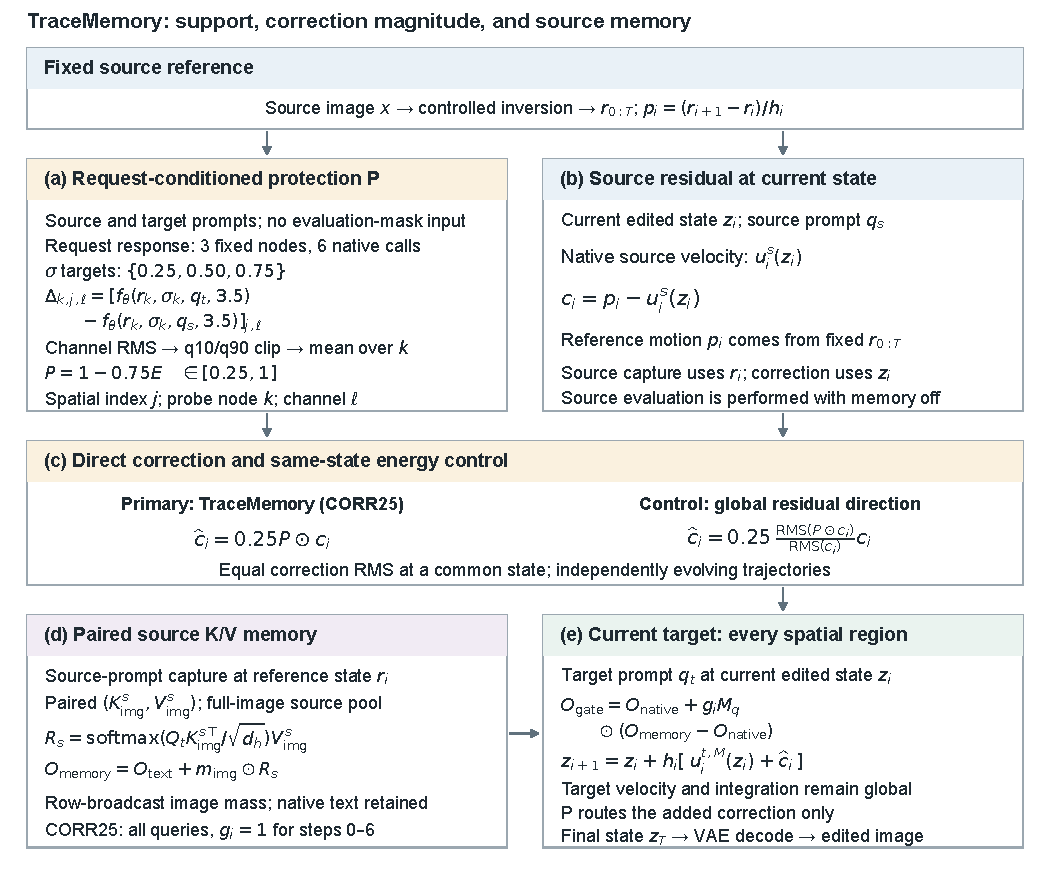
\includegraphics[width=.98\textwidth,height=.72\textheight,keepaspectratio]{figures/method_overview.pdf}
\caption{TraceMemory (CORR25) and its same-state energy control. The fixed reference supplies reference motion, native prompt-response probes, and K/V capture states. The source residual is evaluated at the current edited state. CORR25 applies direct local correction and full-source memory during the first seven steps. The control retains the global residual direction at matched instantaneous RMS. Both receive a global target-conditioned update.}
\label{fig:method}
\end{figure*}
\subsection{States and fixed source trajectory}
Let $y=\mathcal{E}_{\rm VAE}(x)$ be the source VAE latent, $q_s,q_t$ the source and target prompts, and $\mathcal{D}_{\rm VAE}(z_T)$ the decoded output. The frozen transformer predicts $f_\theta(z,\sigma,q,g)$. Generation uses decreasing scheduler nodes $\sigma_0>\cdots>\sigma_T=0$ and positive intervals $h_i=\sigma_i-\sigma_{i+1}$, with $T=28$. We write $u_i^s(z)=u_i(z;q_s)$ for the native source field and $u_i^{t,M}(z)$ for the target field with memory.
\subsection{Controlled inversion and fixed reference}
We discretize the controlled inversion ODE of RF-Inversion.\cite{rout2025rfinversion} Inversion starts from $y$ and follows the same nodes in increasing time. A seed determines one Gaussian tensor $\epsilon$. At an ascending node $t$ with positive increment $\Delta t$, the update is
\begin{equation}
w^+=w+\Delta t\left[(1-\gamma)f_\theta(w,t,\varnothing,0)+\gamma\frac{\epsilon-w}{1-t}\right].
\end{equation}
We use $\gamma=0.5$. The endpoint is reached without evaluating the denominator at $t=1$. Reversing saved states gives $r_0,\ldots,r_T$, with $r_T=y$, and editing starts at $z_0=r_0$. The reference stays fixed throughout target generation. Matched RF arms share its construction and seed.

The corresponding RF-Inversion generation controller, expressed in decreasing noise time, is\cite{rout2025rfinversion}
\begin{equation}
\begin{aligned}
u_i(z;q)&=-(1-\eta_i)f_\theta(z,\sigma_i,q,3.5)+\eta_i\frac{y-z}{\sigma_i},\\
\eta_i&=\eta_{\max}\min\left(1,\max\left(0,\frac{\sigma_i-0.2}{0.25}\right)\right).
\end{aligned}
\end{equation}
Only nodes before terminal zero are evaluated. The spatial comparisons use $\eta_{\max}=0$. Empty-prompt generation below also uses guidance 3.5, distinguishing it from inversion at guidance zero.

\subsection{Current-state source correction}
The fixed trace $r_0,\ldots,r_T$ defines reference motion. At the edited state $z_i$, define
\begin{equation}
\begin{aligned}
p_i&=(r_{i+1}-r_i)/h_i,\\
c_i&=p_i-u_i^s(z_i),\\
z_{i+1}&=z_i+h_i[u_i^{t,M}(z_i)+\widehat c_i].
\end{aligned}
\label{eq:spatial-update}
\end{equation}
Here $\widehat c_i$ is the allocated correction. Global quarter-strength correction uses $\widehat c_i=0.25c_i$. The target field remains global in every spatial arm; the ROI allocates only the added correction. At full correction and with memory disabled, the displacement from the reference evolves by the same-state target-minus-source field difference.
\subsection{Request-conditioned protection support}
\label{sec:extension}
DiffEdit estimates edit regions by comparing conditional predictions at a common noisy input. SteerFlow constructs a velocity-difference mask and combines it with a semantic segmenter \cite{couairon2023diffedit,dao2026steerflow}. These methods motivate a concrete alternative to source-only contrast. We estimate the target request's spatial response on the existing reference trajectory, before attaching source-memory hooks. Let $\mathcal K$ contain the three distinct scheduler indices closest to $\sigma\in\{0.25,0.50,0.75\}$. For spatial location $j$ and latent channel $\ell$, compute
\begin{equation}
\begin{aligned}
\Delta_k&=f_\theta(r_k,\sigma_k,q_t,3.5)-f_\theta(r_k,\sigma_k,q_s,3.5),\\
d_{k,j}&=\sqrt{\frac{1}{C}\sum_{\ell=1}^{C}[\Delta_k]_{j,\ell}^2},\qquad k\in\mathcal K.
\end{aligned}
\end{equation}
Both evaluations use the same latent, time, guidance embedding, and native network. Packed image tokens are first restored to the spatial latent grid. For each response map, let $l_k$ and $v_k$ be its spatial 10th and 90th percentiles. Define
\begin{equation}
\begin{aligned}
e_k&=\clip\!\left(\frac{d_k-l_k}{v_k-l_k},0,1\right),\\
E&=\frac{1}{3}\sum_{k\in\mathcal K}e_k,\qquad
P=0.25+0.75(1-E)=1-0.75E.
\end{aligned}
\label{eq:request-support}
\end{equation}
A degenerate percentile range contributes a zero response map and is recorded. $E$ is a relative model-response score. The support $P$ assigns a baseline correction everywhere and stronger correction to locations with lower prompt response. The primary TraceMemory (CORR25) configuration uses $P$ in Eq.~\eqref{eq:soft-support} with direct local scaling $\lambda=0.25$ and a full-image target update. The direct rule isolates local attenuation: reducing protection reduces the added correction at that location. ONLINE, used in the earlier mechanism studies, restores the global RMS after masking and therefore changes the local multiplier. Comparing the two rules motivates the final direct-local and global-energy controls. No benchmark region enters the estimator. Source K/V retrieval, target-query coverage, gate, and memory window remain unchanged.

The three source and three target probes add six transformer calls. With 28 inversion calls, 28 current-source calls, 28 target calls and seven reference-memory captures, the request-conditioned configuration costs 97 standalone NFE. The support is fixed before target generation. The probe nodes and percentile transform specify the estimator and are held fixed across its comparisons.

The exact spatial mean is $\overline{P}=1-0.75\overline{E}$, and $P_j\in[0.25,1]$. For a tensor $v$ with $N_{\rm lat}$ scalar entries, define $\RMS(v)=\sqrt{N_{\rm lat}^{-1}\sum_jv_j^2}$. Support weights broadcast across latent channels. The primary rule is $\widehat c_i^{\rm CORR}=\lambda P\odot c_i$, with $\lambda=0.25$. For comparison with historical results, the two scaling rules are
\begin{equation}
\begin{aligned}
\widehat c_i&=k_i(P\odot c_i),\\
k_i&=\begin{cases}
\lambda\RMS(c_i)/\RMS(P\odot c_i),&\text{ONLINE},\\
\lambda,&\text{LOCAL}.
\end{cases}
\end{aligned}
\label{eq:soft-support}
\end{equation}
The expression assumes nonzero supported residual; zero correction is handled explicitly. The contrast-support ablation replaces $P$ with $R_\zeta=\zeta+(1-\zeta)R$, where $R$ is a source-only contrast mask, and tests $\zeta\in\{0.25,0.50,0.75\}$. The endpoints $\zeta=0$ and $\zeta=1$ recover contrast-only support and global correction. Supplied-region controls instead use $P=M$ for an annotated protection region.

Figure~\ref{fig:request-support-map} shows the estimator's recorded response and protection maps alongside the source and resulting edit.
\begin{figure*}[t]
\centering
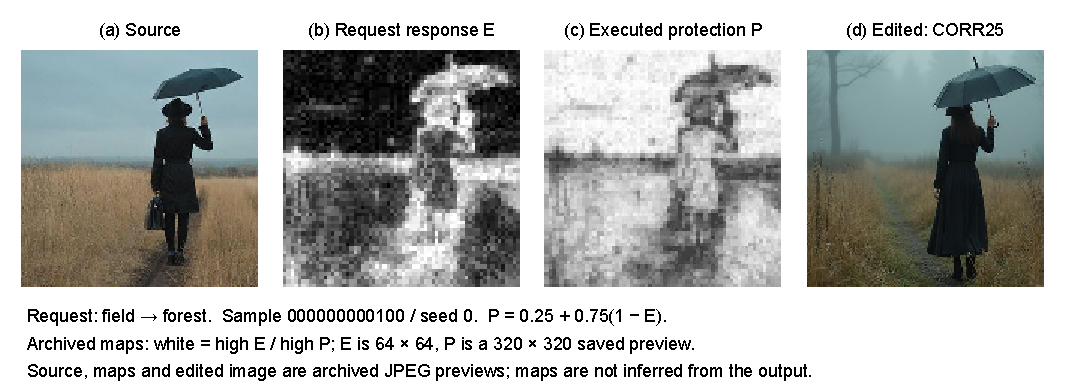
\includegraphics[width=\textwidth]{figures/figrequest_support.pdf}
\caption{Recorded request-conditioned support for a field-to-forest request. The three native source/target probes produce the response $E$; $P=1-0.75E$ defines protection before target generation. The maps are archived estimator outputs, shown with their original grayscale range.}
\label{fig:request-support-map}
\end{figure*}

\paragraph{Global same-state energy control.}
ENERGY\_MATCH25 uses
\begin{equation}
\widehat c_i^{\rm ENERGY}=0.25\frac{\RMS(P\odot c_i)}{\RMS(c_i)}c_i.
\label{eq:energy-control}
\end{equation}
At any common state this global-direction correction has the same RMS as $0.25P\odot c_i$. Each arm evaluates its residual on its own evolving state, so this construction matches the rule at the same state and step, not cumulative energy across trajectories. A zero residual gives zero correction. CORR and ENERGY share probes, source memory, schedule, and 97-NFE accounting.

\subsection{Paired source memory within the target attention budget}
For each attention head, let $Q_t\in\mathbb R^{N_q\times d_h}$ contain target image queries; $K_{\rm text}^t,K_{\rm img}^t,V_{\rm text}^t,V_{\rm img}^t$ contain native target keys and values. Native joint attention is
\begin{equation}
\begin{aligned}
A&=\softmax\left(\frac{Q_t[K_{\rm text}^t;K_{\rm img}^t]^\top}{\sqrt{d_h}}\right),\\
O_{\rm text}&=A_{\rm text}V_{\rm text}^t,\quad O_{\rm img}=A_{\rm img}V_{\rm img}^t.
\end{aligned}
\end{equation}
Here $m_{{\rm img},q}=\sum_{j\in{\rm img}}A_{qj}$ is the native image-attention mass of query $q$. Source keys and values $(K_{\rm img}^s,V_{\rm img}^s)$ are captured together during the source-prompt call at $r_i$. Define
\begin{equation}
\begin{aligned}
R_s&=\softmax\left(Q_t(K_{\rm img}^s)^\top/\sqrt{d_h}\right)V_{\rm img}^s,\\
O_{\rm native}&=O_{\rm text}+O_{\rm img},\\
O_{\rm memory}&=O_{\rm text}+m_{\rm img}\odot R_s,\\
O_{\rm gate}&=O_{\rm native}+g_iM_q\odot(O_{\rm memory}-O_{\rm native}).
\end{aligned}
\label{eq:query-gate}
\end{equation}
Both $m_{\rm img}$ and $M_q$ have shape $N_q\times1$; $\odot$ broadcasts them along the $d_h$ feature dimension. This update preserves the native text contribution and total image-attention mass at the modified layer. Text-query outputs retain their native attention. Modified image features subsequently propagate to later layers. Captured keys include key normalization and rotary position encoding.

Memory-enabled configurations use $g_i=1$ at steps 0--6 in zero-based single-stream blocks 1--26, followed by native attention. The source call captures paired K/V without modifying its output. All-query memory sets $M_q=1$; spatial-query controls average their protection support over each packed $2\times2$ latent patch. Each selected query reads the full source image-token pool. Memory-off sets $g_i=0$.
\subsection{Spatial allocation and correction magnitude}
For the supplied-region controls, let $M\in[0,1]$ be the annotated source-pattern mask and $L$ a replicate-padded $5\times5$ spatial averaging filter. On the unpacked latent grid, the spectral and unfiltered candidates are
\begin{equation}
\begin{aligned}
s_i^{\rm route}&=0.5L(c_i)+M\odot[c_i-L(c_i)],\\
s_i^{\rm ROI}&=M\odot c_i.
\end{aligned}
\label{eq:candidates}
\end{equation}
The spectral arm retains global low-frequency correction and routes its high-frequency component through $M$. ROI\_UNIFORM25 applies no frequency filter: it restricts the entire residual to $M$ before normalization.

A completed global U25\_KV run supplies
\begin{equation}
\begin{aligned}
b_i^{\rm ref}&=\RMS(0.25c_i^{\rm U25}),\\
\widehat c_i&=b_i^{\rm ref}\,s_i/\RMS(s_i).
\end{aligned}
\label{eq:normalization}
\end{equation}
Thus ROI\_UNIFORM25 matches the global U25 per-step RMS, rather than applying the unnormalized update $0.25M\odot c_i$. The development study also evaluates the direct local coefficient below. A zero budget gives zero correction; a nonzero budget with zero candidate is an explicit failure. The realized budget is $\sum_i h_i\RMS(\widehat c_i)$.

Masks use supplied fixed pattern-region annotations, feathered inward over 16 pixels at the 512-pixel image scale, area-downsampled to the latent grid, replicated across channels, and packed for FLUX. All magnitude/coverage-study configurations use the manual \texttt{fixed\_pattern\_roi} annotation. The same annotated region defines the local pattern metric, so the comparison directly tests annotation-assisted allocation. CENTER uses one fixed center box; SHIFT moves the source ROI to the farthest available border without wrapping.

The spectral ROUTE\_ONLINE25 control uses a same-state budget $0.25\RMS(c_i)$ for its filtered candidate. The unfiltered magnitude/coverage comparison sets $P=M$ and $\lambda=0.25$ in Eq.~\eqref{eq:soft-support}. ONLINE rescales the supported residual to the current global quarter-strength RMS, while LOCAL directly applies $0.25M\odot c_i$. Both operate without a separate reference run. We record the integrated injected magnitude $I=\sum_i h_i\RMS(\widehat c_i)$.

\subsection{Exact support-energy coupling and the area approximation}
For $N_{\rm lat}$ scalar latent entries, define the retained energy fraction and squared support mass as
\begin{equation}
 e_i(P)=\frac{\sum_j P_j^2c_{i,j}^2}{\sum_j c_{i,j}^2},\qquad
 f_P=\frac{1}{N_{\rm lat}}\sum_jP_j^2.
\label{eq:support-energy}
\end{equation}
\textbf{Proposition 1 (support--energy coupling).} For a nonzero global and supported residual, ONLINE applies the exact scalar multiplier
\begin{equation}
 k_i^{\rm ONLINE}=\frac{\lambda\RMS(c_i)}{\RMS(P\odot c_i)}=\frac{\lambda}{\sqrt{e_i(P)}},
 \qquad k_i^{\rm LOCAL}=\lambda.
\label{eq:exact-multiplier}
\end{equation}
\emph{Proof.} Squaring the ratio of supported to global RMS cancels the common number of latent entries and gives $e_i(P)$. Substitution into the normalization rule yields Eq.~\eqref{eq:exact-multiplier}. For $0\leq P_j\leq1$, the supported residual norm is at most the global norm, so $k_i^{\rm ONLINE}\geq\lambda$. A uniform support $P_j=a>0$ gives $e_i(P)=a^2$ and $k_i^{\rm ONLINE}=\lambda/a$.\hfill$\square$

Thus concentrating global RMS through a mask changes local amplitude. If residual squared magnitude is spatially uniform, or uncorrelated with squared support, then $e_i(P)\simeq f_P$. For a binary mask of area fraction $f$, this gives $k_i^{\rm ONLINE}\simeq \lambda/\sqrt f$. For a texture-selective or request-dependent support, measured $e_i(P)$ captures the additional energy correlation. The spatial mean of a nonuniform support does not determine this energy-weighted multiplier.

The integrated injected RMS, $I=\sum_i h_i\RMS(\widehat c_i)$, records intervention magnitude. Vector cancellation, nonlinear field evolution, and memory changes determine the resulting displacement. This distinction separates a controlled injection measurement from output retention and requested-edit achievement. The completed ONLINE/LOCAL contrast tests the difference between two implemented scaling rules. Area-exponent interpolation and amplitude caps are specified separately in Appendix~\ref{sec:prospective-controls} as hypotheses.

\subsection{Reference following and edit displacement}
For full correction without memory, define $\delta_i=z_i-r_i$. Substituting $\widehat c_i=p_i-u_i^s(z_i)$ gives
\begin{equation}
\delta_{i+1}=\delta_i+h_i\{u_i(z_i;q_t)-u_i(z_i;q_s)\}.
\label{eq:displacement}
\end{equation}
With identical prompts, identical field computation, and $z_i=r_i$, this yields $z_{i+1}=r_{i+1}$. With different prompts, departure depends on the conditional velocity difference. This identity describes a mechanism for weak departure when the difference is small. The size and direction of that difference must be measured for each editing configuration. The residual also contains effects of the inversion controller and conditioning choices; its interpretation extends beyond Euler truncation error.

\begin{table}[t]
\centering\small
\caption{Algorithm 1: Primary TraceMemory (CORR25) update and explicit controls. Source-reference capture and current-state source evaluation are distinct calls.}
\label{alg:ours}
\begin{tabular}{p{.94\columnwidth}}
\toprule
\textbf{Inputs:} source $x$, prompts $q_s,q_t$, seed, nodes $\sigma_i$, coefficient $\lambda=0.25$.\\
1. Encode $y=\mathcal{E}_{\rm VAE}(x)$; build reference $r_{0:T}$; set $z=r_0$. Compute $P=1-0.75E$ by Eq.~\eqref{eq:request-support} using six native calls.\\
2. For each generation step $i=0,\ldots,T-1$:\\
\quad Compute $p_i=(r_{i+1}-r_i)/h_i$.\\
\quad If $i<7$, capture source K/V from $r_i$ under $q_s$.\\
\quad Evaluate native source field $u_i^s(z)$ and target field $u_i^{t,M}(z)$.\\
\quad Form $c_i=p_i-u_i^s(z)$ and $s_i=P\odot c_i$.\\
\quad Primary CORR: set $\widehat c_i=0.25s_i$ directly.\\
\quad ENERGY control: use Eq.~\eqref{eq:energy-control}. Historical ONLINE: $\widehat c_i=0.25\RMS(c_i)s_i/\RMS(s_i)$.\\
\quad Update $z\leftarrow z+h_i(u_i^{t,M}(z)+\widehat c_i)$; record norms and calls.\\
3. Decode $\mathcal{D}_{\rm VAE}(z)$; save the image and its task/seed/parameter record.\\
\bottomrule
\end{tabular}
\end{table}

\section{Controlled Spatial Allocation and Magnitude Mechanisms}
\label{sec:results}
\subsection{Design, inputs, and configuration}
The spatial-allocation study contains 98 outputs: seven configurations, seven tasks, and two seeds. The magnitude/coverage study contains 70 outputs: five configurations on the same task--seed pairs. Both studies use six independent source images. Dog/rain and dog/snow share one source image and remain in the same statistical cluster. Cup/night uses seeds 10 and 17; the other tasks use seeds 0 and 17. The complete tasks are cup/night, printed-shirt/studio, butterfly/sunset, plain-shirt/studio, dog/snow, dog/rain, and rug/wooden-floor.

All methods in these tables use FLUX.1-dev at $512\times512$. The transformer uses BF16, integration uses FP32, and source encoding uses the VAE posterior mode. The RF branches use 28 inversion and 28 generation intervals. FlowEdit N24 uses 28 scheduler nodes, $n_{\max}=24$, $n_{\min}=0$, one noise sample, and source/target guidance 1.5/5.5. It is the external configuration measured within the spatial-allocation study. Frozen N26 reference images in the full sheets retain their own configuration labels and are excluded from the new-output counts.

The evaluated TraceMemory masks are manual fixed-pattern regions with 16-pixel inward feathering. They are reused as local evaluation support. This defines an annotation-assisted comparison. The center and shifted controls vary routing support while retaining the original evaluation region. Complete prompts, ROI coordinates, model revision, and task mappings appear in Appendix~\ref{sec:evidence-appendix}.

\subsection{Outcomes and evidence scope}
The tables use metrics recorded from lossless output PNGs and source evaluation PNGs, evaluated at 512 pixels. For $N_{\rm pix}$ RGB pixels, source departure is
\begin{equation}
\operatorname{MAE}=\frac{1}{3N_{\rm pix}}\sum_{j=1}^{N_{\rm pix}}\sum_{\ell=1}^{3}|x_{j,\ell}-\widehat x_{j,\ell}|.
\end{equation}
Its direction is task-dependent because a requested background change also changes pixels. For grayscale source and output crops $a,b$, normalized cross-correlation is
\begin{equation}
\operatorname{NCC}(a,b)=\frac{\langle a-\bar a,b-\bar b\rangle}{\|a-\bar a\|_2\|b-\bar b\|_2}.
\end{equation}
Grayscale weights are $(0.2126,0.7152,0.0722)$. Fixed NCC compares the same annotated box. NCC$_{\pm6}$ takes the largest valid correlation over all integer output-crop shifts in $[-6,6]^2$, favoring the smallest displacement when tied. Flat crops have undefined correlation and are reported as missing. Both fixed and shifted results are retained so that tolerance to small displacement is visible.

Tables quantify native-image retention and departure; visual comparisons identify task-specific edits and artifacts. Joint edit--preservation assessment follows Appendix~\ref{sec:review-protocol}; evaluation coverage is recorded in Appendix~\ref{sec:evaluation-provenance}.

\subsection{Spatial allocation at a matched correction magnitude}
Table~\ref{tab:r78} compares residual support and filtering at the global U25 per-step RMS target. Spectral routing increases mean NCC$_{\pm6}$ from 0.4901 to 0.6521, while whole-image MAE changes from 0.1053 to 0.1073. Every paired task--seed observation improves local NCC. The matched design isolates the allocation of the injected residual magnitude within the implemented system.

Correctly located routing exceeds shifted routing by 0.2423 mean NCC (Fig.~\ref{fig:mask-position}). The shifted mask preserves its size and moves to a distant border, with the correction RMS matched to the same reference profile. This measures the importance of placing a protection constraint at the evaluated pattern. The contrast is an annotation-assisted localization intervention; automatic contrast-region results are reported in Section~\ref{sec:independent}.

\begin{figure*}[t]
\centering
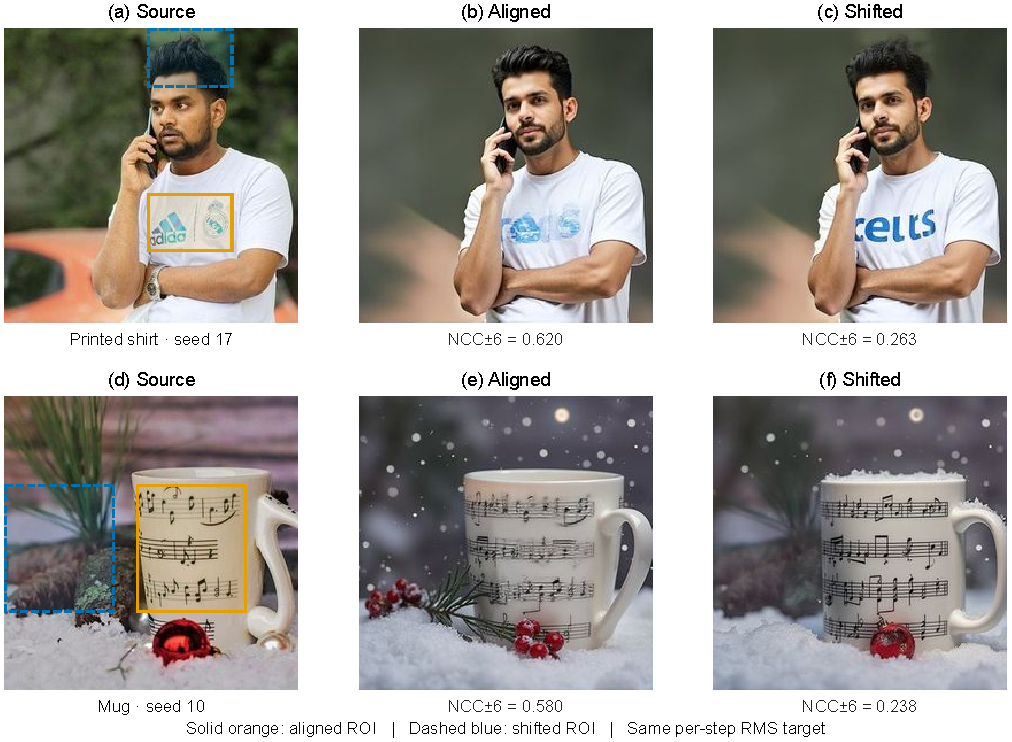
\includegraphics[width=.97\textwidth,height=.72\textheight,keepaspectratio]{figures/mask_position.pdf}
\caption{A controlled change in routing position. Solid orange and dashed blue boxes show the actual aligned and shifted routing supports on each source image. Output labels give the individual image NCC values; output panels preserve the original generated previews. The printed shirt uses seed 17 and the mug seed 10. Correct and shifted arms share the same per-step RMS target and source memory. The local metric remains anchored to the original source-pattern region.}
\label{fig:mask-position}
\end{figure*}

Unfiltered regional correction further increases NCC$_{\pm6}$ to 0.7496, a gain of 0.0975 over spectral routing and an increase in every pair. Its whole-image MAE rises to 0.1554. In this comparison, stronger local source correlation coexists with greater global source departure. The global low-frequency component of the spectral arm is therefore a meaningful control, and the unfiltered arm provides the simpler retention-oriented candidate.

The spectral online control reaches NCC$_{\pm6}$ 0.6416 compared with 0.6521 for external-profile normalization. It removes the prerequisite U25 generation and reduces standalone cost from 182 to 91 model calls. Both variants use the same manual mask rule.
\begin{table*}[t]
\centering\small
\caption{Spatial-allocation study: 14 task--seed outputs per arm. Fixed NCC uses the annotated pattern region; NCC$_{\pm6}$ permits a displacement search of up to six pixels. Costs include inversion. Required NFE also charges the prerequisite 91-call U25 run.}
\label{tab:r78}
\begin{tabular}{lrrrrr}
\toprule
Configuration & Source MAE & Fixed NCC $\uparrow$ & NCC$_{\pm6}$ $\uparrow$ & Branch NFE & Required NFE\\
\midrule
U25\_KV & 0.1053 & 0.4799 & 0.4901 & 91 & 91\\
ROUTE25 & 0.1073 & 0.6469 & 0.6521 & 91 & 182\\
ROI\_UNIFORM25 & 0.1554 & 0.7479 & 0.7496 & 91 & 182\\
ROUTE\_CENTER25 & 0.1126 & 0.5506 & 0.5542 & 91 & 182\\
ROUTE\_SHIFT25 & 0.1054 & 0.3923 & 0.4098 & 91 & 182\\
ROUTE\_ONLINE25 & 0.1083 & 0.6369 & 0.6416 & 91 & 91\\
FLOWEDIT\_N24 & 0.0757 & 0.7322 & 0.7339 & 48 & 48\\
\bottomrule
\end{tabular}
\end{table*}
\subsection{Online magnitude and attention coverage}
Table~\ref{tab:r79} evaluates the unfiltered residual under two magnitude rules and two memory-query supports. The historical label Ours--ONLINE denotes ONLINE/all, matching the released ROI\_ONLINE25 arm; the current primary method is TraceMemory (CORR25). Figure~\ref{fig:r79-main} labels this candidate explicitly beside its controls.

With all-query memory, ONLINE increases NCC$_{\pm6}$ from 0.4445 to 0.7864 in all 14 paired outputs. Its mean correction impulse is 0.2524, compared with 0.0921 for LOCAL. The observed 2.74-fold increase in impulse is central to interpretation: these two rules produce different effective correction strengths despite sharing the coefficient 0.25.

Restricting ONLINE memory to ROI queries increases source MAE in all pairs, from 0.1543 to 0.2350. Its local NCC rises in eight pairs and falls in six, with mean difference $-0.0272$. The largest task-average decreases occur on the plain and printed shirts. The same query restriction under LOCAL increases MAE in every pair and reduces NCC in 10 of 14 pairs. Attention coverage also changes the evolving residual, increasing ONLINE mean impulse from 0.2524 to 0.3046. Query coverage and effective correction therefore need a joint, magnitude-controlled comparison.

Under LOCAL, all-query memory increases mean local NCC from 0.1674 to 0.4445 and reduces MAE in every pair. NCC improves in 12 of 14 pairs; the two rug outputs are exceptions. This result supports source memory in most examples of this local-coefficient setting and identifies repeated pattern structure as a concrete failure case for retrieval.

\begin{figure*}[t]
\centering
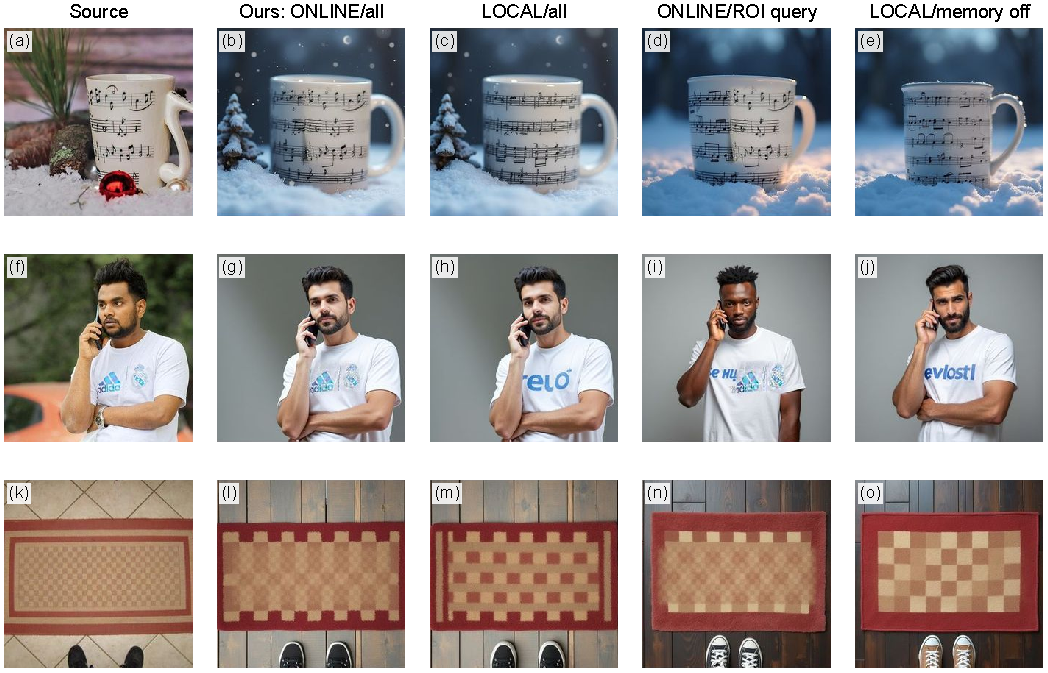
\includegraphics[width=.99\textwidth,height=.72\textheight,keepaspectratio]{figures/r79_main.pdf}
\caption{Supplied-region configuration and controls: mug/night seed 10, printed-shirt/studio seed 17, and rug/floor seed 17. \textbf{Historical Ours: ONLINE/all} is the historical ROI\_ONLINE25 configuration with a supplied pattern ROI. LOCAL/all changes the magnitude rule; ONLINE/ROI query changes memory coverage; LOCAL/memory off disables memory at the local coefficient. All panels are recorded outputs. Full sheets for both seeds and every task appear in the appendix.}
\label{fig:r79-main}
\end{figure*}

\begin{table*}[t]
\centering\small
\caption{Magnitude/coverage study: 14 outputs per configuration. All masks are manual fixed-pattern ROIs. $I$ is realized correction impulse; the budget rules produce different applied magnitudes. NFE includes inversion and requires no external budget run. ONLINE/all is the supplied-region configuration; rows are grouped by intervention, not ranked by overall editing quality.}
\label{tab:r79}
\begin{tabular}{llrrrrr}
\toprule
Correction & Memory queries & Source MAE & Fixed NCC $\uparrow$ & NCC$_{\pm6}$ $\uparrow$ & $I$ & NFE\\
\midrule
ONLINE & All & 0.1543 & 0.7857 & 0.7864 & 0.2524 & 91\\
ONLINE & ROI & 0.2350 & 0.7538 & 0.7592 & 0.3046 & 91\\
LOCAL & All & 0.1645 & 0.4319 & 0.4445 & 0.0921 & 91\\
LOCAL & ROI & 0.2481 & 0.3164 & 0.3473 & 0.0945 & 91\\
LOCAL & Off & 0.2573 & 0.1478 & 0.1674 & 0.1015 & 84\\
\bottomrule
\end{tabular}
\end{table*}
\subsection{Paired estimates and uncertainty}
We pair outputs by source, task, and seed. Table~\ref{tab:paired} reports task-weighted mean differences, with a source-cluster bootstrap that keeps both dog tasks and all seeds together. Each interval uses 100,000 resamples of six source clusters. Source-weighted estimates, exact source sign-flip values, full numeric records, and the deterministic resampling seed appear in Appendix~\ref{sec:evidence-appendix}. The contrasts are descriptive analyses of the development data; intervals capture variation among these source clusters. Figure~\ref{fig:paired} summarizes the paired effects, and Fig.~\ref{fig:departure} separates local correlation from background source departure.

\begin{table}[t]
\centering\footnotesize
\setlength{\tabcolsep}{3pt}
\caption{Selected paired local-NCC contrasts. Positive values favor the first configuration. Each row contains 14 task--seed pairs from six source clusters. Different rows answer different intervention questions; ONLINE versus LOCAL changes correction magnitude.}
\label{tab:paired}
\begin{tabular}{p{.43\columnwidth}rr}
\toprule
Contrast & Difference & 95\% interval\\
\midrule
Spectral ROI $-$ global U25 & +0.162 & [0.096, 0.244]\\
Unfiltered ROI $-$ spectral ROI & +0.097 & [0.049, 0.160]\\
Correct ROI $-$ shifted ROI & +0.242 & [0.162, 0.344]\\
ONLINE/all $-$ LOCAL/all & +0.342 & [0.224, 0.482]\\
ONLINE/ROI query $-$ ONLINE/all & $-0.027$ & [$-0.090$, 0.021]\\
LOCAL/all $-$ LOCAL/off & +0.277 & [0.103, 0.410]\\
\bottomrule
\end{tabular}
\end{table}

\begin{figure}[!t]
\centering
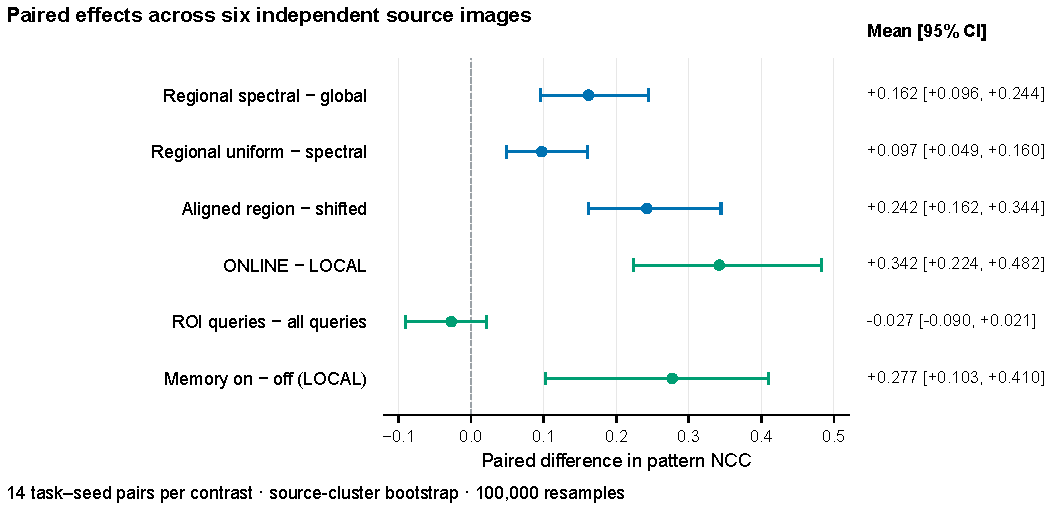
\includegraphics[width=\columnwidth]{figures/paired_summary.pdf}
\caption{Paired pattern-retention effects for six selected contrasts. Points give task-weighted mean differences; bars give 95\% source-cluster bootstrap intervals. Blue denotes spatial-allocation contrasts and green denotes magnitude/coverage contrasts. Each contrast contains 14 task--seed pairs from six independent source images; dog/rain and dog/snow are resampled together.}
\label{fig:paired}
\end{figure}

\begin{figure*}[t]
\centering
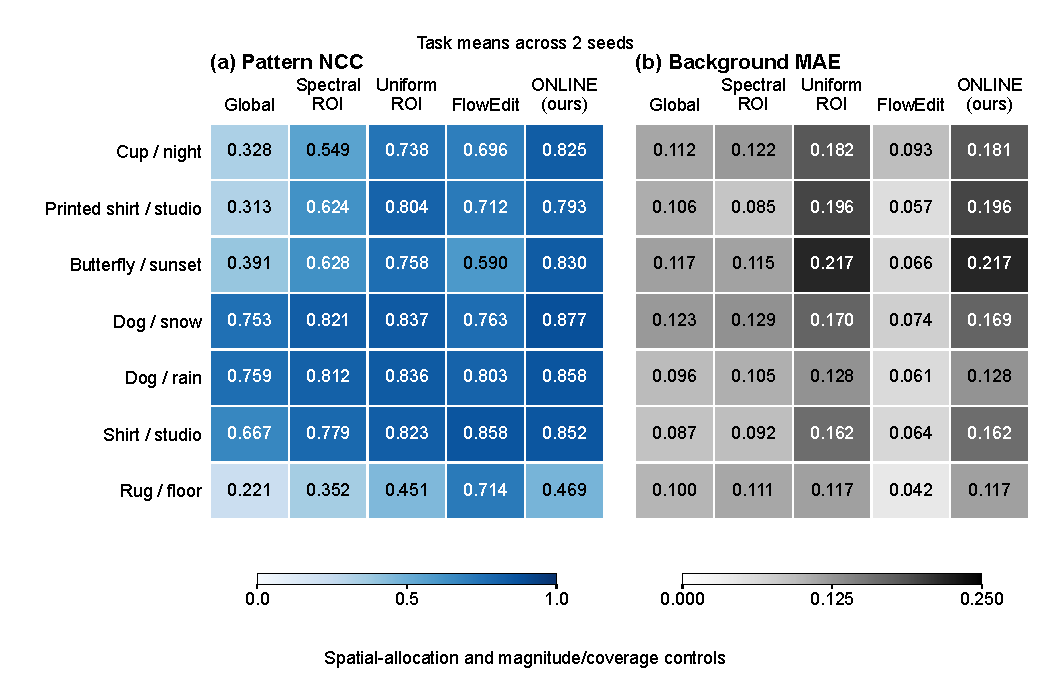
\includegraphics[width=.92\textwidth,height=.72\textheight,keepaspectratio]{figures/background_retention.pdf}
\caption{Task-level pattern retention and background source deviation. Each cell averages two seeds. Blue encodes pattern NCC and gray encodes background MAE, with independently labeled scales. The first four configurations come from the spatial-allocation study; ONLINE comes from the magnitude/coverage study. Background MAE measures the amount of change; semantic edit achievement is evaluated separately.}
\label{fig:departure}
\end{figure*}

\subsection{Computational cost}
In the historical supplied-region study, every memory-enabled ONLINE or LOCAL output uses 91 transformer evaluations: 28 for inversion, 28 for the current-state source field, 28 for target generation, and seven fixed-reference source captures. Memory-off uses 84. FlowEdit N24 uses 48 without inversion. Thus the historical Ours--ONLINE configuration uses about 1.90 times the standalone transformer-call count of this FlowEdit setting. Detector/segmenter computation is absent from the measured manual-ROI runs.

External-profile arms require both U25 and the dependent branch, giving $91+91=182$ calls for a fresh result. A shared profile can serve multiple branches; for $K$ branches charge $91+91K$, or $28+63(K+1)$ when the inversion is explicitly reused. Appendix~\ref{sec:evidence-appendix} reports recorded wall-clock values by arm and task. Model loading, transfer, and first-use effects are included where the logs include them, so those times describe the recorded execution rather than a dedicated latency benchmark.

\section{Support Estimation, Memory Coverage, and Dose on Development Sources}
\label{sec:public-evaluation}
\subsection{Source-Disjoint Pilot and Parameter Sensitivity}
\label{sec:independent}
\subsubsection{A source-disjoint pilot and a separate development sweep}
Tables report source-referenced pixel measurements; evaluation provenance is documented in Appendix~\ref{app:evaluation-provenance}.

We evaluate five methods on 24 PIE-Bench sources with two seed slots per source. Selection used a fixed SHA256 ranking and category round-robin rule, excluding the six historical development sources; the first four categories contribute three sources each and the other six two each. The pilot sources subsequently inform development, including the ten-source support and memory ablations below. A separate parameter sweep uses the historical six-source, seven-task development set.

The automatic configuration, AUTO\_DETAIL, uses the same unfiltered regional update and online budget coefficient $a=0.25$ as Eq.~\eqref{eq:soft-support}. Its mask is computed solely from source-image contrast. After grayscale area resizing to the latent grid, absolute horizontal and vertical differences are summed, smoothed with a $5\times5$ average, thresholded at the image's 75th percentile, and smoothed again. This procedure selects detailed image regions. It uses neither an object segmenter nor a target instruction. Official PIE edit masks are reserved for evaluation. Memory remains active in steps 0--6 with gate one and all-image query coverage.

The four comparators are global quarter-strength correction with memory (U25\_KV), RF-Inversion with maximum $\eta=0.3$ (ETA03), FlowEdit N26, and the released RF-Edit adapter. FlowEdit uses 28 scheduler nodes, $n_{\max}=26$, $n_{\min}=0$, one noise sample, and source/target guidance 1.5/5.5. The RF-Edit adapter uses 25 second-order steps per direction, 20 injection steps, and guidance 1/5; its configuration is kept fixed across sources. It uses 100 transformer evaluations and is deterministic for these inputs. Deterministic repeats are aggregated within source; record-level details appear in the provenance appendix.

\subsubsection{Metric support and source-level inference}
The independent cohort evaluates edit-region and preservation-region MAE using the official PIE mask and its complement. Five sources have an empty preservation complement, yielding 19 sources and 38 outputs per method for preservation MAE. Edit-region MAE uses all 24 sources. Larger edit-region departure measures a larger pixel change; achievement of the requested transformation is a separate outcome.

The archived independent-cohort NCC uses the whole image. The crop spans the image boundary, so only zero displacement is valid in the shift search. Fixed and shifted NCC are consequently identical. This metric has a different support from the local pattern NCC in the development tables. Tables report those two scopes separately.

Paired differences match source, task, and seed, averaging repeated observations within source before 20,000 source-bootstrap resamples. Two-sided sign-flip tests use 20,000 draws with plus-one correction and Holm adjustment across four comparators within each metric. The intervals and tests are exploratory. The accompanying qualitative record covers all 48 pilot sheets.

\begin{table*}[t]
\centering\small
\caption{Independent-source pilot: 24 new sources and 48 output records per method. NCC is whole-image source correlation. Preservation MAE covers 19 sources with nonempty preservation masks; edit-region MAE covers all 24. Arrows apply to source retention within the named support. Edit-region departure has no quality arrow. Runtime is recorded synchronized execution time. RF-Edit values describe the released adapter and operating point.}
\label{tab:independent}
\begin{tabular}{lrrrrrr}
\toprule
Method & Whole-image NCC $\uparrow$ & Preservation MAE $\downarrow$ & Edit-region MAE & NFE & Time (s) & Outputs\\
\midrule
ETA03 & 0.6905 & 0.1135 & 0.1471 & 56 & 40.12 & 48\\
U25\_KV & 0.7464 & 0.1093 & 0.1400 & 91 & 43.67 & 48\\
AUTO\_DETAIL & 0.5995 & 0.1627 & 0.1790 & 91 & 44.29 & 48\\
FlowEdit N26 & 0.6879 & 0.1099 & 0.1615 & 52 & 31.20 & 48\\
RF-Edit adapter & 0.9814 & 0.0216 & 0.0302 & 100 & 46.69 & 48\\
\bottomrule
\end{tabular}
\end{table*}

\subsubsection{Automatic contrast routing increases unintended change}
Table~\ref{tab:independent} shows a transfer gap. AUTO\_DETAIL minus U25\_KV gives a whole-image NCC difference of $-0.14685$ and preservation-MAE difference of $+0.05338$, with source-bootstrap intervals $[-0.21115,-0.09307]$ and $[0.03767,0.06833]$. Relative to FlowEdit N26, the differences are $-0.08842$ in NCC, with interval $[-0.16775,-0.01004]$, and $+0.05278$ in preservation MAE, with interval $[0.03113,0.07455]$. Figure~\ref{fig:independent-effects} includes all four comparisons.

These results locate the problem more precisely than whole-image similarity alone: the additional departure includes pixels that the benchmark marks for preservation. The source-only contrast support also contains edges of content explicitly requested to change and leaves smooth retained content weakly constrained. This mask-selection explanation motivates the next controlled intervention; it is distinct from the measured preservation error itself.

\begin{figure*}[t]
\centering
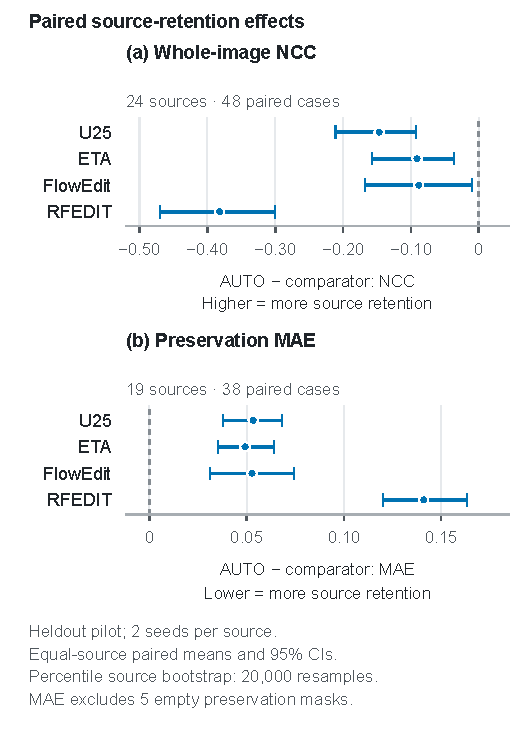
\includegraphics[width=.96\textwidth]{figures/r81_paired_effects.pdf}
\caption{AUTO\_DETAIL minus each comparator on new sources. Points are equally weighted source-level paired means; bars are percentile 95\% source-bootstrap intervals. NCC uses 24 sources; preservation MAE uses the 19 sources with nonempty preservation complements. These measurements describe source retention.}
\label{fig:independent-effects}
\end{figure*}

RF-Edit has the strongest source correlation and edit-region departure of 0.030. Its illustrated color, deletion, replacement, and style outputs remain close to the source scene. These observations characterize the recorded operating point; the adapter follows the official default injection schedule, with implementation provenance in Appendix~\ref{app:evaluation-provenance}.

\subsubsection{Visible edits and remaining semantic failures}
Figure~\ref{fig:independent-examples} presents two visible edits and two failures selected for illustration. AUTO\_DETAIL changes the kitten toward pale yellow while retaining the patterned blanket. In the deletion example, the foreground olives disappear and the pouring action remains, alongside changes to the bowl and setting. In the highway example, vehicles remain despite the request for boats. In the style example, overlapping child faces appear and the requested crayon rendering remains weak. The full per-seed observations also record changes in subject count, geometry, and surroundings. These image-specific observations explain why edit achievement, identity, preservation, and artifacts are separate evaluation dimensions.

\begin{figure*}[t]
\centering
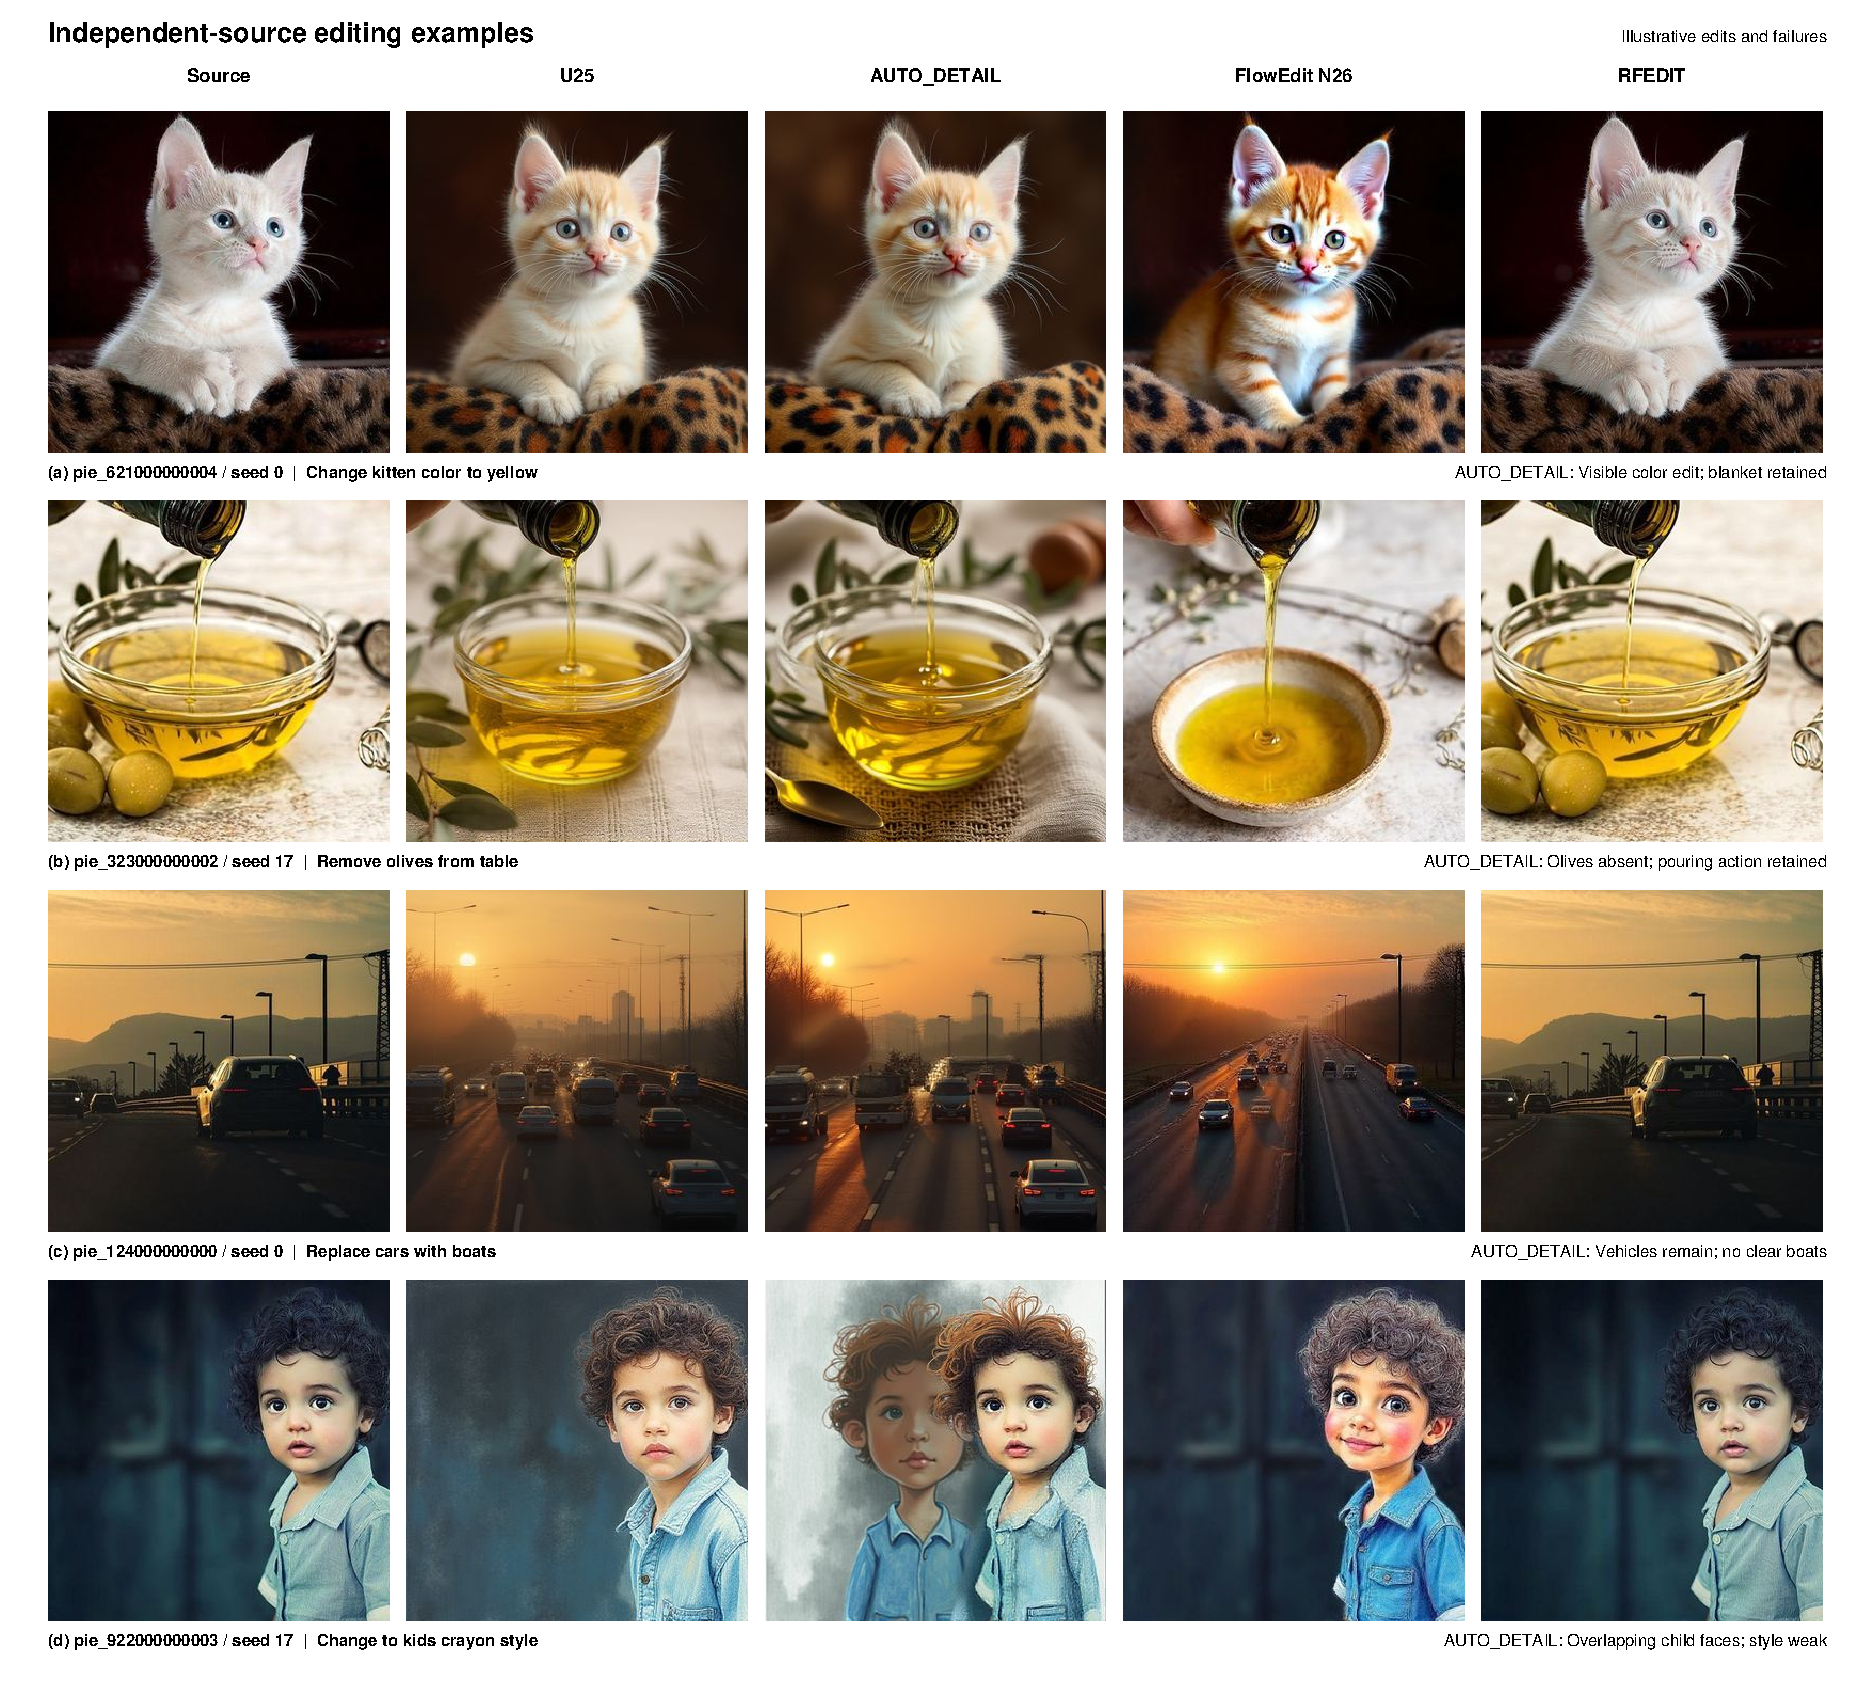
\includegraphics[width=.98\textwidth]{figures/r81_heldout_examples.pdf}
\caption{Independent-source examples with fixed prompts and seeds across methods. Rows show kitten recoloring, olive removal, car-to-boat replacement, and a crayon-style request. The first two illustrate visible requested changes with varying source retention; the last two illustrate missing replacement and duplicated geometry. Figure selection is qualitative, and no success rate is inferred from these four examples. All 48 sheet observations are retained in the accompanying CSV.}
\label{fig:independent-examples}
\end{figure*}

\subsubsection{Development parameters control different outcomes}
\begin{table}[t]
\centering\small
\caption{Additional development sweep: 14 outputs per row from six sources and seven tasks. NCC is local pattern NCC$_{\pm6}$; background MAE is source departure. The baseline ONLINE25 arm is a frozen earlier result and is not rerun in this cohort.}
\label{tab:parameter-sweep}
\begin{tabular}{lrrr}
\toprule
Configuration & NCC & Background MAE & NFE\\
\midrule
Budget 0.15 & 0.5942 & 0.1698 & 91\\
Budget 0.35 & 0.8470 & 0.1639 & 91\\
Memory gate 0.5 & 0.7563 & 0.2362 & 91\\
First 3 memory steps & 0.6973 & 0.1934 & 87\\
ROI erosion 16 px & 0.6418 & 0.1694 & 91\\
ROI dilation 16 px & 0.8230 & 0.1625 & 91\\
Memory only & 0.3447 & 0.1760 & 63\\
Source-only attention read & 0.7790 & 0.1571 & 91\\
RF-Edit adapter & 0.9652 & 0.0225 & 100\\
\bottomrule
\end{tabular}
\end{table}

Increasing the manual-region budget from 0.15 to 0.35 raises local NCC from 0.594 to 0.847 with similar mean background departure. Expanding the manual ROI gives 0.823 NCC, compared with 0.642 after erosion. Both comparisons show that local strength and support coverage matter. The memory-gate 0.5 arm has greater background departure (0.236) and local NCC 0.756. Three memory steps save four transformer calls and yield NCC 0.697. Memory alone yields 0.345. These operating points distinguish retention, source departure, and cost; selecting a global editing configuration also requires task achievement.

The preservation-error increase occurs in 18 of the 19 eligible sources. Removing any single source leaves the mean increase between 0.050 and 0.058. Every category with an eligible preservation region has a positive mean difference. These source-level results locate the transfer failure beyond any single image or category.

The support ablation retains $a=0.25$, seven memory steps, and gate one while changing spatial allocation. ONLINE normalizes against uniform correction at each arm's own current state. The pilot's mean impulses are 0.259 for AUTO and 0.232 for U25, an 11.4\% difference; a shared coefficient therefore requires reporting realized impulse alongside normalization error.

\subsection{Graded and Request-Conditioned Support}
\label{sec:support-results}
\subsubsection{Development population and measurement scope}
We compare seven support configurations on ten seen development sources selected by the pilot's predeclared category ordering, with two seeds per source. SOFT25, SOFT50, and SOFT75 vary the protection floor; REQUEST\_SOFT25 (memory-fixed) uses request-conditioned correction with unchanged source memory. AUTO\_DETAIL, U25\_KV, and FlowEdit N26 provide matched references.

Metrics were computed from native PNG outputs at $512\times512$. NCC covers the whole image; the boundary-spanning region permits only zero shift. Preservation MAE covers eight sources with nonempty complements of the official edit mask. The lemon-addition and crayon-style cases have full-image edit masks and are excluded only from that metric. Edit-region MAE uses all ten sources. Both region errors measure source departure in their specified support.

\begin{table*}[t]
\centering\small
\caption{Completed support study on the same ten development sources, two seeds per source. NCC is whole-image correlation, distinct from earlier local-pattern NCC. Preservation MAE uses eight sources; edit-region MAE uses ten. Runtime describes the recorded runs. No ranking by semantic success is implied by column order.}
\label{tab:r82-results}
\begin{tabular}{lrrrrrr}
\toprule
Configuration & Global MAE & NCC $\uparrow$ & Preservation MAE $\downarrow$ & Edit MAE & NFE & Time (s)\\
\midrule
AUTO\_DETAIL & 0.1885 & 0.5900 & 0.1798 & 0.1787 & 91 & 43.90\\
U25\_KV & 0.1250 & 0.7635 & 0.1114 & 0.1380 & 91 & 43.38\\
SOFT25 & 0.1480 & 0.7269 & 0.1386 & 0.1501 & 91 & 53.25\\
SOFT50 & 0.1326 & 0.7648 & 0.1217 & 0.1404 & 91 & 43.63\\
SOFT75 & 0.1273 & 0.7668 & 0.1147 & 0.1384 & 91 & 43.71\\
\shortstack[l]{REQUEST\_SOFT25\\(memory-fixed)} & 0.1227 & 0.7446 & 0.1060 & 0.1464 & 97 & 45.42\\
FlowEdit N26 & 0.1271 & 0.7163 & 0.1032 & 0.1645 & 52 & 30.78\\
\bottomrule
\end{tabular}
\end{table*}

\subsubsection{Graded coverage restores global protection}
Increasing the support floor from 0.25 to 0.75 reduces preservation MAE from 0.139 to 0.115 and raises whole-image NCC from 0.727 to 0.767. SOFT75 approaches U25's preservation error of 0.111. The paired preservation-error difference SOFT75 minus U25 is $+0.00329$, with a source-bootstrap 95\% interval $[0.00211,0.00483]$. Its NCC difference is $+0.00324$ with interval $[-0.00031,0.00687]$. These results explain the recovery through broader correction coverage: the high-floor configuration behaves close to the global endpoint.

\subsubsection{Request-conditioned support and matched references}
REQUEST\_SOFT25 uses Eq.~\eqref{eq:request-support}, with native source and target evaluations at three common reference states. The response map is fixed before generation and uses no official evaluation region. Memory still acts on all image queries in the first seven steps.

REQUEST\_SOFT25 has preservation MAE 0.10601, with a paired difference from U25 of $-0.00543$ and interval $[-0.01180,0.00072]$. Against quarter-floor contrast support SOFT25, preservation MAE decreases from 0.13863 by 23.5\%; all eight eligible sources improve after seed averaging. That paired difference is $-0.03262$, with exploratory 95\% interval $[-0.04727,-0.02020]$. The global reference and contrast control distinguish the candidate's measured retention from the particular support it replaces.

\begin{table}[t]
\centering\footnotesize
\caption{Source-paired effects on preservation MAE. Difference is first method minus second; negative values favor the first. Each source contributes the mean of its two seeds. Intervals use 10,000 source-bootstrap resamples without multiple-comparison adjustment. REQUEST abbreviates REQUEST\_SOFT25 (memory-fixed).}
\label{tab:r82-paired}
\begin{tabular}{lrr}
\toprule
Comparison & Difference & 95\% interval\\
\midrule
REQUEST $-$ SOFT25 & $-0.03262$ & $[-0.04727,-0.02020]$\\
REQUEST $-$ U25 & $-0.00543$ & $[-0.01180,0.00072]$\\
SOFT50 $-$ U25 & $0.01026$ & $[0.00734,0.01415]$\\
SOFT75 $-$ U25 & $0.00329$ & $[0.00211,0.00483]$\\
\bottomrule
\end{tabular}
\end{table}

\subsubsection{Magnitude and computation}
All four new arms use the same ONLINE coefficient $a=0.25$, evaluated on each arm's own evolving state. Their mean cumulative correction impulses are 0.24172 (SOFT25), 0.23501 (SOFT50), 0.23296 (SOFT75), and 0.23063 for REQUEST\_SOFT25 (memory-fixed), compared with 0.23191 for U25. Thus this experiment compares a shared normalization rule; trajectories determine the realized cross-arm doses. The request estimator adds six transformer calls, giving 97 standalone NFE versus 91 for graded support, an increase of 6.6\%. Its recorded runtime is 45.42 seconds. Run-level timing variability is documented in the provenance appendix.

\subsubsection{Requested edits and visible failure categories}
All twenty comparison sheets were inspected against the source and target prompts. Figure~\ref{fig:r82-qualitative} shows a relational failure, a seed-specific successful addition, and a style/geometry case. The examples distinguish object presence, requested relations, and rendering artifacts.

\begin{figure*}[t]
\centering
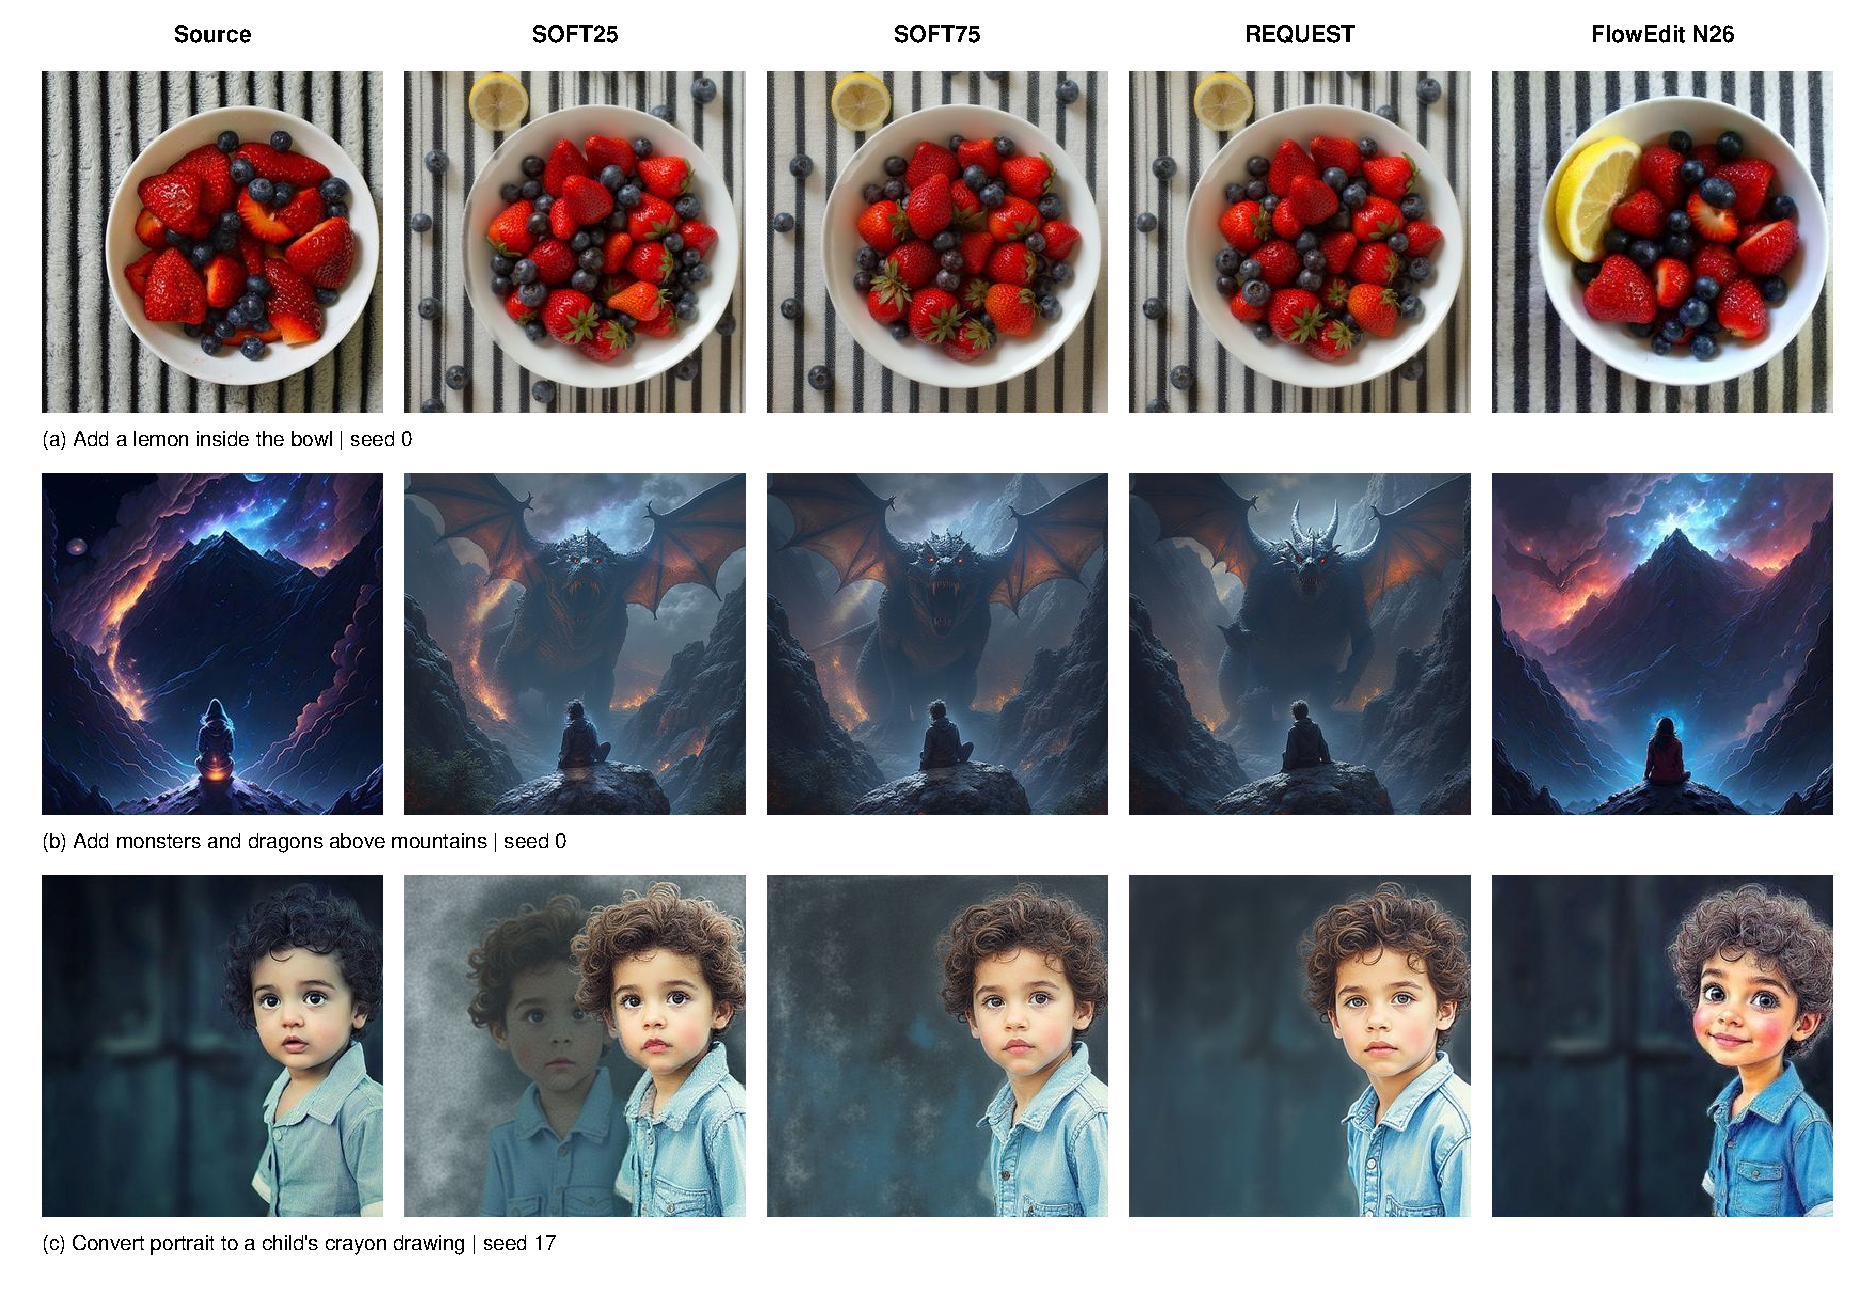
\includegraphics[width=.98\textwidth]{figures/r82_request_examples.pdf}
\caption{Selected completed support-study outputs. Rows show: adding a lemon inside the berry bowl (seed 0), adding monsters and dragons above mountains (seed 0), and converting a portrait to a child's crayon drawing (seed 17). REQUEST\_SOFT25 (memory-fixed) places the lemon beside the bowl; FlowEdit places it inside in this seed. The request/soft variants generate a visible dragon in the second row. In the third row REQUEST\_SOFT25 (memory-fixed) reduces the prominent duplicate-face structure visible in SOFT25, while the requested crayon appearance remains weak. Examples illustrate distinct outcomes, not aggregate success rates.}
\label{fig:r82-qualitative}
\end{figure*}

Across both seeds, the pepper-under-towel request leaves the pepper on top. Lemon addition often produces the requested object outside the bowl. Yellow-kitten outputs vary between partial cream coloration and stronger orange coloration with changed pose. Rough-sea edits often produce waves, with an extra foreground structure in one REQUEST\_SOFT25 (memory-fixed) output. Glass-to-wood and crystal-lamp requests produce changes in opacity or decoration with inconsistent target material. Olive removal often succeeds alongside changes to bowls, cloth, or surrounding objects. Wolf and dragon requests show visible semantic changes in some outputs. The portrait-style task retains rendered portrait appearance in many outputs, with varying duplicate-face artifacts. These findings motivate measuring requested relations and attributes alongside retention.

% Full twenty-sheet observations supplied by the parent review; the three
% illustrated source/seed sheets were also inspected during figure preparation.
\subsection{Request-Conditioned Memory}
\label{sec:r83-completed}
\subsubsection{Completed design and matched comparison population}
We compare seven memory and correction configurations on the same ten seen development sources, one per official category, with two seeds per source. REQUEST\_MEMORY, REQUEST\_BOTH, and MEAN\_MEMORY vary memory allocation; U25\_KV, FlowEdit N26, SOFT75, and REQUEST\_SOFT25 (memory-fixed) provide references matched on source, task, seed, and prompts.

Let $E$ be the native request-response map and $P=1-0.75E$ its protection weight. Three memory-off reference states each receive one source-prompt and one target-prompt evaluation, giving six native transformer probes. Average pooling over the same $2\times2$ latent patches used by FLUX packing maps $P$ from the $64\times64$ spatial grid to query weights $P_q$ on the $32\times32$ token grid. REQUEST\_MEMORY multiplies the inherited query-memory gate by $P_q$ while retaining global quarter-strength correction. REQUEST\_BOTH combines this spatial memory multiplier with request-routed ONLINE correction. MEAN\_MEMORY uses the same request-routed correction and replaces $P_q$ with its spatial mean. Source K/V pools, target-text contribution, attention blocks, and the first seven active memory steps remain fixed.

The mean control isolates spatial allocation from average memory attenuation. The recorded mean multiplier is identical between REQUEST\_BOTH and MEAN\_MEMORY in every paired slot, averaging 0.7359 across records. Their realized step-averaged gate values differ by at most 0.00046. This control matches the mean query multiplier; attention energy and the subsequent edited trajectories remain measured consequences of the allocation.

\subsubsection{Pixel measurements and source-level estimates}
Archived pixel measurements compare generated outputs with the source on a $512\times512$ grid. Whole-image NCC is source correlation. Its boundary-spanning crop permits only zero displacement, so fixed and shift-search NCC coincide. Global and edit-region MAE cover all ten sources. Preservation MAE uses eight sources and sixteen records per configuration: the lemon-addition source 223000000008 and crayon-style source 922000000003 have empty preservation complements. Those observations remain missing for this metric.

\begin{table*}[t]
\centering\footnotesize
\setlength{\tabcolsep}{4pt}
\caption{Completed memory study on the same ten seen development sources and two seeds. Every row contains twenty records. Preservation MAE uses eight eligible sources; the other pixel metrics use ten. Edit-region MAE measures source departure. Times describe recorded executions. REQUEST\_SOFT25 (memory-fixed) retains the original all-query memory.}
\label{tab:r83-means}
\begin{tabular}{lrrrrrr}
\toprule
Configuration & Global MAE & Whole NCC $\uparrow$ & Preservation MAE $\downarrow$ & Edit MAE & NFE & Time (s)\\
\midrule
REQUEST\_MEMORY & 0.1318 & 0.7444 & 0.1148 & 0.1491 & 97 & 55.63\\
REQUEST\_BOTH & 0.1296 & 0.7255 & 0.1093 & 0.1589 & 97 & 45.58\\
MEAN\_MEMORY & 0.1316 & 0.7221 & 0.1095 & 0.1581 & 97 & 45.80\\
U25\_KV & 0.1250 & 0.7635 & 0.1114 & 0.1380 & 91 & 43.38\\
FlowEdit N26 & 0.1271 & 0.7163 & 0.1032 & 0.1645 & 52 & 30.78\\
SOFT75 & 0.1273 & 0.7668 & 0.1147 & 0.1384 & 91 & 43.71\\
\shortstack[l]{REQUEST\_SOFT25\\(memory-fixed)} & 0.1227 & 0.7446 & 0.1060 & 0.1464 & 97 & 45.42\\
\bottomrule
\end{tabular}
\end{table*}

For each comparison, we first average paired differences over the two seeds within a source, then give each source equal weight. Percentile 95\% intervals use 20,000 bootstrap resamples of source means. Table~\ref{tab:r83-pairs} reports exploratory intervals without multiple-comparison adjustment.

\begin{table}[t]
\centering\scriptsize
\caption{Source-paired differences, first configuration minus reference. MAE uses normalized RGB values. NCC uses the whole image. Each cell gives mean difference and source-bootstrap 95\% interval. Preservation uses eight source clusters; other columns use ten. BOTH, MEAN, and MEMORY denote REQUEST\_BOTH, MEAN\_MEMORY, and REQUEST\_MEMORY; REQ denotes REQUEST\_SOFT25 (memory-fixed); MEM denotes REQUEST\_MEMORY.}
\label{tab:r83-pairs}
\setlength{\tabcolsep}{2pt}
\begin{tabular}{lrrr}
\toprule
Comparison & Whole NCC & Pres. MAE & Edit MAE\\
\midrule
BOTH $-$ MEAN & \shortstack{$0.0034$\\$[-0.0041,0.0127]$} & \shortstack{$-0.0003$\\$[-0.0020,0.0012]$} & \shortstack{$0.0008$\\$[-0.0051,0.0050]$}\\
MEM $-$ U25 & \shortstack{$-0.0191$\\$[-0.0321,-0.0077]$} & \shortstack{$0.0034$\\$[0.0003,0.0077]$} & \shortstack{$0.0112$\\$[0.0060,0.0170]$}\\
BOTH $-$ REQ & \shortstack{$-0.0191$\\$[-0.0298,-0.0095]$} & \shortstack{$0.0033$\\$[0.0001,0.0076]$} & \shortstack{$0.0125$\\$[0.0072,0.0183]$}\\
\bottomrule
\end{tabular}
\end{table}

\subsubsection{Spatial allocation and memory release}
REQUEST\_BOTH minus MEAN\_MEMORY gives a whole-image NCC difference of $0.0034$, with interval $[-0.0041,0.0127]$; six sources increase and four decrease. Preservation MAE differs by $-0.0003$, with interval $[-0.0020,0.0012]$, with three sources improving and five worsening. The estimates are small and uncertain: the intervals allow effects in either direction, and no equivalence margin was specified. They leave the value of spatial placement relative to mean attenuation open.

REQUEST\_MEMORY increases preservation MAE by 0.0034 relative to U25 and reduces NCC by 0.0191. Six of eight sources have greater preservation error, and nine of ten have lower NCC. With request-routed correction already present, REQUEST\_BOTH increases preservation MAE by 0.0033 and reduces NCC by 0.0191 relative to REQUEST\_SOFT25 (memory-fixed), with the same source-level directions. Edit-region departure increases on every source in both comparisons. These pixel results locate additional change inside and outside the official edit regions. Its value for the requested transformation depends on the task, as illustrated by the style improvement and relational failures below.

\noindent\textbf{Post hoc sensitivity of the memory comparison.}
For the archived ten-source spatial-minus-mean whole-image NCC difference, the mean is $0.0034$. Removing the crayon source, whose source-level difference is $0.0377$, gives $-0.0004$ across the remaining nine sources. This post hoc analysis shows sensitivity to source composition; the primary estimate retains all ten sources.

\subsubsection{Visible style gains and persistent relational errors}
The qualitative review covered all twenty paired comparison sheets across both seeds. Figure~\ref{fig:r83-memory-examples} displays three source--seed cases with the original delivered previews and a common column order. In the crayon-style case at seed 17, all three new configurations move toward a hand-drawn cartoon appearance. REQUEST\_BOTH shows a particularly clear drawn rendering of the face, hair, and shirt compared with REQUEST\_SOFT25 (memory-fixed). This is a positive, task-specific signal from memory release. MEAN\_MEMORY also strengthens the illustrated appearance but contains a conspicuous secondary face in the background. Spatial and mean memory attenuation can thus reach similar aggregate source correlations while differing in a visible artifact.

\begin{figure*}[t]
\centering
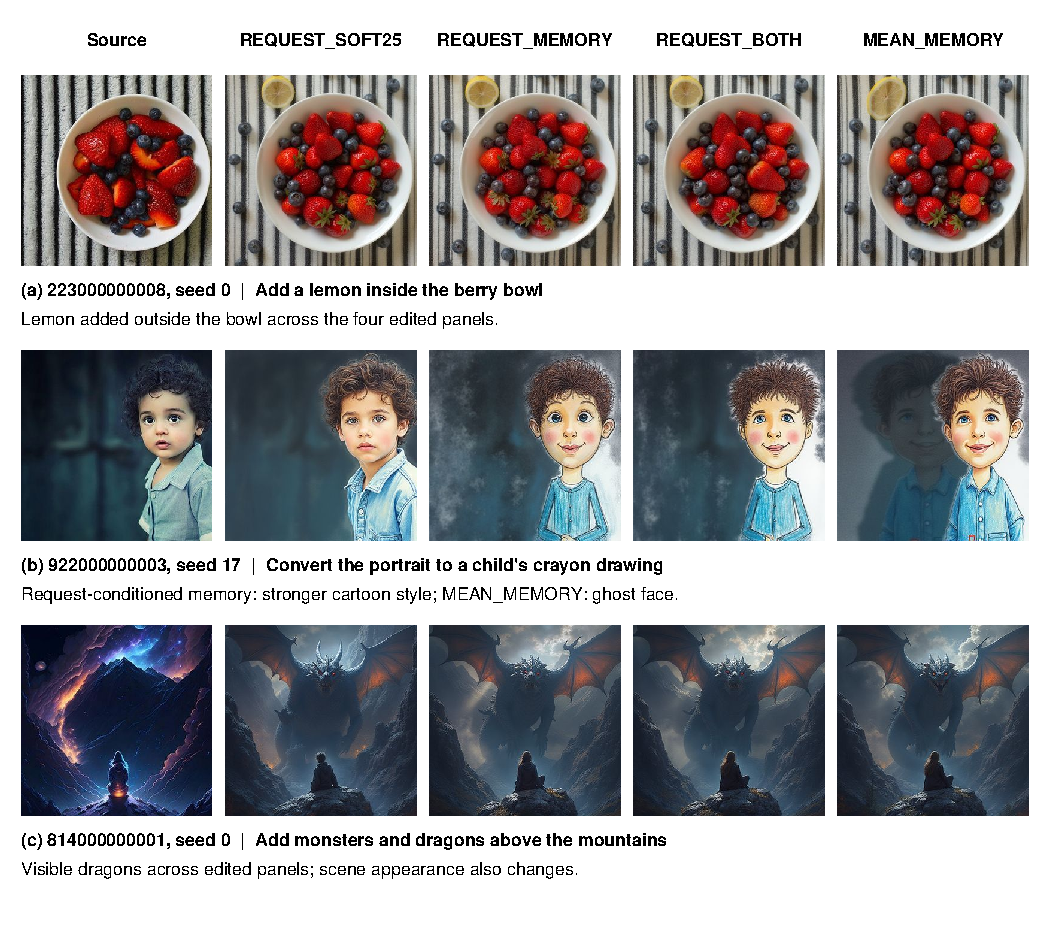
\includegraphics[width=.99\textwidth,height=.72\textheight,keepaspectratio]{figures/r83_memory_examples.pdf}
\caption{Completed request-memory examples. Columns: source, frozen REQUEST\_SOFT25 (memory-fixed), REQUEST\_MEMORY, REQUEST\_BOTH, and MEAN\_MEMORY. Top: source 223000000008, seed 0; the added lemon remains outside the berry bowl in all four edited panels. Middle: source 922000000003, seed 17; the three new configurations show stronger hand-drawn cartoon appearance, especially REQUEST\_BOTH, while MEAN\_MEMORY contains a ghost face. Bottom: source 814000000001, seed 0; every edited panel contains a visible dragon, with changes to the scene. Rows illustrate distinct requested outcomes and artifacts; labels occupy separate strips outside the image panels.}
\label{fig:r83-memory-examples}
\end{figure*}

Object presence and spatial relations remain distinct outcomes. In the lemon case at seed 0, all four displayed edited configurations add a lemon beside the bowl, leaving the requested inside relation unmet. The full review also finds the pepper still above the towel at seed 17 and transparent vessels remaining in the wooden-cup request at seed 0. The dragon example shows a visible requested addition across configurations, together with scene changes. These observations connect the increased edit-region departure to both useful stylistic change and persistent relational or material errors.

\subsubsection{Realized budgets and cost}
Each new configuration costs 97 standalone NFE: 28 inversion evaluations, 28 current-source evaluations, 28 target-generation evaluations, seven source-reference memory captures, and six native response probes. The probe count is identical for the mean control. Compared with U25's 91 NFE, the increase is six calls, or 6.6\%; REQUEST\_SOFT25 (memory-fixed) already uses 97 NFE.

Mean cumulative correction impulses are 0.2370 for REQUEST\_MEMORY, 0.2367 for REQUEST\_BOTH, and 0.2376 for MEAN\_MEMORY, versus 0.2319 for U25 and 0.2306 for REQUEST\_SOFT25 (memory-fixed). The ONLINE coefficient remains 0.25, with normalization errors below $1.6\times10^{-8}$ in the two new routed arms. The actual cumulative impulse varies with the edited trajectory. REQUEST\_BOTH and MEAN\_MEMORY average 45.58 and 45.80 seconds; run-level variability is documented in the provenance appendix.

\subsection{Development dose response and controls}
\label{sec:development-dose}
The development study completes 130 of 130 outputs with successful automatic evaluation on ten previously used sources, one per official category. Six configurations use seeds 0 and 17; deterministic RF-Edit I08 uses seed 0 once per source. Table~\ref{tab:development-dose} reports all seven configurations. Means first average seeds within source and then weight sources equally. CLIP and full-image DINO and LPIPS use ten sources; preservation MAE and LPIPS use eight, excluding two empty official preservation complements. Evaluation masks are independent of the request-conditioned routing support. This population is kept separate from the 40-source independent evaluation.

\paragraph{From normalized routing to direct local correction.}
Historical ONLINE correction restores the global quarter-strength RMS after routing, applying $0.25\RMS(c_i)P\odot c_i/\RMS(P\odot c_i)$. Direct local correction applies $\lambda P\odot c_i$ with $P=1-0.75E$ and no restoration. This transition preserves the request-conditioned spatial support and the first-seven-step source-memory window while allowing support to attenuate the instantaneous correction. The coefficient sweep $\lambda\in\{0.15,0.25,0.35\}$ studies the resulting strength dependence. CORR25 remains the fixed primary configuration, and BOTH25 adds the secondary spatial query-memory gate.

ENERGY calibrates the global direction at its own current state to the RMS that $0.25P\odot c_i$ would have at that same state. It supplies a counterfactual same-state magnitude control; the independently evolving arms retain their own residuals and cumulative correction energies. CORR, BOTH, and ENERGY each use three native prompt-response probes (six extra calls) and cost 97 standalone NFE.

\begin{table*}[t]
\centering\small
\caption{Ten-source development study: all seven configurations and 130 outputs. CLIP and DINO are higher-is-better; LPIPS and preservation MAE are lower-is-better. Full-image metrics use ten sources and preservation metrics use eight. Each non-RF-Edit arm has 20 outputs; RF-Edit has ten. NFE counts all standalone transformer evaluations.}
\label{tab:development-dose}
\label{tab:r84-dose}
\setlength{\tabcolsep}{4pt}
\begin{tabular}{lrrrrrrr}
\toprule
Configuration & CLIP target $\uparrow$ & CLIP dir. $\uparrow$ & DINO $\uparrow$ & LPIPS full $\downarrow$ & LPIPS preserved $\downarrow$ & Pres. MAE $\downarrow$ & NFE\\
\midrule
Local correction 0.15 & 0.2618 & 0.0964 & 0.5543 & 0.5827 & 0.5544 & 0.1600 & 97\\
TraceMemory (CORR25) & 0.2609 & 0.0979 & 0.5946 & 0.5276 & 0.4983 & 0.1284 & 97\\
Local correction 0.35 & 0.2562 & 0.0939 & 0.6063 & 0.4803 & 0.4561 & 0.1055 & 97\\
BOTH25 (secondary) & 0.2659 & 0.1145 & 0.5202 & 0.5444 & 0.5145 & 0.1338 & 97\\
ENERGY\_MATCH25 & 0.2599 & 0.0957 & 0.5967 & 0.5396 & 0.5115 & 0.1341 & 97\\
FlowEdit N28 & 0.2809 & 0.1549 & 0.4728 & 0.6144 & 0.5293 & 0.2014 & 56\\
RF-Edit I08 & 0.2511 & 0.0451 & 0.8071 & 0.2766 & 0.2548 & 0.0452 & 100\\
\bottomrule
\end{tabular}
\end{table*}

Within these ten development sources, increasing the local coefficient from 0.15 through 0.25 to 0.35 gives monotonic decreases in preservation MAE (0.1600, 0.1284, 0.1055), full-image LPIPS (0.5827, 0.5276, 0.4803), and preservation LPIPS (0.5544, 0.4983, 0.4561), together with increasing mean DINO (0.5543, 0.5946, 0.6063). These are aggregate dose trends within a matched population. Relative to 0.15, CORR25 changes full-image and preservation LPIPS by $-0.0551$ and $-0.0561$; relative to 0.35, the differences are $+0.0473$ and $+0.0422$. All four LPIPS contrasts have within-metric Holm $p\leq0.0469$. Target and directional CLIP difference intervals span zero in both dose comparisons. The sweep demonstrates a correction-strength dependence of source retention; spatial allocation is examined separately through the same-state ENERGY control. Dose means from these seen sources and benchmark means from the independent population describe their respective matched comparisons.


\section{Final Evaluated Local Correction and Memory Study}
\label{sec:final-evaluation}
\subsection{Completed population, method, and evaluation}
The independent R85 study completes 520 of 520 outputs with successful automatic evaluation on 40 sources, four per official category. Six arms use seeds 0 and 17; deterministic RF-Edit I08 uses seed 0 once per source. The source is the statistical unit: we average seeds within each source and give sources equal weight. The primary method is TraceMemory (CORR25); BOTH25 is the preregistered secondary spatial-memory configuration. R84 provides the separate seen-source dose study: all 130 outputs from ten sources completed automatic evaluation. Development and independent populations are not pooled.

The method uses only source and target prompts to construct $E$ and $P=1-0.75E$. Official edit annotations enter evaluation only. The primary correction is $0.25P\odot c_i$ without RMS restoration. Its first-seven-step full-source, all-query memory is unchanged. BOTH additionally pools $P$ to the packed image-query grid. ENERGY uses Eq.~\eqref{eq:energy-control}, preserving the global residual direction at the local rule's same-state RMS. These three arms each cost 97 standalone NFE, including six native probe calls.

Target and directional CLIP use ViT-L/14; DINO uses full-image DINOv2-base cosine similarity. AlexNet LPIPS is reported for the whole image and as a spatial-map average weighted by the area-resampled official preservation complement. LPIPS feature receptive fields can cross that boundary. All 40 sources contribute full-image metrics; preservation metrics use 33 sources, with seven empty complements omitted. R84 analogously uses ten full-image and eight preservation-eligible sources. Full-image source distance includes requested changes, so preservation LPIPS is the regional retention comparison.

\begin{table*}[t]
\centering\small
\caption{Final R85 evaluation: equal-source means on 40 independent sources and seven methods. CLIP target, directional CLIP, and full-image DINO are higher-is-better; LPIPS is lower-is-better. Preservation LPIPS uses 33 sources. Six arms have 80 outputs each; RF-Edit has 40. NFE is the complete standalone transformer-call count.}
\label{tab:final-means}
\setlength{\tabcolsep}{5pt}
\begin{tabular}{lrrrrrr}
\toprule
Method & CLIP target $\uparrow$ & CLIP dir. $\uparrow$ & DINO $\uparrow$ & LPIPS full $\downarrow$ & LPIPS preserved $\downarrow$ & NFE\\
\midrule
TraceMemory (CORR25) & 0.2629 & 0.0863 & 0.5904 & 0.5419 & 0.5142 & 97\\
BOTH25 (secondary) & 0.2733 & 0.1069 & 0.5579 & 0.5620 & 0.5269 & 97\\
ENERGY\_MATCH25 & 0.2622 & 0.0881 & 0.5856 & 0.5483 & 0.5226 & 97\\
U25\_KV & 0.2632 & 0.0908 & 0.6111 & 0.4971 & 0.4743 & 91\\
FlowEdit N26 & 0.2712 & 0.1177 & 0.5737 & 0.4437 & 0.4281 & 52\\
RF-Inversion ETA03 & 0.2694 & 0.1065 & 0.4670 & 0.5431 & 0.5322 & 56\\
RF-Edit I08 & 0.2453 & 0.0383 & 0.7875 & 0.2778 & 0.2688 & 100\\
\bottomrule
\end{tabular}
\end{table*}

\subsection{Source-paired estimates and localization benefit}
Pointwise percentile 95\% intervals use 10,000 source-bootstrap resamples. Two-sided source sign-flip tests use 10,000 Monte Carlo draws with plus-one correction. The planned Holm family contains six CORR25 comparisons separately within each metric, including BOTH and RF-Edit; Table~\ref{tab:final-paired} reports this adjusted $p$. RF-Edit's single deterministic result is compared with each other arm's two-seed source mean.

CORR25 reduces preservation LPIPS relative to ENERGY by 0.0084, with interval $[-0.0143,-0.0022]$ and adjusted $p=0.0238$. Full-image LPIPS decreases by 0.0064 ($p=0.0014$). This is a modest measured benefit from request-conditioned allocation beyond the global same-state magnitude control. Target CLIP differs by $+0.0007$ and directional CLIP by $-0.0018$, with intervals spanning zero; the target and directional CLIP intervals both span zero. Each arm evolves on its own trajectory, with its own cumulative correction energy.

\begin{table*}[t]
\centering\footnotesize
\caption{Selected final source-paired effects. Differences are first arm minus second. Intervals are pointwise 95\% source-bootstrap intervals; $p_{\rm H}$ uses six planned comparisons per metric. BOTH--CORR25 is the sign-reversed member of that family. Source counts are 33 for preservation LPIPS and 40 otherwise.}
\label{tab:final-paired}
\setlength{\tabcolsep}{5pt}
\begin{tabular}{llrrr}
\toprule
Comparison & Metric & Difference & 95\% interval & $p_{\rm H}$\\
\midrule
CORR25 $-$ ENERGY & LPIPS preserved & $-0.0084$ & $[-0.0143,-0.0022]$ & 0.0238\\
CORR25 $-$ ENERGY & LPIPS full & $-0.0064$ & $[-0.0098,-0.0030]$ & 0.0014\\
CORR25 $-$ ENERGY & Directional CLIP & $-0.0018$ & $[-0.0066,0.0030]$ & 0.5297\\
CORR25 $-$ FlowEdit & Directional CLIP & $-0.0315$ & $[-0.0504,-0.0137]$ & 0.0084\\
CORR25 $-$ FlowEdit & LPIPS preserved & $+0.0861$ & $[0.0500,0.1224]$ & 0.0006\\
CORR25 $-$ FlowEdit & DINO & $+0.0167$ & $[-0.0326,0.0704]$ & 1.0000\\
CORR25 $-$ U25 & LPIPS preserved & $+0.0399$ & $[0.0331,0.0469]$ & 0.0006\\
BOTH $-$ CORR25 & Target CLIP & $+0.0104$ & $[0.0054,0.0159]$ & 0.0006\\
BOTH $-$ CORR25 & Directional CLIP & $+0.0207$ & $[0.0099,0.0334]$ & 0.0012\\
BOTH $-$ CORR25 & LPIPS preserved & $+0.0127$ & $[0.0077,0.0180]$ & 0.0006\\
BOTH $-$ CORR25 & DINO & $-0.0325$ & $[-0.0591,-0.0109]$ & 0.0160\\
CORR25 $-$ ETA03 & DINO & $+0.1234$ & $[0.0700,0.1826]$ & 0.0010\\
\bottomrule
\end{tabular}
\end{table*}

\subsection{Benchmark position and memory trade-off}
FlowEdit N26 has higher directional CLIP and lower full-image and preservation LPIPS than CORR25, using 52 rather than 97 NFE. CORR25 minus FlowEdit gives directional CLIP $-0.0315$ ($p_{\rm H}=0.0084$) and preservation LPIPS $+0.0861$ ($p_{\rm H}=0.0006$). The DINO difference is $+0.0167$ with interval $[-0.0326,0.0704]$, leaving its direction uncertain. U25 has lower full-image and preservation LPIPS, higher mean DINO, and slightly higher CLIP means at 91 NFE. FlowEdit combines stronger directional CLIP with lower LPIPS and fewer evaluations; U25 also has lower LPIPS at fewer evaluations. CORR25 improves full-image DINO over RF-Inversion ETA03 by 0.1234 ($p_{\rm H}=0.0010$), while RF-Edit emphasizes retention with lower semantic alignment.

BOTH increases both semantic proxies: target CLIP increases by 0.0104 and directional CLIP by 0.0207 relative to CORR25. Preservation LPIPS increases by 0.0127, full-image LPIPS by 0.0201, and DINO decreases by 0.032496. Spatial memory attenuation therefore releases more prompt-driven change together with more source departure. The primary and secondary roles were fixed before the independent evaluation.

\begin{figure*}[t]
\centering
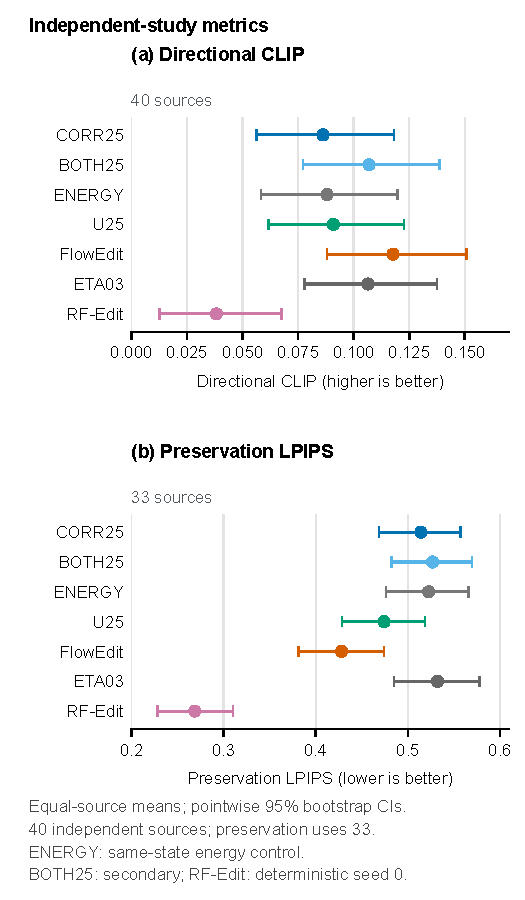
\includegraphics[width=.96\textwidth]{figures/final_metrics.pdf}
\caption{Final R85 metrics in a common arm order. The two horizontal-dot panels show source-level mean directional CLIP and preservation LPIPS with pointwise 95\% source-bootstrap intervals. Directional CLIP uses 40 sources; preservation LPIPS uses 33. Intervals describe each mean, while Table~\ref{tab:final-paired} reports paired differences.}
\label{fig:final-metrics}
\end{figure*}

\subsection{Development dose response and qualitative cases}
R84 evaluates the frozen direct local coefficients 0.15, 0.25, and 0.35 on ten seen sources (Table~\ref{tab:r84-dose}). Increasing correction strength lowers both full-image and preservation LPIPS. Relative to 0.15, CORR25 changes these metrics by $-0.0551$ and $-0.0561$; relative to 0.35, the differences are $+0.0473$ and $+0.0422$. All four comparisons have within-metric Holm $p\leq0.046875$. Target and directional CLIP difference intervals span zero in both dose comparisons. This development result identifies a preservation response to correction strength; the primary coefficient and BOTH's secondary role remain fixed for R85.

\begin{table*}[t]
\centering\small
\caption{R84 seen-source dose study. Means use ten sources for CLIP and DINO, eight for preservation LPIPS, and two seeds per source. Each arm costs 97 NFE. The complete R84 evaluation has 130 outputs including its other controls.}
\label{tab:r84-dose}
\begin{tabular}{lrrrrrr}
\toprule
Local coefficient & CLIP target & CLIP dir. & DINO & LPIPS full & LPIPS preserved & NFE\\
\midrule
0.15 & 0.2618 & 0.0964 & 0.5543 & 0.5827 & 0.5544 & 97\\
0.25 & 0.2609 & 0.0979 & 0.5946 & 0.5276 & 0.4983 & 97\\
0.35 & 0.2562 & 0.0939 & 0.6063 & 0.4803 & 0.4561 & 97\\
\bottomrule
\end{tabular}
\end{table*}

\begin{figure*}[t]
\centering
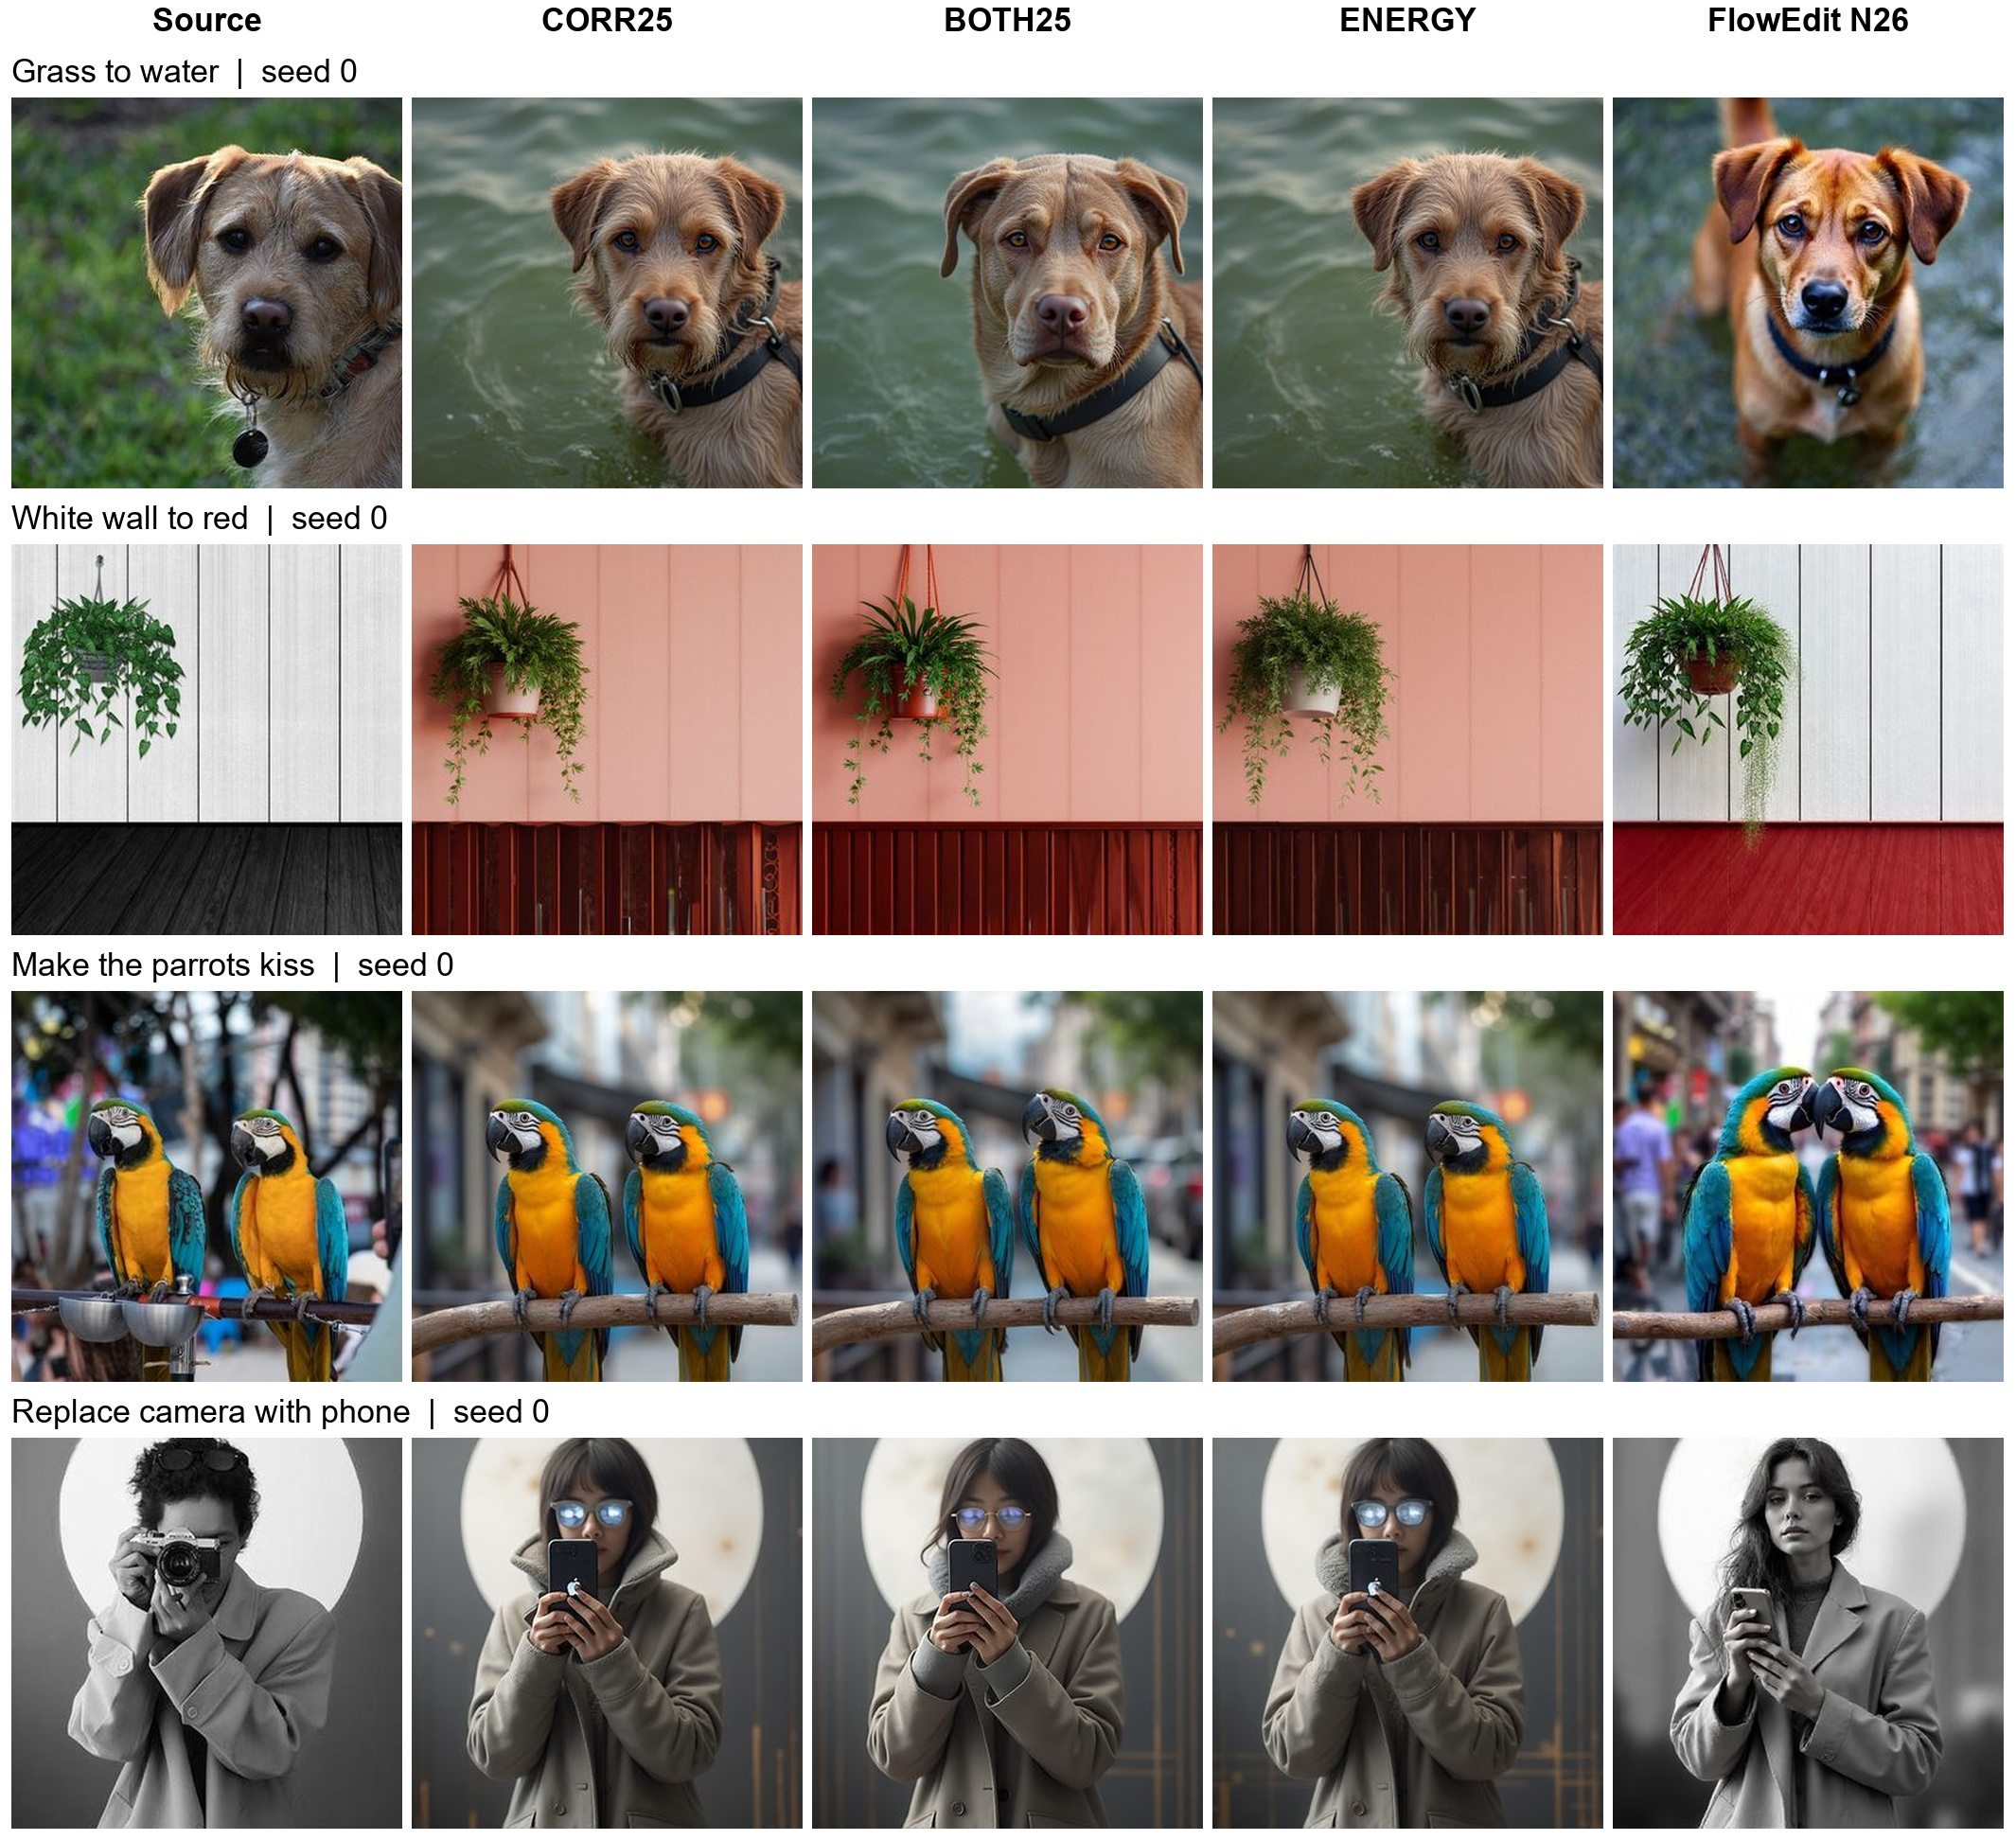
\includegraphics[width=.98\textwidth]{figures/final_qualitative.jpg}
\caption{Final seed-0 qualitative comparisons. Columns: source, TraceMemory (CORR25), ENERGY\_MATCH25, and FlowEdit. Rows show grass-to-water, wall-to-red, parrots-kissing, and camera-to-phone requests. The common examples expose appearance changes and requested relational or category changes alongside source retention; quantitative conclusions use the full source population.}
\label{fig:final-qualitative}
\end{figure*}


\section{Qualitative Findings and Limitations}
\label{sec:limitations}
\textbf{Patterns and identity.} Source-like musical notes and shirt graphics improve in the regional examples, while cup handles, faces, and exact glyph arrangements can still change. The rug retains a grid-like texture in some outputs while individual cells and borders are rewritten. These cases motivate distinct subject-identity and exact-pattern judgments rather than a single source-similarity score.

\textbf{Requested attributes.} Cup and floor examples show visible lighting and material changes. The dog/snow example retains substantial grass despite falling snow. Rain streaks do not establish wet fur or a wet paved contact surface. Butterfly warmth alone does not establish the requested left-side low-angle light and directional shadows. Figure~\ref{fig:failures} gathers specific failures; all tasks and seeds remain available in the complete gallery.

\begin{figure*}[t]
\centering
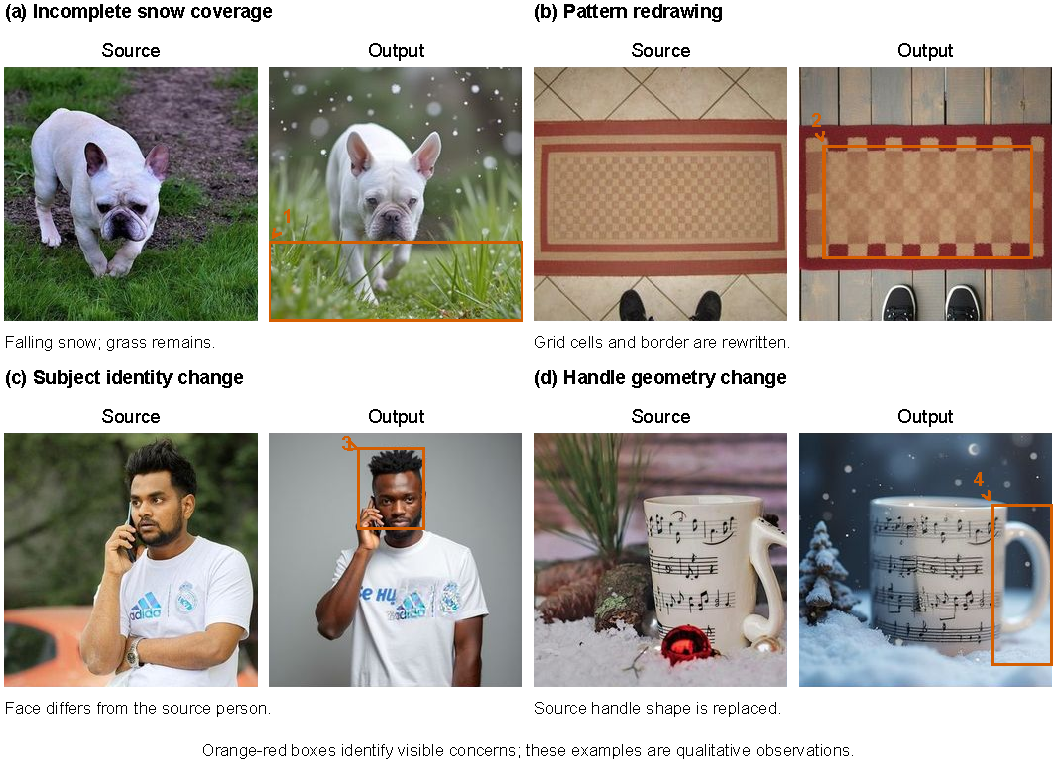
\includegraphics[width=.98\textwidth,height=.72\textheight,keepaspectratio]{figures/failure_cases.pdf}
\caption{Four failure categories, each presented as a source/output pair with orange-red localization boxes. Panels (a)--(d): dog/snow seed 17 with unfiltered external-profile ROI correction; rug/floor seed 17 with ONLINE/all; printed shirt seed 17 with ONLINE/ROI-query memory; cup/night seed 10 with ONLINE/all. Visible concerns are incomplete snow coverage, rewritten grid details, changed identity, and changed object geometry. These examples motivate separate edit, subject, pattern, and artifact labels.}
\label{fig:failures}
\end{figure*}

\textbf{Annotation and population.} The supplied-region studies evaluate targeted protection using a manual region for both routing and local scoring. The 24-source contrast-routing pilot adds 24 sources that were new at selection, automatic source-contrast masks, and official evaluation regions kept separate from the method. It exposes increased preservation-region error for the automatic variant. Contrast selects edges and textures irrespective of the requested change; object and edit semantics require additional information or a less selective allocation. These pilot sources subsequently informed development. The final independent evaluation uses 40 separately selected sources and is reported in Section~\ref{sec:final-evaluation}.

\textbf{Magnitude and cost.} Historical ONLINE restoration concentrates a global RMS target through regional support. Direct local correction removes this amplification, and its retention depends on the chosen coefficient. The support estimator adds six transformer calls to the 91-call memory-enabled editor. The final comparison evaluates one frozen primary coefficient and one frozen memory variant; the three-point dose study characterizes the development population. Regional LPIPS and full-image DINO capture different aspects of preservation, as the spatial and identity changes in Fig.~\ref{fig:final-qualitative} illustrate.

\textbf{Outcome coverage.} The reported benchmark measures text alignment through CLIP, broad source similarity through DINO, and regional perceptual distance through LPIPS. Exact relations, instance identity, and visible artifacts require task-specific judgments. Appendix~\ref{sec:review-protocol} defines a method-anonymized local vision-language evaluation for these outcomes, with a common task rubric and source-level aggregation.

\section{Conclusion}
TraceMemory separates the location and magnitude of source correction from the coverage of source attention. The support-energy relation explains how global RMS restoration amplifies a regional update. The frozen direct-local configuration improves preservation-region LPIPS by 0.0084 relative to a global control calibrated to the same-state correction energy. Increasing the local coefficient improves retention across the three development doses, while request-conditioned memory gating strengthens text alignment and increases perceptual source departure. Together, these results identify a controlled localization benefit and quantify the distinct roles of correction dose and memory release. Task-level identity, exact relations, and artifact judgments remain the next outcome layer for evaluating the operating points represented by these automatic scores.

\FloatBarrier
\begin{thebibliography}{46}
\raggedright
% Insert within the parent thebibliography; existing keys intentionally preserved.
\bibitem{rout2025rfinversion} Litu Rout, Yujia Chen, Nataniel Ruiz, Constantine Caramanis, Sanjay Shakkottai, and Wen-Sheng Chu, \textit{Semantic Image Inversion and Editing using Rectified Stochastic Differential Equations}, International Conference on Learning Representations, 2025. \url{https://arxiv.org/abs/2410.10792}.
\bibitem{wang2025rfsolver} Jiangshan Wang, Junfu Pu, Zhongang Qi, Jiayi Guo, Yue Ma, Nisha Huang, Yuxin Chen, Xiu Li, and Ying Shan, \textit{Taming Rectified Flow for Inversion and Editing}, Proceedings of the 42nd International Conference on Machine Learning, vol. 267, pp. 64044--64058, 2025. \url{https://proceedings.mlr.press/v267/wang25ce.html}.
\bibitem{kim2025reflex} Jimyeong Kim, Jungwon Park, Yeji Song, Nojun Kwak, and Wonjong Rhee, \textit{{ReFlex}: Text-Guided Editing of Real Images in Rectified Flow via Mid-Step Feature Extraction and Attention Adaptation}, Proceedings of the IEEE/CVF International Conference on Computer Vision, pp. 15939--15948, 2025. \url{https://arxiv.org/abs/2507.01496}.
\bibitem{kulikov2025flowedit} Vladimir Kulikov, Matan Kleiner, Inbar Huberman-Spiegelglas, and Tomer Michaeli, \textit{{FlowEdit}: Inversion-Free Text-Based Editing Using Pre-Trained Flow Models}, Proceedings of the IEEE/CVF International Conference on Computer Vision, pp. 19721--19730, 2025. \url{https://openaccess.thecvf.com/content/ICCV2025/html/Kulikov_FlowEdit_Inversion-Free_Text-Based_Editing_Using_Pre-Trained_Flow_Models_ICCV_2025_paper.html}.
\bibitem{yang2026directedit} Desong Yang and Mang Ye, \textit{{DirectEdit}: Step-Level Accurate Inversion for Flow-Based Image Editing}, Proceedings of the 43rd International Conference on Machine Learning, vol. 306, pp. 146750--146765, 2026. \url{https://proceedings.mlr.press/v306/yang26cy.html}.
\bibitem{tang2026wavelet} Anqi Tang, Wenhao Sun, and Zhaoqiang Liu, \textit{Wavelet-Guided Semantic Signal Compensation for Inversion-Free Image Editing}, Computer Vision -- ECCV 2026, vol. 17019, pp. 671--688, 2026. \url{https://link.springer.com/chapter/10.1007/978-3-032-37550-6_38}. Method equations cited from \url{https://arxiv.org/abs/2607.02421v1}.
\bibitem{li2025cvc} Zixiang Li, Yue Song, Jianing Peng, Ting Liu, Jun Huang, Xiaochao Qu, Luoqi Liu, Wei Wang, Yao Zhao, and Yunchao Wei, \textit{On Exact Editing of Flow-Based Diffusion Models}, arXiv:2512.24015 (2025; revised 2026). \url{https://arxiv.org/abs/2512.24015}. Method equations cited from version 2.
\bibitem{kim2025flowalign} Jeongsol Kim, Yeobin Hong, Jonghyun Park, and Jong Chul Ye, \textit{FlowAlign: Trajectory-Regularized, Inversion-Free Flow-based Image Editing}, arXiv:2505.23145 (2025). \url{https://arxiv.org/abs/2505.23145}.
\bibitem{liao2025freqedit} Yucheng Liao, Jiajun Liang, Kaiqian Cui, Baoquan Zhao, Haoran Xie, Wei Liu, Qing Li, and Xudong Mao, \textit{FreqEdit: Preserving High-Frequency Features for Robust Multi-Turn Image Editing}, arXiv:2512.01755, 2025 (revised 2026). \url{https://arxiv.org/abs/2512.01755}. Method comparison uses v1, Secs.~4.2--4.4.
\bibitem{deng2025fireflow} Yingying Deng, Xiangyu He, Changwang Mei, Peisong Wang, and Fan Tang, \textit{FireFlow: Fast Inversion of Rectified Flow for Image Semantic Editing}, ICML, PMLR 267, pp. 13110--13128, 2025. \url{https://proceedings.mlr.press/v267/deng25c.html}.
\bibitem{avrahami2025stableflow} Omri Avrahami, Or Patashnik, Ohad Fried, Egor Nemchinov, Kfir Aberman, Dani Lischinski, and Daniel Cohen-Or, \textit{Stable Flow: Vital Layers for Training-Free Image Editing}, CVPR, 2025. \url{https://arxiv.org/abs/2411.14430}.
\bibitem{dalva2025fluxspace} Yusuf Dalva, Kavana Venkatesh, and Pinar Yanardag, \textit{FluxSpace: Disentangled Semantic Editing in Rectified Flow Models}, CVPR, 2025. \url{https://openaccess.thecvf.com/content/CVPR2025/papers/Dalva_FluxSpace_Disentangled_Semantic_Editing_in_Rectified_Flow_Models_CVPR_2025_paper.pdf}.
\bibitem{dao2026steerflow} Thinh Dao, Zhen Wang, Kien T. Pham, and Long Chen, \textit{SteerFlow: Steering Rectified Flows for Faithful Inversion-Based Image Editing}, arXiv:2604.01715, 2026. \url{https://arxiv.org/abs/2604.01715}.
\bibitem{zhou2025multiturn} Zijun Zhou, Yingying Deng, Xiangyu He, Weiming Dong, and Fan Tang, \textit{Multi-turn Consistent Image Editing}, ICCV, pp. 15792--15801, 2025. \url{https://openaccess.thecvf.com/content/ICCV2025/papers/Zhou_Multi-turn_Consistent_Image_Editing_ICCV_2025_paper.pdf}.
\bibitem{lupascu2026otrf} Marian Lupa\c{s}cu and Mihai Sorin Stupariu, \textit{Optimal Transport for Rectified Flow Image Editing: Unifying Inversion-Based and Direct Methods}, WACV, pp. 6764--6774, 2026. \url{https://openaccess.thecvf.com/content/WACV2026/papers/Lupascu_Optimal_Transport_for_Rectified_Flow_Image_Editing_Unifying_Inversion-Based_and_WACV_2026_paper.pdf}.

% Independent diffusion-editing literature slice, verified 2026-10-30.
% Exactly 15 distinct papers. Bibliography fragment: insert inside the existing
% thebibliography environment, reconciling existing keys rather than duplicating.
% ju2024pnpinversion also covers the Direct Inversion preprint (arXiv:2310.01506).
% This is distinct from tumanyan2023pnpfeatures.

\bibitem{ju2024pnpinversion}
Xuan Ju, Ailing Zeng, Yuxuan Bian, Shaoteng Liu, and Qiang Xu,
\textit{PnP Inversion: Boosting Diffusion-based Editing with 3 Lines of Code},
International Conference on Learning Representations (ICLR), 2024.
\url{https://proceedings.iclr.cc/paper_files/paper/2024/hash/661caac7729aa7d8c6b8ac0d39ccbc6a-Abstract-Conference.html}.

\bibitem{cao2023masactrl}
Mingdeng Cao, Xintao Wang, Zhongang Qi, Ying Shan, Xiaohu Qie, and Yinqiang Zheng,
\textit{MasaCtrl: Tuning-Free Mutual Self-Attention Control for Consistent Image Synthesis and Editing},
Proceedings of the IEEE/CVF International Conference on Computer Vision (ICCV), pp.~22560--22570, 2023.
\url{https://openaccess.thecvf.com/content/ICCV2023/html/Cao_MasaCtrl_Tuning-Free_Mutual_Self-Attention_Control_for_Consistent_Image_Synthesis_and_ICCV_2023_paper.html}.

\bibitem{hertz2023prompttoprompt}
Amir Hertz, Ron Mokady, Jay Tenenbaum, Kfir Aberman, Yael Pritch, and Daniel Cohen-Or,
\textit{Prompt-to-Prompt Image Editing with Cross-Attention Control},
International Conference on Learning Representations (ICLR), 2023.
\url{https://openreview.net/forum?id=_CDixzkzeyb}.

\bibitem{tumanyan2023pnpfeatures}
Narek Tumanyan, Michal Geyer, Shai Bagon, and Tali Dekel,
\textit{Plug-and-Play Diffusion Features for Text-Driven Image-to-Image Translation},
Proceedings of the IEEE/CVF Conference on Computer Vision and Pattern Recognition (CVPR), pp.~1921--1930, 2023.
\url{https://openaccess.thecvf.com/content/CVPR2023/html/Tumanyan_Plug-and-Play_Diffusion_Features_for_Text-Driven_Image-to-Image_Translation_CVPR_2023_paper.html}.

\bibitem{mokady2023nulltext}
Ron Mokady, Amir Hertz, Kfir Aberman, Yael Pritch, and Daniel Cohen-Or,
\textit{NULL-Text Inversion for Editing Real Images Using Guided Diffusion Models},
Proceedings of the IEEE/CVF Conference on Computer Vision and Pattern Recognition (CVPR), pp.~6038--6047, 2023.
\url{https://openaccess.thecvf.com/content/CVPR2023/html/Mokady_NULL-Text_Inversion_for_Editing_Real_Images_Using_Guided_Diffusion_Models_CVPR_2023_paper.html}.

\bibitem{wallace2023edict}
Bram Wallace, Akash Gokul, and Nikhil Naik,
\textit{EDICT: Exact Diffusion Inversion via Coupled Transformations},
Proceedings of the IEEE/CVF Conference on Computer Vision and Pattern Recognition (CVPR), pp.~22532--22541, 2023.
\url{https://openaccess.thecvf.com/content/CVPR2023/html/Wallace_EDICT_Exact_Diffusion_Inversion_via_Coupled_Transformations_CVPR_2023_paper.html}.

\bibitem{meng2022sdedit}
Chenlin Meng, Yutong He, Yang Song, Jiaming Song, Jiajun Wu, Jun-Yan Zhu, and Stefano Ermon,
\textit{SDEdit: Guided Image Synthesis and Editing with Stochastic Differential Equations},
International Conference on Learning Representations (ICLR), 2022.
\url{https://openreview.net/forum?id=aBsCjcPu_tE}.

\bibitem{avrahami2022blended}
Omri Avrahami, Dani Lischinski, and Ohad Fried,
\textit{Blended Diffusion for Text-Driven Editing of Natural Images},
Proceedings of the IEEE/CVF Conference on Computer Vision and Pattern Recognition (CVPR), pp.~18208--18218, 2022.
\url{https://openaccess.thecvf.com/content/CVPR2022/html/Avrahami_Blended_Diffusion_for_Text-Driven_Editing_of_Natural_Images_CVPR_2022_paper.html}.

\bibitem{avrahami2023blendedlatent}
Omri Avrahami, Ohad Fried, and Dani Lischinski,
\textit{Blended Latent Diffusion},
ACM Transactions on Graphics, vol.~42, no.~4, article~149, pp.~1--11, 2023.
\url{https://doi.org/10.1145/3592450}.

\bibitem{couairon2023diffedit}
Guillaume Couairon, Jakob Verbeek, Holger Schwenk, and Matthieu Cord,
\textit{DiffEdit: Diffusion-based semantic image editing with mask guidance},
International Conference on Learning Representations (ICLR), 2023.
\url{https://openreview.net/forum?id=3lge0p5o-M-}.

\bibitem{brooks2023instructpix2pix}
Tim Brooks, Aleksander Holynski, and Alexei A. Efros,
\textit{InstructPix2Pix: Learning To Follow Image Editing Instructions},
Proceedings of the IEEE/CVF Conference on Computer Vision and Pattern Recognition (CVPR), pp.~18392--18402, 2023.
\url{https://openaccess.thecvf.com/content/CVPR2023/html/Brooks_InstructPix2Pix_Learning_To_Follow_Image_Editing_Instructions_CVPR_2023_paper.html}.

\bibitem{li2023gligen}
Yuheng Li, Haotian Liu, Qingyang Wu, Fangzhou Mu, Jianwei Yang, Jianfeng Gao, Chunyuan Li, and Yong Jae Lee,
\textit{GLIGEN: Open-Set Grounded Text-to-Image Generation},
Proceedings of the IEEE/CVF Conference on Computer Vision and Pattern Recognition (CVPR), pp.~22511--22521, 2023.
\url{https://openaccess.thecvf.com/content/CVPR2023/html/Li_GLIGEN_Open-Set_Grounded_Text-to-Image_Generation_CVPR_2023_paper.html}.

\bibitem{kim2022diffusionclip}
Gwanghyun Kim, Taesung Kwon, and Jong Chul Ye,
\textit{DiffusionCLIP: Text-Guided Diffusion Models for Robust Image Manipulation},
Proceedings of the IEEE/CVF Conference on Computer Vision and Pattern Recognition (CVPR), pp.~2426--2435, 2022.
\url{https://openaccess.thecvf.com/content/CVPR2022/html/Kim_DiffusionCLIP_Text-Guided_Diffusion_Models_for_Robust_Image_Manipulation_CVPR_2022_paper.html}.

\bibitem{kawar2023imagic}
Bahjat Kawar, Shiran Zada, Oran Lang, Omer Tov, Huiwen Chang, Tali Dekel, Inbar Mosseri, and Michal Irani,
\textit{Imagic: Text-Based Real Image Editing With Diffusion Models},
Proceedings of the IEEE/CVF Conference on Computer Vision and Pattern Recognition (CVPR), pp.~6007--6017, 2023.
\url{https://openaccess.thecvf.com/content/CVPR2023/html/Kawar_Imagic_Text-Based_Real_Image_Editing_With_Diffusion_Models_CVPR_2023_paper.html}.

\bibitem{yu2023freedom}
Jiwen Yu, Yinhuai Wang, Chen Zhao, Bernard Ghanem, and Jian Zhang,
\textit{FreeDoM: Training-Free Energy-Guided Conditional Diffusion Model},
Proceedings of the IEEE/CVF International Conference on Computer Vision (ICCV), pp.~23174--23184, 2023.
\url{https://openaccess.thecvf.com/content/ICCV2023/html/Yu_FreeDoM_Training-Free_Energy-Guided_Conditional_Diffusion_Model_ICCV_2023_paper.html}.

% Independent foundations / architecture / evaluation / segmentation slice.
% Verified against primary records and selected original-paper passages, 2026-10-30.
% Exactly 15 entries. Merge inside an existing thebibliography environment;
% this fragment intentionally supplies neither a second environment nor main-text edits.

\bibitem{ho2020ddpm}
Jonathan Ho, Ajay Jain, and Pieter Abbeel,
\textit{Denoising Diffusion Probabilistic Models},
Advances in Neural Information Processing Systems, vol.~33, pp.~6840--6851, 2020.
\url{https://proceedings.neurips.cc/paper/2020/hash/4c5bcfec8584af0d967f1ab10179ca4b-Abstract.html}.

\bibitem{song2021ddim}
Jiaming Song, Chenlin Meng, and Stefano Ermon,
\textit{Denoising Diffusion Implicit Models},
International Conference on Learning Representations, 2021.
\url{https://openreview.net/forum?id=St1giarCHLP}.

\bibitem{rombach2022ldm}
Robin Rombach, Andreas Blattmann, Dominik Lorenz, Patrick Esser, and Bj\"orn Ommer,
\textit{High-Resolution Image Synthesis With Latent Diffusion Models},
Proceedings of the IEEE/CVF Conference on Computer Vision and Pattern Recognition, pp.~10684--10695, 2022.
\url{https://openaccess.thecvf.com/content/CVPR2022/html/Rombach_High-Resolution_Image_Synthesis_With_Latent_Diffusion_Models_CVPR_2022_paper.html}.

\bibitem{lipman2023flowmatching}
Yaron Lipman, Ricky T.~Q. Chen, Heli Ben-Hamu, et al.,
\textit{Flow Matching for Generative Modeling},
International Conference on Learning Representations, 2023.
\url{https://openreview.net/forum?id=PqvMRDCJT9t}.

\bibitem{liu2023rectifiedflow}
Xingchao Liu, Chengyue Gong, and Qiang Liu,
\textit{Flow Straight and Fast: Learning to Generate and Transfer Data with Rectified Flow},
International Conference on Learning Representations, 2023.
\url{https://arxiv.org/abs/2209.03003}.

\bibitem{esser2024sd3}
Patrick Esser, Sumith Kulal, Andreas Blattmann, et al.,
\textit{Scaling Rectified Flow Transformers for High-Resolution Image Synthesis},
Proceedings of the 41st International Conference on Machine Learning, vol.~235, pp.~12606--12633, 2024.
\url{https://proceedings.mlr.press/v235/esser24a.html}.

\bibitem{peebles2023dit}
William Peebles and Saining Xie,
\textit{Scalable Diffusion Models with Transformers},
Proceedings of the IEEE/CVF International Conference on Computer Vision, pp.~4195--4205, 2023.
\url{https://openaccess.thecvf.com/content/ICCV2023/html/Peebles_Scalable_Diffusion_Models_with_Transformers_ICCV_2023_paper.html}.

\bibitem{radford2021clip}
Alec Radford, Jong Wook Kim, Chris Hallacy, et al.,
\textit{Learning Transferable Visual Models From Natural Language Supervision},
Proceedings of the 38th International Conference on Machine Learning, vol.~139, pp.~8748--8763, 2021.
\url{https://proceedings.mlr.press/v139/radford21a.html}.

\bibitem{hessel2021clipscore}
Jack Hessel, Ari Holtzman, Maxwell Forbes, Ronan Le Bras, and Yejin Choi,
\textit{CLIPScore: A Reference-free Evaluation Metric for Image Captioning},
Proceedings of the 2021 Conference on Empirical Methods in Natural Language Processing, pp.~7514--7528, 2021.
\url{https://aclanthology.org/2021.emnlp-main.595/}.

\bibitem{caron2021dino}
Mathilde Caron, Hugo Touvron, Ishan Misra, et al.,
\textit{Emerging Properties in Self-Supervised Vision Transformers},
Proceedings of the IEEE/CVF International Conference on Computer Vision, pp.~9650--9660, 2021.
\url{https://openaccess.thecvf.com/content/ICCV2021/html/Caron_Emerging_Properties_in_Self-Supervised_Vision_Transformers_ICCV_2021_paper.html}.

\bibitem{oquab2024dinov2}
Maxime Oquab, Timoth\'ee Darcet, Th\'eo Moutakanni, et al.,
\textit{DINOv2: Learning Robust Visual Features without Supervision},
Transactions on Machine Learning Research, 2024.
\url{https://openreview.net/forum?id=a68SUt6zFt}.

\bibitem{zhang2018lpips}
Richard Zhang, Phillip Isola, Alexei A. Efros, Eli Shechtman, and Oliver Wang,
\textit{The Unreasonable Effectiveness of Deep Features as a Perceptual Metric},
Proceedings of the IEEE Conference on Computer Vision and Pattern Recognition, pp.~586--595, 2018.
\url{https://openaccess.thecvf.com/content_cvpr_2018/html/Zhang_The_Unreasonable_Effectiveness_CVPR_2018_paper.html}.

\bibitem{wang2004ssim}
Zhou Wang, Alan Conrad Bovik, Hamid Rahim Sheikh, and Eero P. Simoncelli,
\textit{Image Quality Assessment: From Error Visibility to Structural Similarity},
IEEE Transactions on Image Processing, vol.~13, no.~4, pp.~600--612, 2004.
\url{https://doi.org/10.1109/TIP.2003.819861}.

\bibitem{kirillov2023sam}
Alexander Kirillov, Eric Mintun, Nikhila Ravi, et al.,
\textit{Segment Anything},
Proceedings of the IEEE/CVF International Conference on Computer Vision, pp.~4015--4026, 2023.
\url{https://openaccess.thecvf.com/content/ICCV2023/html/Kirillov_Segment_Anything_ICCV_2023_paper.html}.

\bibitem{liu2024groundingdino}
Shilong Liu, Zhaoyang Zeng, Tianhe Ren, et al.,
\textit{Grounding DINO: Marrying DINO with Grounded Pre-Training for Open-Set Object Detection},
Computer Vision -- ECCV 2024, 2024.
\url{https://www.ecva.net/papers/eccv_2024/papers_ECCV/papers/06319.pdf}.

\bibitem{bai2025qwen25vl} Shuai Bai, Keqin Chen, Xuejing Liu, et al., \textit{Qwen2.5-VL Technical Report}, arXiv:2502.13923, 2025. \url{https://arxiv.org/abs/2502.13923}.
\end{thebibliography}

\clearpage
\onecolumn
\appendices
\section{Implementation, Algebra, and Reproduction}
\label{sec:implementation}
The supplied-region editor is the frozen historical magnitude/coverage implementation; later support, memory, and final direct-local studies retain their own archived implementations. Archive IDs R78 and R79 are retained in the appendix to connect every observation to its stored output. The main-text names describe interventions; they do not rename or overwrite result files. R78 is the spatial-allocation study, and R79 is the magnitude/coverage study.

\subsection{Code-to-equation map}
\begin{center}\small
\begin{tabular}{p{.22\textwidth}p{.68\textwidth}}
\toprule
Implementation & Role in the equations\\
\midrule
\texttt{rf\_kv.py} & Controlled inversion and source reference construction; noise-time direction and field sign.\\
\texttt{engine.py} & Current-state source velocity, reference motion, residual shaping, online/local scaling, global target update, and NFE recording.\\
\texttt{controls.py} & Fixed-pattern ROI, inward feathering, latent-grid conversion, and query-mask construction. The evaluated global-update setting allows every spatial location to evolve.\\
\texttt{attention.py} & Paired source K/V capture at reference states and target-query retrieval with native text contribution/image mass.\\
\texttt{reporting.py} & Lossless-image metrics, fixed and shifted NCC, comparison sheets, and explicit pending-label fields.\\
\texttt{review.py} & Review records and the joint-success aggregation interface.\\
\bottomrule
\end{tabular}
\end{center}

At nonzero candidate norm, the implemented unfiltered rules reduce to the following pseudocode:
\begin{verbatim}
path = (next_reference - reference) / h
correction = path - source_velocity_at_current_state
candidate = route_mask * correction
if rule == "online":
    applied = 0.25 * rms(correction) / rms(candidate) * candidate
if rule == "local":
    applied = 0.25 * candidate
z = z + h * (target_velocity_with_memory + applied)
\end{verbatim}
The source reference used for K/V capture is separate from the current edited state. Reusing an inversion velocity as the current source-conditioned velocity would change both the evaluation state and the text/guidance condition. Such a cache would define a new approximation with its own comparison.

\subsection{Condition decomposition and displacement}
For any explicitly chosen auxiliary field $u_i^0(z)$, the residual has the algebraic split
\begin{equation}
c_i=[p_i-u_i^0(z_i)]+[u_i^0(z_i)-u_i^s(z_i)].
\end{equation}
The first term retains the reference construction, state mismatch, controller, and chosen auxiliary condition. Calling it purely a discretization error would require those other factors to be matched. The second term is a conditional field difference at the same state. A decomposition is useful when each component is evaluated through a controlled intervention.

Equation~\eqref{eq:displacement} concerns full unfiltered correction. In the regional case, the corresponding relation is
\begin{equation}
\delta_{i+1}=\delta_i+h_i[u_i^{t,M}(z_i)-p_i+\widehat c_i].
\end{equation}
The residual norm, source-memory change, and conditional field difference all influence departure. An observed small distance to a reference is recorded as a trajectory diagnostic; semantic edit success is evaluated from the actual requested attributes. No distance threshold is substituted for those labels.

\subsection{Reconstruction and source similarity}
The identical-prompt following identity in the main text requires the same source and target computation and disabled memory changes. It is a latent update identity. Decoding error, finite precision, and image preprocessing affect pixel reconstruction. A source VAE round trip should be reported separately from inversion/reconstruction and actual editing, as motivated by latent modeling and inversion studies \cite{rombach2022ldm,mokady2023nulltext,wallace2023edict}.

\subsection{Reference implementation and local rebuild}
The experiment snapshots and source records identify the implementation used by each table. The appendix CSVs preserve archive IDs, exact arm names, source cases, and recorded fields. Local figure and evidence builders read frozen results and do not launch image generation:
\begin{verbatim}
python scripts/build_result_evidence.py
python scripts/build_paper_figures.py
\end{verbatim}
The source paths in those local builders point to the supplied experiment archives. For another machine, set them to the corresponding extracted result and plan directories. The model revision and experiment parameters are reproduced in the quantitative appendix. The actual image generator, model-weight license, and public-data licenses remain part of the original runtime and dataset setup.

\section{Semantic and Perceptual Evaluation Protocol}
\label{sec:review-protocol}
This protocol separates semantic achievement from source retention and perceptual difference. Current evaluation availability is recorded in Appendix~\ref{sec:evaluation-provenance}. The same protocol applies to all compared methods and defines task-specific preservation requirements before scoring.

\subsection{Local vision-language evaluation}
The evaluation package uses Qwen2.5-VL-7B-Instruct locally on the experiment server \cite{bai2025qwen25vl}. Images remain on that server. A rubric-construction pass receives only the source image and the source and target descriptions. It decomposes the requested change into visible criteria and fixes the applicable subject and pattern retention requirements. The resulting rubric is frozen before any edited output is scored and shared by every method for that source.

The scoring pass receives the source, edited output, target request, and frozen rubric. Method names, experiment identifiers, file names, and numerical metrics are excluded from the model input. Evaluation order is randomized with a recorded seed. The model returns structured scores for edit achievement ($e_n$), applicable subject and pattern requirements, and severe-artifact presence ($a_n$), together with a short visual explanation for each judgment. A requested category, pose, material, or color change is an edit objective; preservation applies to the attributes left unchanged by the request. Fine pattern retention is evaluated only for tasks with an applicable pattern requirement.
\begin{equation}
J_n^{\rm VLM}=e_n\land\neg a_n\land\bigwedge_{r\in\mathcal R(n)}b_{n,r},\qquad
\widehat{\Pr}(J^{\rm VLM})=\frac{\sum_{n=1}^{N_{\rm planned}}\ind[J_n^{\rm VLM}=1]}{N_{\rm planned}}.
\end{equation}
Here $\mathcal R(n)$ is the task's frozen set of applicable preservation requirements and $b_{n,r}$ is the corresponding binary judgment. A complete rate uses all planned outputs; generation failures contribute unsuccessful outcomes. Unresolved scores, uncertain judgments, and invalid responses retain separate status codes. Coverage and bounds with unresolved outcomes set to zero or one accompany incomplete runs. These are VLM-assessed outcomes, reported separately from embedding metrics.

Greedy decoding, a fixed image-processing policy, the exact model snapshot, software versions, task rubrics, prompts, and raw responses are archived. Repeat scoring and source-as-output controls measure consistency and sensitivity to unchanged outputs. Seeds are averaged within source before paired source-bootstrap analysis. Model judgments can contain systematic errors in spatial relations, small text, and identity; consistency diagnostics accompany the scores. This protocol replaces the earlier human-rating plan. The current numerical tables contain the completed embedding and perceptual evaluation; local Qwen scoring is supplied as an executable evaluation package, and no VLM scores have yet been added to these tables.

\subsection{Automatic scores and their roles}
For unit-normalized image and text embeddings $v,t$, raw CLIP target compatibility is $v(\widehat x)^\top t(q_t)$ \cite{radford2021clip}. A directional score compares $v(\widehat x)-v(x)$ with $t(q_t)-t(q_s)$ after normalization; zero-length changes are recorded explicitly. CLIPScore uses its own scaling and text preprocessing and should retain its name only when that protocol is used \cite{hessel2021clipscore}. All models, weights, resizing rules, and text variants are fixed across arms.

Image-level DINOv2 cosine measures broad content retention, while patch or crop comparisons measure spatial detail \cite{caron2021dino,oquab2024dinov2}. LPIPS and SSIM add perceptual and local structural comparisons \cite{zhang2018lpips,wang2004ssim}. Evaluate intended preservation regions separately from intended edit regions. In a background replacement task, source similarity of the background penalizes the requested change; it belongs on a source-departure diagnostic, not the preservation-quality column. Evaluation masks are defined independently of the routing prediction. Receptive-field boundaries, registration, and pooling support are declared for each regional score.

\subsection{Fair comparison and statistical unit}
Keep source images disjoint between development and test, including every prompt variant of the same source. Use a documented development sweep for each baseline and freeze all settings before test generation. Recommended schedules and NFE-matched settings are separate comparisons. Plot retention against semantic achievement over the frozen operating points, with failures included. Report per-task and source-level paired effects and confidence intervals; repeated seeds remain within source clusters. For a final test, declare the primary comparison and multiplicity treatment before analysis. The historical pilot uses exploratory source-level estimates as specified in Section~\ref{sec:independent}. The final independent-benchmark analysis uses source-paired inference and the reported six-comparison Holm family in Section~\ref{sec:final-evaluation}.

\section{Evaluation Provenance and Recomputable Evidence}
\label{sec:evaluation-provenance}
% Included within the parent's evaluation/provenance appendix; no top-level section.
\subsection{Evaluation provenance and missing outcomes}
\label{app:evaluation-provenance}
The historical R81--R83 public-source and component-ablation tables use archived source-referenced pixel measurements at $512\times512$. Whole-image NCC is distinct from the historical local-pattern NCC. With a full-image crop, only zero displacement is valid in the shift search, so fixed and shifted NCC coincide. Official PIE masks define edit regions; their complements define preservation regions. Empty complements are excluded from preservation MAE, with source and record counts reported in each table. Edit-region MAE measures pixel departure, while requested-edit achievement requires a separate outcome.

\paragraph{Record accounting and evaluation status.}
The pilot and historical-source sweep (archive R81) completed 366 of 366 outputs: 240 from five methods on 24 public sources and two seed slots, plus 126 from nine controls on seven historical tasks and two seeds. The support ablation (R82) completed 80 of 80 new outputs; sixty frozen AUTO\_DETAIL, U25\_KV, and FlowEdit N26 records yield its 140-record comparison. The memory ablation (R83) completed 60 of 60 new outputs; eighty frozen U25\_KV, FlowEdit N26, SOFT75, and REQUEST\_SOFT25 records yield its separate 140-record comparison. Each ablation table uses the same ten development sources and twenty source--seed slots per method. The support-only reference is displayed as REQUEST\_SOFT25 (memory-fixed) throughout the results.

CLIP, DINO, LPIPS, and formal human scores are absent from the historical R81--R83 comparisons, whose human-rating fields remain unfilled. Final R84/R85 automatic evaluation is complete and reported separately below. Specifically, the support ablation records eighty \texttt{pipeline\_error} states caused by a missing local CLIP snapshot; LPIPS was not requested. The memory ablation records sixty \texttt{not\_run} states, while its frozen references retain forty pilot rows marked \texttt{not\_run\_no\_native\_png\_in\_compact\_return} and forty support-ablation pipeline-error rows. These statuses concern evaluation execution; new generation and recorded pixel measurements completed. Missing outcomes remain unknown and are not converted into zero scores or failed-edit labels.

\paragraph{Resampling and timing.}
The pilot uses 20,000 percentile source-bootstrap resamples with random seed 81030; its two-sided sign-flip calculation uses 20,000 draws, plus-one correction, and Holm adjustment across four comparators within each metric. The support ablation uses 10,000 source-bootstrap resamples with seed 42. The memory ablation uses 20,000 with seed 83, resetting the same generator for each metric and contrast. Both component ablations report unadjusted exploratory intervals after averaging paired seeds within each source. Bootstrap seeds are distinct from the generation seeds 0 and 17.

Recorded times include run-level variability. SOFT25's first recorded slot takes 84.77 seconds; its mean is 53.25 seconds, versus 45.42 seconds for REQUEST\_SOFT25 (memory-fixed), despite the latter requiring six additional transformer calls. REQUEST\_MEMORY ranges from 45.26 to 77.45 seconds and averages 55.63 seconds; REQUEST\_BOTH and MEAN\_MEMORY average 45.58 and 45.80 seconds. These observations do not identify an intrinsic speed advantage; fixed NFE and recorded timing are reported separately.

\paragraph{Artifacts and interpretation.}
Pixel values in the tables are archived measurements from lossless outputs and source evaluation PNGs. Compact returns contain JPEG previews and scalar step summaries, omitting the original output PNGs and full per-job records; the frozen pixel measurements were not recomputed from JPEGs. The support and memory reviews each cover all twenty paired sheets, with selected original previews shown in the figures. Those observations document specific edits and artifacts rather than an aggregate semantic success rate. Lower source correlation can accompany a requested style change or unwanted drift; interpretation uses the requested transformation and the visible outcome in addition to source-referenced metrics.

\paragraph{RF-Edit implementation provenance.}
The adapter's time signs, half-step slots, injection intervals, and text-plus-image value replacement agree with the pinned official implementation, commit \texttt{7ac380143379b656eca5398157f41f97ef1ef2f9}. In historical R81, its 25 solver steps and 20 injection intervals follow that implementation's defaults, with 100 transformer evaluations. Final R84/R85 RF-Edit I08 instead uses eight injection intervals and one deterministic seed, retaining 100 transformer evaluations. In R81, the two seed slots reproduce the same preview for each task and are repeated execution records within a source. The recorded generic field \texttt{memory\_enabled=false} describes the internal TraceMemory hook; RF-Edit separately records 720 feature captures and 720 applications. The revised reporting interface distinguishes the two mechanisms. The adapter integrates latent states in FP32, whereas the official implementation updates them in BF16.

\paragraph{Experimental scope.}
The 24-source pilot was source-disjoint from the historical six-source development set at selection. Its images subsequently informed development; the ten-source support and memory subset is therefore a seen development set with one source per official category. Mean-gate matching constrains the average query multiplier, not attention-output energy. The small spatial-versus-mean estimates neither establish equivalence nor rule out a task-specific benefit. Area-aware normalization and restricted source-pool proposals remain untested extensions; the completed ablations change support floors, correction allocation, and query-memory gates as specified in the results.

\paragraph{Regional field names and archived analysis.}
The compact table names edit-region error \texttt{object\_mae} and preservation-region error \texttt{bg\_mae}. The sixty new rows have sixty edit-region values and forty-eight preservation-region values; the other twelve preservation entries correspond to the two empty complements. The accompanying \texttt{tables/r83\_evidence} directory includes the input metric tables, summary, source-paired estimates, means, and analysis JSON. These archived scalar values support aggregation without the original PNG files. Recomputing pixel or embedding metrics from images requires the native lossless outputs.

\subsection{Completed final R84/R85 evaluation provenance}
\label{app:final-provenance}
The released numerical evidence resides in the repository's \path{results/R84/} and \path{results/R85/} directories. The \path{analysis/} subdirectories contain source-level means, paired comparisons, and numeric summaries; \path{evidence/} retains the original automated source-bootstrap and sign-flip exports. The final metrics were evaluated from native lossless outputs. Compact image previews support visual inspection.

R85 records 520/520 successful automatic evaluations across 40 sources: six arms have 80 outputs each and RF-Edit has 40. Seed sets are complete and arm--source--seed entries are unique. R84 records 130/130 successful automatic evaluations across ten sources. Seven R85 sources and two R84 sources have empty official preservation complements; the corresponding regional metrics are omitted, leaving 33 and eight eligible sources. Their absence is structural and does not indicate failed evaluation.

The final estimand is the equal-source mean after averaging planned seeds within each arm and source. R85 uses 10,000 percentile source-bootstrap resamples and two-sided source sign-flip Monte Carlo tests with 10,000 replicates and plus-one correction. The main adjusted $p$ values use six CORR contrasts separately per metric; BOTH--CORR reverses one contrast's sign. Pointwise intervals have no multiplicity adjustment. The all-pair 21-comparison and global 66-numeric-test corrections are sensitivity analyses, with multiplicity sensitivity reported below. R84 uses 10,000 paired source-bootstrap resamples and exact source sign flips for its small population, with six planned comparisons per metric. RF-Edit's single result remains one observation per source, compared with the other arm's within-source seed mean.

CLIP uses ViT-L/14, DINO uses DINOv2-base full-image features, and LPIPS uses AlexNet. Preservation LPIPS weights its spatial map by the area-resampled official edit-mask complement; feature receptive fields may cross the boundary. The archived \texttt{pixel\_ssim} is a background-region metric whose local windows can also cross that boundary. Full-image DINO and a crop that spans the whole source do not supply an independent local-pattern measurement. NFE records complete standalone calls: CORR, BOTH, and ENERGY 97; U25 91; FlowEdit N26 52; ETA03 56; RF-Edit I08 100. R84 FlowEdit N28 uses 56 calls and remains a development control, separate from the final N26 benchmark.

\paragraph{Multiplicity sensitivity of the final comparison.}
Multiplicity sensitivity narrows the preservation result: its adjusted $p$ is 0.070193 over all 21 arm pairs within the metric and 0.285571 over the additional 66-test numeric family. The full-image LPIPS improvement remains significant under the 66-test adjustment ($p=0.023798$). The principal preservation statement uses the declared six-comparison within-metric family.


\section{Completed Frozen Evaluation Protocol and Separate Mechanism Hypotheses}
\label{sec:prospective-controls}
Appendix~\ref{app:completed-final-protocol} records the completed R84/R85 frozen protocol. The area-cap and restricted-source-pool proposals below remain separate, untested mechanism hypotheses.

% Standalone fragment: input from the parent appendix; no section command.
% Completed frozen R84/R85 protocol; separate conditional hypotheses remain untested.
\subsection{Completed frozen R84/R85 protocol}
\label{app:completed-final-protocol}
The completed R84/R85 studies retained both predeclared configurations: TraceMemory (CORR25) was primary and BOTH25 was secondary. Their roles were fixed before independent generation. Given the native source and target fields evaluated at the same source-reference states and guidance, three scheduler nodes closest to $\sigma\in\{0.25,0.50,0.75\}$ provide channel-RMS prompt-response maps. Each map is clipped after its 10th--90th percentile rescaling; a degenerate map is set to zero. Their mean is $E$, and $P=1-0.75E$. The source-memory intervention uses all target image queries at unit gate unless the spatial-memory candidate explicitly pools $P$ over the packed $2\times2$ latent patch. No evaluation annotation is read by the method. The empirical mean of $P$ depends on the response distribution and is not fixed by the floor.

For the source-correction residual $c_i$, the primary local-release candidate applies $\lambda P\odot c_i$ without global RMS renormalization. The secondary spatial-memory configuration combines this correction with the pooled query gate. The energy-matched control applies $0.25\RMS(P\odot c_i)c_i/\RMS(c_i)$, with zero correction for a zero residual, matching the direct local rule's RMS at the same state and step; its trajectory and cumulative energy may subsequently differ. Fixed source K/V injection, active steps, reference schedule, guidance and prompts are shared where applicable. The three paired native probes cost six additional field evaluations per image; all cost values are recorded from actual calls.

\noindent\textbf{Development and independent evaluation.}
The development study contains ten previously used sources and 130 completed and automatically evaluated outputs: local-release coefficients $0.15$, $0.25$, and $0.35$, the combined spatial-memory candidate, the energy-matched control, and FlowEdit N28 each use two seeds; RF-Edit I08 uses seed 0. The completed independent study contains 40 new sources, four in each official category, selected by fixed hashing with source-content exclusion. Its six two-seed arms are local-release $0.25$, combined spatial memory, energy matching, uniform correction with source K/V, FlowEdit N26, and RF-Inversion ETA03; RF-Edit I08 uses seed 0. The final package extends the original 440-output independent plan by 80 ETA03 outputs while retaining every original job and source. The independent study therefore completed 520 automatically evaluated outputs, and the two studies total 650. ETA03 is an additional baseline comparison; the primary candidate and 40-source selection were fixed before generation. RF-Edit uses 25 steps and eight feature-injection steps. The previously studied 24 sources remain development data and are not pooled into the independent test.

For each image, the method receives a full-image update mask; the official edit mask is reserved for post-generation evaluation. The completed automatic evaluation reports target-prompt and directional CLIP as semantic proxies, preservation-region MAE, edit-region departure, DINO similarity, full-image and preservation LPIPS, NFE, and recorded runtime. The retained task-rating specification is given below. DINO and LPIPS characterize visual similarity or perceptual distance and do not establish requested-edit achievement. Before ratings, define a task-specific rubric and applicability flags from the target request. Blinded reviewers assess edit success, requested relations and materials, artifacts, and only those subject or pattern attributes the target requires to be preserved. Requested changes to category, pose, color, pattern or material are not preservation failures. An inapplicable flag is recorded as N/A, not as a success or failure, and is omitted from that task's conjunction: joint success requires edit success, no severe artifact, and every applicable preservation requirement to pass. Report applicable, N/A and rated counts by prespecified task category; retain all tasks, including the dog task, in the main table. A failed generation counts as unsuccessful in the planned joint denominator; uncompleted or unrated applicable items remain unknown. Aggregate seeds within source, compare matched source-level means, use source-bootstrap intervals and paired sign-flip tests with the preregistered Holm family. For deterministic RF-Edit, compare its single source result with the other arm's two-seed source mean; the two seeds are not independent sources. Empty preservation masks remain missing for that metric. An interval spanning zero is not an equivalence result.

\noindent\textbf{Conditional mechanism studies.}
If development results implicate support-dependent scaling, compare a small fixed-mask area or cap contrast with matched inputs and report actual local and global correction energies. The area-scaled coefficient $a\sqrt f\,\mathrm{RMS}(c)/\mathrm{RMS}(P c)$ equals the local coefficient $a$ only when $\mathrm{RMS}(Pc)=\sqrt f\,\mathrm{RMS}(c)$ and clipping is inactive; this need not hold for spatially heterogeneous residual energy or soft masks. If reproducible source-texture leakage motivates a source-pool study, run a small Full/Restricted source-pool $\times$ All/ROI target-query comparison with fixed pool construction, empty-pool handling, gate strength, seeds and cost. These conditional studies are separate from the 650-output completed final studies and do not establish outcomes in advance.

Cache reuse is valid only for identical state, timestep, prompt, guidance, schedule, model and attention-hook state. In particular, an inversion field under a different prompt or guidance is not interchangeable with a source-prompt probe, and a reference-state field is not generally the current edited-state field. Any lower-cost approximation requires matched quality and cost evaluation. The completed memory study provides native-pixel measurements for sixty new outputs. The local-release ablation and independent-source benchmark completed this frozen automatic-evaluation protocol; their outcomes appear in Section~\ref{sec:final-evaluation}. The conditional area-cap and source-pool studies remain separate hypotheses.


\noindent\textbf{Local attenuation and stability.}
For a fixed state and $0\leq P_j\leq1$, direct release obeys
\begin{equation}
\RMS(\lambda P\odot c_i)\leq\lambda\RMS(c_i),\qquad\lambda\geq0.
\end{equation}
Removing the global RMS restoration therefore attenuates the instantaneous correction relative to the corresponding full-image residual at that state. Different state trajectories can still exhibit different local energies and artifacts; per-step finite values, norms and decoded outcomes measure those effects. An area exponent and cap form an additional hypothesis, rather than a necessary consequence of removing RMS restoration.

The final automatic-evaluation pipeline used loaded CLIP, DINOv2 and LPIPS models. Preservation LPIPS averages the spatial LPIPS map over the independently specified preservation mask; its feature receptive fields may cross the mask boundary. This is reported separately from full-image LPIPS. Generation and CPU evaluation used separate stages. Automatic evaluation completed for all 650 outputs; empty preservation complements are excluded from regional denominators. The task-rating specification above is retained as the frozen rubric; its outcome coverage is stated in the main limitations.


\subsection{Proposed area-aware, amplitude-capped normalization}
The ONLINE/LOCAL contrast exposes a precise confound: changing mask area changes the multiplier needed to match a global norm. We propose to make area sensitivity explicit. For a soft mask $P$ repeated over latent channels, define $f_P=N_{\rm lat}^{-1}\sum_j P_j^2$, candidate $s_i=P\odot c_i$, and target magnitude
\begin{equation}
b_i^{(\alpha)}=\lambda\, f_P^{\alpha/2}\RMS(c_i),\qquad 0\leq\alpha\leq1.
\label{eq:area-budget}
\end{equation}
Use an amplitude cap $\kappa$ through
\begin{equation}
k_i=\min\left\{\frac{b_i^{(\alpha)}}{\RMS(s_i)},\kappa\right\},\qquad
\widehat c_i=k_i s_i.
\label{eq:capped}
\end{equation}
For nonzero support, $\alpha=0$ without a cap recovers ONLINE. Under approximately uniform residual energy, $\alpha=1$ makes the multiplier approximately $\lambda$ regardless of area. Actual spatial energy remains observable through the two measured norms. A cap-active step records its realized magnitude and shortfall from $b_i^{(\alpha)}$; zero-support inputs use zero regional correction and are counted as localization failures when protection was requested.

The purpose is to separate spatial selection from local amplification. A useful result would retain the current local-pattern advantage while improving requested scene attributes or reducing geometry artifacts across different region sizes. A conditional follow-up can compare ONLINE, LOCAL, and a fixed area-sensitivity setting under the same independent mask. A shifted-support control and reported realized impulse distinguish localization from dose changes. This design builds on the measured 2.74-fold impulse difference; its performance benefit is an explicit hypothesis.

\subsection{Memory access as a separate variable}
Restricting target queries does not restrict the source content available to those queries. MasaCtrl's source-pool control provides a closer test of background leakage \cite{cao2023masactrl}. For a source support $W_j$ and head-specific target query $Q_q$, a proposed restricted read is
\begin{equation}
R_P(q)=\sum_j\frac{W_j\exp(\ell_{qj})}{\sum_k W_k\exp(\ell_{qk})}V_j^s,
\quad \ell_{qj}=Q_q(K_j^s)^\top/\sqrt{d_h}.
\end{equation}
The native output is used if the source pool is empty. This read can replace $R_s$ inside the existing text/image-mass-preserving mixture. The controlled comparison is full-source/all-query, restricted-source/all-query, full-source/ROI-query, and restricted-source/ROI-query. The residual rule and measured impulse are held fixed for this attribution study.

Stable Flow and ReFlex further suggest selective layers and reduced source extraction \cite{avrahami2025stableflow,kim2025reflex}. These are efficiency alternatives after the memory-access comparison. A single reference capture could replace seven captures, changing the bookkeeping from 91 to 85 transformer calls if every other field evaluation is retained. Whether one capture provides adequate detail memory is a separate measured trade-off. Layer identities and schedules should be selected on development sources and frozen for testing.



\section{Further Mechanism Comparisons}
\label{sec:mechanism-appendix}
\subsection{Reconstruction correction versus input alignment}
PnP Inversion corrects the reconstruction branch while its target editing branch receives no direct reconstruction offset \cite{ju2024pnpinversion}. DirectEdit instead adds an adjacent inversion offset to the field-evaluation input, followed by its attention and latent-blending operations \cite{yang2026directedit}. TraceMemory adds a routed velocity residual to the target update. These are distinct injection sites. A controlled comparison can retain the same reference and attention interface while varying only the injection site, with each method's native full configuration also reported separately.

\subsection{Source pool versus query support}
MasaCtrl's mask-guided reads divide source-key pools and combine foreground/background outputs \cite{cao2023masactrl}. The evaluated ROI-query arm uses the entire source pool and changes only which target queries receive memory. An automatic region and an ROI-query gate therefore answer different questions. The proposed source-pool factor in Appendix~\ref{sec:prospective-controls} directly tests this distinction.

\subsection{Geometry, appearance, and frequency}
Plug-and-Play Diffusion Features separates spatial-feature and attention-affinity reuse; Prompt-to-Prompt varies text-attention control over tokens and time \cite{tumanyan2023pnpfeatures,hertz2023prompttoprompt}. FreqEdit and wavelet-guided compensation filter different velocity quantities with different purposes \cite{liao2025freqedit,tang2026wavelet}. A low-pass residual component can contain both illumination and structure. The present matched test measures the chosen filter's outcome; it does not identify a universal frequency-to-semantics mapping. The simpler unfiltered regional candidate is the current basis for further experiments.

\subsection{Nearest-work implementation priorities}
DirectEdit and SteerFlow are priority comparisons for spatial/reference control. RF-Edit and ReFlex are priority comparisons for source-memory transfer. FlowEdit supplies the measured direct-transport operating point; FireFlow and Stable Flow provide efficiency and layer-selection alternatives \cite{yang2026directedit,dao2026steerflow,wang2025rfsolver,kim2025reflex,kulikov2025flowedit,deng2025fireflow,avrahami2025stableflow}. A large implementation matrix should follow a source-disjoint pilot that establishes successful edits and a useful retention operating point.

\clearpage
\section{Independent-Source Pilot: Complete Paired Support}
\label{sec:r81-appendix}
The released study contains 366 completed records: 126 development outputs and 240 independent-source outputs. Source identifiers below refer to the PIE-Bench subset selected before generation. Both seed slots (0 and 17) are retained. RF-Edit is deterministic in this adapter, so repeated slots are clustered by source. All 366 original metric records remain in the result archive; the analysis script exports cohort, source, category, paired-effect, missingness, and parameter tables.

\subsection{All 24 independent sources}
Table entries are two-slot means of whole-image NCC. The final column is AUTO minus U25 preservation-region MAE; missing values mark an empty official preservation complement. The numeric mask identifies evaluation support and is never supplied to AUTO's routing computation.
\onecolumn
\small
\begin{longtable}{llrrrrrr}
\toprule
Source ID & Category & ETA03 & U25 & AUTO & FlowEdit & RF-Edit & $\Delta$ preserved MAE\\
\midrule\endfirsthead
\toprule
Source ID & Category & ETA03 & U25 & AUTO & FlowEdit & RF-Edit & $\Delta$ preserved MAE\\
\midrule\endhead
000000000007 & random editing & 0.788 & 0.860 & 0.802 & 0.622 & 0.985 & 0.020\\
000000000034 & random editing & 0.111 & 0.329 & 0.109 & 0.317 & 0.914 & --\\
000000000072 & random editing & 0.890 & 0.914 & 0.832 & 0.841 & 0.997 & 0.113\\
113000000000 & change object & 0.731 & 0.763 & 0.729 & 0.587 & 0.984 & 0.064\\
121000000006 & change object & 0.652 & 0.728 & 0.741 & 0.467 & 0.988 & 0.048\\
124000000000 & change object & 0.923 & 0.918 & 0.866 & 0.821 & 0.996 & 0.028\\
212000000009 & add object & 0.517 & 0.578 & 0.435 & 0.671 & 0.967 & 0.047\\
221000000006 & add object & 0.591 & 0.636 & 0.602 & 0.653 & 0.960 & 0.033\\
223000000008 & add object & 0.726 & 0.814 & 0.779 & 0.803 & 0.986 & --\\
312000000008 & delete object & 0.656 & 0.714 & 0.524 & 0.729 & 0.986 & 0.093\\
322000000005 & delete object & 0.794 & 0.830 & 0.642 & 0.779 & 0.992 & 0.065\\
323000000002 & delete object & 0.721 & 0.758 & 0.430 & 0.724 & 0.993 & 0.102\\
412000000001 & change attribute content & 0.736 & 0.842 & 0.608 & 0.624 & 0.990 & --\\
424000000001 & change attribute content & 0.640 & 0.659 & 0.635 & 0.723 & 0.956 & 0.052\\
513000000001 & change attribute pose & 0.882 & 0.900 & 0.887 & 0.932 & 0.994 & 0.060\\
523000000001 & change attribute pose & 0.655 & 0.729 & 0.643 & 0.748 & 0.985 & 0.034\\
621000000004 & change attribute color & 0.901 & 0.903 & 0.867 & 0.812 & 0.994 & 0.038\\
622000000001 & change attribute color & 0.716 & 0.754 & 0.556 & 0.788 & 0.985 & 0.006\\
712000000000 & change attribute material & 0.778 & 0.809 & 0.717 & 0.644 & 0.986 & 0.080\\
713000000001 & change attribute material & 0.608 & 0.675 & 0.467 & 0.628 & 0.988 & 0.075\\
811000000000 & change background & 0.497 & 0.511 & 0.223 & 0.627 & 0.970 & -0.029\\
814000000001 & change background & 0.548 & 0.606 & 0.353 & 0.733 & 0.978 & 0.084\\
922000000003 & change style & 0.807 & 0.848 & 0.152 & 0.685 & 0.989 & --\\
922000000009 & change style & 0.702 & 0.835 & 0.788 & 0.552 & 0.990 & --\\
\bottomrule
\end{longtable}
\normalsize
\subsection{Exact target requests}
The target request is taken from the supplied job record. Methods receive matching prompts for each source. Some categories deliberately change identity, material, pose, or style; preservation is therefore evaluated on the task's intended unchanged content.
\small
\begin{longtable}{lp{.77\textwidth}}
\toprule
Source ID & Target instruction\\\midrule\endfirsthead
\toprule Source ID & Target instruction\\\midrule\endhead
000000000007 & Change the german shepherd dog's mouth from closed to opened\\
000000000034 & Add a sketch painting effect of the picture of the mother duck and her babies\\
000000000072 & Change the glass cups to wooden\\
113000000000 & change the fruit to candy\\
121000000006 & Change the dog to a wolf\\
124000000000 & Replace cars with boats\\
212000000009 & Add closed eyes to the black skin man's face\\
221000000006 & Add a bird on the tree with the koala\\
223000000008 & Add a lemon to the bowl of strawberries and blueberries\\
312000000008 & Remove the sunglasses from the woman\\
322000000005 & Remove the bottles of water\\
323000000002 & Remove olives from the table\\
412000000001 & change the paint color to drab\\
424000000001 & Make the sea rough\\
513000000001 & Change the lid from being closed to being opened\\
523000000001 & move the red pepper under the towel\\
621000000004 & Change the kitten's color to yellow\\
622000000001 & Change the woman's dress color to red\\
712000000000 & Change the woman to a chintzy doll\\
713000000001 & Replace the lamp with a crystal lamp\\
811000000000 & Add a forest\\
814000000001 & Add monsters and dragons above the mountain\\
922000000003 & change the image with a kids crayon drawing style\\
922000000009 & Make the young girl a black and white sketch\\
\bottomrule\end{longtable}
\normalsize
\subsection{Visual observations and evaluation state}
The accompanying \texttt{r81\_visual\_observations.csv} contains one machine visual observation for each of the 48 independent-cohort sheets, including the exact source prompt, target prompt, seed, and sheet path. These observations are separate from the four formal rating fields. All 366 formal edit, subject, pattern, and artifact labels remain unfilled in the supplied archive. Generation failures are zero; unfilled artifact labels do not mean zero artifacts.

\subsection{Runtime and implementation provenance}
The actual \texttt{plan.json} defines the executed jobs; the larger arm-template file also contains configurations that were not run. In particular, the R81 development cohort does not rerun ONLINE25. Its comparisons with prior ONLINE25 outputs are historical-reference comparisons. The runtime reports both edit-only NFE and total standalone NFE. The table uses standalone totals. Some non-normalized jobs carry a generic normalization status string; the explicit \texttt{correction\_budget\_mode} field and implemented update define the actual mode. U25 uses fixed global scaling.

\subsection{Local reproducible analysis}
\begin{verbatim}
python scripts/analyze_r81.py
python scripts/build_r81_effects.py
python scripts/build_r81_qualitative.py
python scripts/build_r81_appendix.py
\end{verbatim}
These scripts read the supplied frozen result archive. They summarize measurements and produce figures without launching image generation. The source-bootstrap seed is 81030, with 20,000 resamples. Comparisons are paired before source-level aggregation. All artifacts retain method names and input provenance.



% Generated by scripts/build_result_evidence.py. Requires longtable, graphicx, array.

% Parent manuscript controls appendix numbering and one-column placement.

\section{Archive-derived quantitative evidence}\label{sec:evidence-appendix}

\subsection{Observations, estimands, and pairing}

The root metrics files contain 98 completed R78 outputs and 70 completed R79 outputs. Each arm has seven tasks and two seeds (14 outputs). Cup/night uses seeds 10 and 17; every other task uses 0 and 17. The six source IDs are the clustering units. Dog/rain and dog/snow share source 121000000003 and remain together in every resample and sign flip. Historical sibling references in the archives are excluded from these counts.

Each contrast is first-listed arm minus second-listed arm, paired by task, seed, and source ID. All six contrasts have 14 complete pairs, seven tasks, six source clusters, and zero missing pairs. The CSV tables retain exact archive arm names, case IDs, recorded source PNG digests, and raw fields. Local NCC and whole-image source MAE are source-similarity measurements. The archive summaries record zero semantic judgments in both studies; no semantic scores are imputed.

Let $d_{cts}$ be a paired metric difference for source $c$, task $t$, and seed $s$, and let $\bar d_{ct}$ average the two seeds. The task-weighted estimate is $\sum_c\sum_{t\in c}\bar d_{ct}/7$. The source-weighted estimate is $\frac16\sum_c |T_c|^{-1}\sum_{t\in c}\bar d_{ct}$. Thus the dog source receives weight $2/7$ in the former and $1/6$ in the latter. All other sources receive $1/7$ and $1/6$, respectively.

Paired source-cluster bootstrap intervals use 100,000 draws of six source IDs with replacement, retaining every paired task and seed within a selected source. Each draw recomputes the stated estimand, including its task-count denominator. The 95\% intervals are percentile intervals with linear quantiles. NumPy PCG64 seed 20261030 is fixed, and identical cluster draws are reused across metrics and contrasts. Seeds are not resampled independently. These descriptive intervals summarize source-level variation in the six-source development set.

Exact two-sided source sign-flip values enumerate all $2^6=64$ assignments and compare absolute weighted mean differences with the observed absolute difference. They use a source-level sign-symmetry assumption and are reported as descriptive, unadjusted values. No confirmatory hypothesis family is declared; no Holm adjustment is applied. The smallest attainable nonzero two-sided value for six nonzero source effects is 0.03125.

\subsection{Selected descriptive contrasts}

\noindent\textbf{R78: ROUTE25 - U25\_KV.} All 14 task--seed pairs are matched in six source clusters.

\noindent\textbf{R78: ROI\_UNIFORM25 - ROUTE25.} All 14 task--seed pairs are matched in six source clusters.

\noindent\textbf{R78: ROUTE25 - ROUTE\_SHIFT25.} All 14 task--seed pairs are matched in six source clusters.

\begingroup\scriptsize\setlength{\tabcolsep}{2pt}
\begin{longtable}{p{.27\linewidth}p{.13\linewidth}lrrr}
\caption{R78 paired contrasts; differences are first arm minus second arm. All rows use 14 pairs and six source clusters. $p$ is the unadjusted exact source sign-flip value.}\\
\hline
Contrast & Metric & Weight & Difference & 95\% CI & $p$ \\ \hline
\endfirsthead
\hline
Contrast & Metric & Weight & Difference & 95\% CI & $p$ \\ \hline
\endhead
ROUTE25 - U25\_KV & NCC$_{\pm6}$ & Task & 0.1620 & [0.0959, 0.2441] & 0.03125 \\
ROUTE25 - U25\_KV & NCC$_{\pm6}$ & Source & 0.1788 & [0.1111, 0.2479] & 0.03125 \\
ROUTE25 - U25\_KV & Fixed NCC & Task & 0.1670 & [0.1046, 0.2463] & 0.03125 \\
ROUTE25 - U25\_KV & Fixed NCC & Source & 0.1831 & [0.1185, 0.2491] & 0.03125 \\
ROUTE25 - U25\_KV & Source MAE & Task & 0.0020 & [-0.0041, 0.0064] & 0.53125 \\
ROUTE25 - U25\_KV & Source MAE & Source & 0.0013 & [-0.0046, 0.0064] & 0.68750 \\
ROUTE25 - U25\_KV & Impulse $I$ & Task & -0.0000 & [-0.0000, 0.0000] & 0.78125 \\
ROUTE25 - U25\_KV & Impulse $I$ & Source & -0.0000 & [-0.0000, 0.0000] & 0.84375 \\
ROI\_UNIFORM25 - ROUTE25 & NCC$_{\pm6}$ & Task & 0.0975 & [0.0489, 0.1605] & 0.03125 \\
ROI\_UNIFORM25 - ROUTE25 & NCC$_{\pm6}$ & Source & 0.1104 & [0.0595, 0.1605] & 0.03125 \\
ROI\_UNIFORM25 - ROUTE25 & Fixed NCC & Task & 0.1010 & [0.0525, 0.1614] & 0.03125 \\
ROI\_UNIFORM25 - ROUTE25 & Fixed NCC & Source & 0.1143 & [0.0673, 0.1614] & 0.03125 \\
ROI\_UNIFORM25 - ROUTE25 & Source MAE & Task & 0.0481 & [0.0285, 0.0742] & 0.03125 \\
ROI\_UNIFORM25 - ROUTE25 & Source MAE & Source & 0.0508 & [0.0275, 0.0743] & 0.03125 \\
ROI\_UNIFORM25 - ROUTE25 & Impulse $I$ & Task & 0.0000 & [-0.0000, 0.0000] & 0.59375 \\
ROI\_UNIFORM25 - ROUTE25 & Impulse $I$ & Source & 0.0000 & [-0.0000, 0.0000] & 0.68750 \\
ROUTE25 - ROUTE\_SHIFT25 & NCC$_{\pm6}$ & Task & 0.2423 & [0.1619, 0.3444] & 0.03125 \\
ROUTE25 - ROUTE\_SHIFT25 & NCC$_{\pm6}$ & Source & 0.2628 & [0.1795, 0.3461] & 0.03125 \\
ROUTE25 - ROUTE\_SHIFT25 & Fixed NCC & Task & 0.2546 & [0.1758, 0.3544] & 0.03125 \\
ROUTE25 - ROUTE\_SHIFT25 & Fixed NCC & Source & 0.2740 & [0.1932, 0.3571] & 0.03125 \\
ROUTE25 - ROUTE\_SHIFT25 & Source MAE & Task & 0.0019 & [-0.0004, 0.0054] & 0.25000 \\
ROUTE25 - ROUTE\_SHIFT25 & Source MAE & Source & 0.0025 & [0.0000, 0.0055] & 0.15625 \\
ROUTE25 - ROUTE\_SHIFT25 & Impulse $I$ & Task & -0.0000 & [-0.0000, 0.0000] & 0.93750 \\
ROUTE25 - ROUTE\_SHIFT25 & Impulse $I$ & Source & -0.0000 & [-0.0000, 0.0000] & 0.93750 \\
\hline\end{longtable}
\endgroup

\noindent\textbf{R79: ROI\_ONLINE25 - ROI\_LOCAL25.} All 14 task--seed pairs are matched in six source clusters.

\noindent\textbf{R79: ROI\_ONLINE25\_QROI - ROI\_ONLINE25.} All 14 task--seed pairs are matched in six source clusters.

\noindent\textbf{R79: ROI\_LOCAL25 - ROI\_LOCAL25\_OFF.} All 14 task--seed pairs are matched in six source clusters.

\begingroup\scriptsize\setlength{\tabcolsep}{2pt}
\begin{longtable}{p{.27\linewidth}p{.13\linewidth}lrrr}
\caption{R79 paired contrasts; differences are first arm minus second arm. All rows use 14 pairs and six source clusters. $p$ is the unadjusted exact source sign-flip value.}\\
\hline
Contrast & Metric & Weight & Difference & 95\% CI & $p$ \\ \hline
\endfirsthead
\hline
Contrast & Metric & Weight & Difference & 95\% CI & $p$ \\ \hline
\endhead
ROI\_ONLINE25 - ROI\_LOCAL25 & NCC$_{\pm6}$ & Task & 0.3420 & [0.2238, 0.4824] & 0.03125 \\
ROI\_ONLINE25 - ROI\_LOCAL25 & NCC$_{\pm6}$ & Source & 0.3725 & [0.2518, 0.4824] & 0.03125 \\
ROI\_ONLINE25 - ROI\_LOCAL25 & Fixed NCC & Task & 0.3538 & [0.2445, 0.4872] & 0.03125 \\
ROI\_ONLINE25 - ROI\_LOCAL25 & Fixed NCC & Source & 0.3816 & [0.2686, 0.4872] & 0.03125 \\
ROI\_ONLINE25 - ROI\_LOCAL25 & Source MAE & Task & -0.0103 & [-0.0133, -0.0061] & 0.03125 \\
ROI\_ONLINE25 - ROI\_LOCAL25 & Source MAE & Source & -0.0096 & [-0.0130, -0.0061] & 0.03125 \\
ROI\_ONLINE25 - ROI\_LOCAL25 & Impulse $I$ & Task & 0.1604 & [0.1398, 0.1846] & 0.03125 \\
ROI\_ONLINE25 - ROI\_LOCAL25 & Impulse $I$ & Source & 0.1632 & [0.1391, 0.1860] & 0.03125 \\
ROI\_ONLINE25\_QROI - ROI\_ONLINE25 & NCC$_{\pm6}$ & Task & -0.0272 & [-0.0901, 0.0210] & 0.50000 \\
ROI\_ONLINE25\_QROI - ROI\_ONLINE25 & NCC$_{\pm6}$ & Source & -0.0325 & [-0.0945, 0.0243] & 0.50000 \\
ROI\_ONLINE25\_QROI - ROI\_ONLINE25 & Fixed NCC & Task & -0.0319 & [-0.1062, 0.0215] & 0.50000 \\
ROI\_ONLINE25\_QROI - ROI\_ONLINE25 & Fixed NCC & Source & -0.0381 & [-0.1114, 0.0246] & 0.50000 \\
ROI\_ONLINE25\_QROI - ROI\_ONLINE25 & Source MAE & Task & 0.0807 & [0.0449, 0.1104] & 0.03125 \\
ROI\_ONLINE25\_QROI - ROI\_ONLINE25 & Source MAE & Source & 0.0725 & [0.0449, 0.1013] & 0.03125 \\
ROI\_ONLINE25\_QROI - ROI\_ONLINE25 & Impulse $I$ & Task & 0.0522 & [0.0284, 0.0706] & 0.03125 \\
ROI\_ONLINE25\_QROI - ROI\_ONLINE25 & Impulse $I$ & Source & 0.0481 & [0.0284, 0.0680] & 0.03125 \\
ROI\_LOCAL25 - ROI\_LOCAL25\_OFF & NCC$_{\pm6}$ & Task & 0.2770 & [0.1029, 0.4098] & 0.06250 \\
ROI\_LOCAL25 - ROI\_LOCAL25\_OFF & NCC$_{\pm6}$ & Source & 0.2486 & [0.1000, 0.3972] & 0.06250 \\
ROI\_LOCAL25 - ROI\_LOCAL25\_OFF & Fixed NCC & Task & 0.2841 & [0.1103, 0.4165] & 0.06250 \\
ROI\_LOCAL25 - ROI\_LOCAL25\_OFF & Fixed NCC & Source & 0.2578 & [0.1076, 0.4080] & 0.06250 \\
ROI\_LOCAL25 - ROI\_LOCAL25\_OFF & Source MAE & Task & -0.0927 & [-0.1268, -0.0530] & 0.03125 \\
ROI\_LOCAL25 - ROI\_LOCAL25\_OFF & Source MAE & Source & -0.0828 & [-0.1149, -0.0530] & 0.03125 \\
ROI\_LOCAL25 - ROI\_LOCAL25\_OFF & Impulse $I$ & Task & -0.0094 & [-0.0113, -0.0072] & 0.03125 \\
ROI\_LOCAL25 - ROI\_LOCAL25\_OFF & Impulse $I$ & Source & -0.0089 & [-0.0106, -0.0072] & 0.03125 \\
\hline\end{longtable}
\endgroup

\begin{figure}[htbp]\centering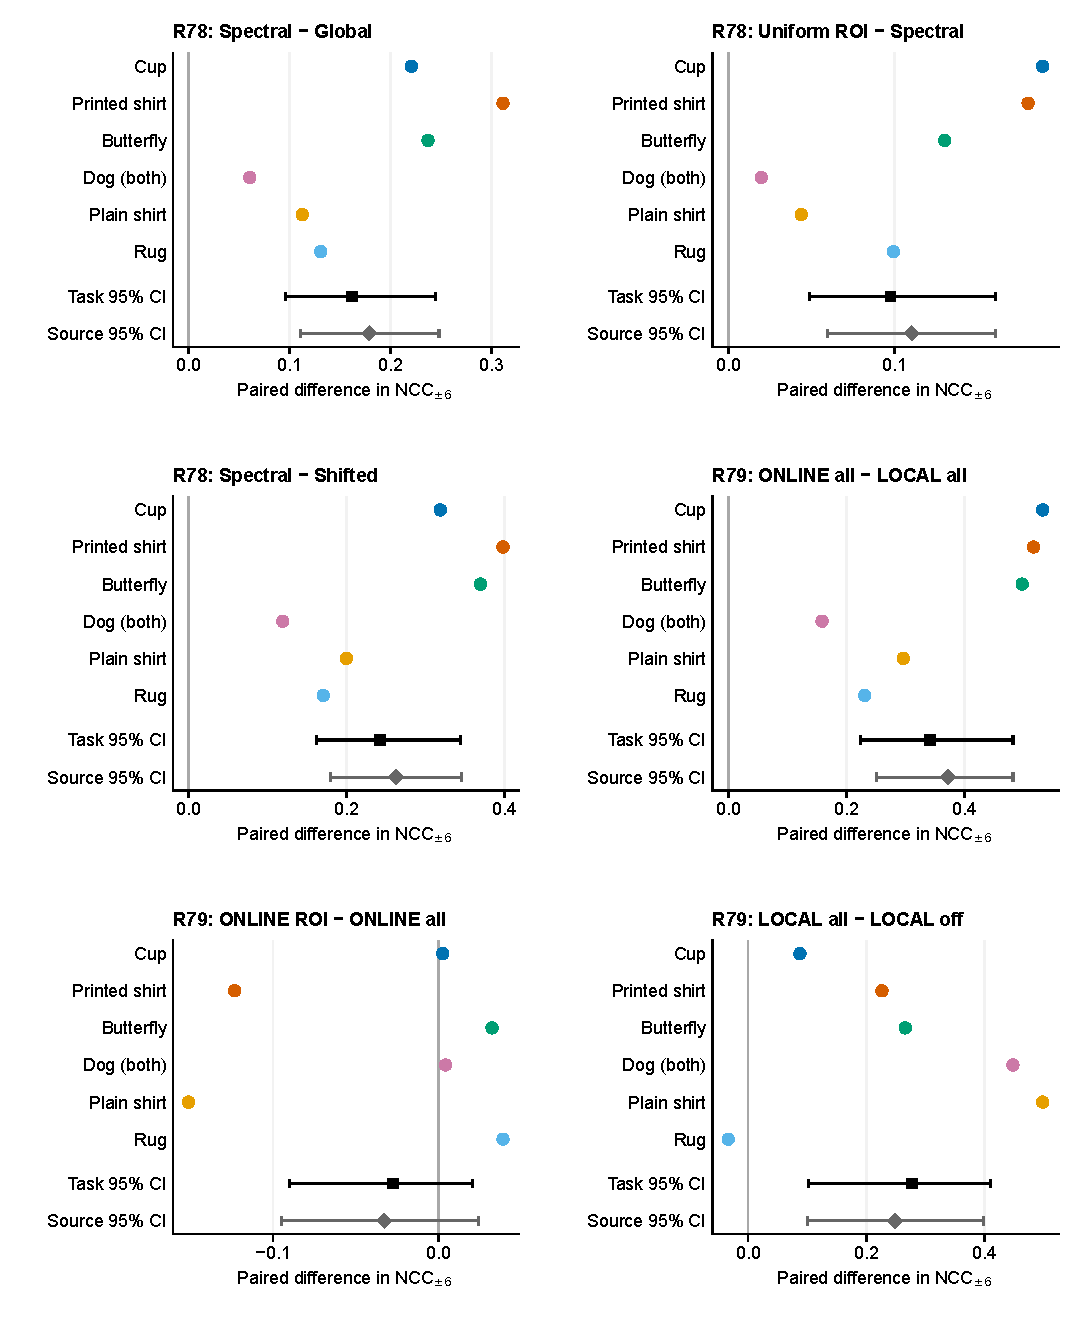
\includegraphics[width=\linewidth]{figures/evidence_paired_ncc.pdf}\caption{Source-level paired differences in shift-tolerant local NCC. Each colored point averages seeds and, for dog, both tasks. Squares and diamonds show task-weighted and source-weighted estimates with paired source-cluster bootstrap 95\% intervals. Differences follow the panel titles.}\label{fig:evidence-paired_ncc}\end{figure}

\begin{figure}[htbp]\centering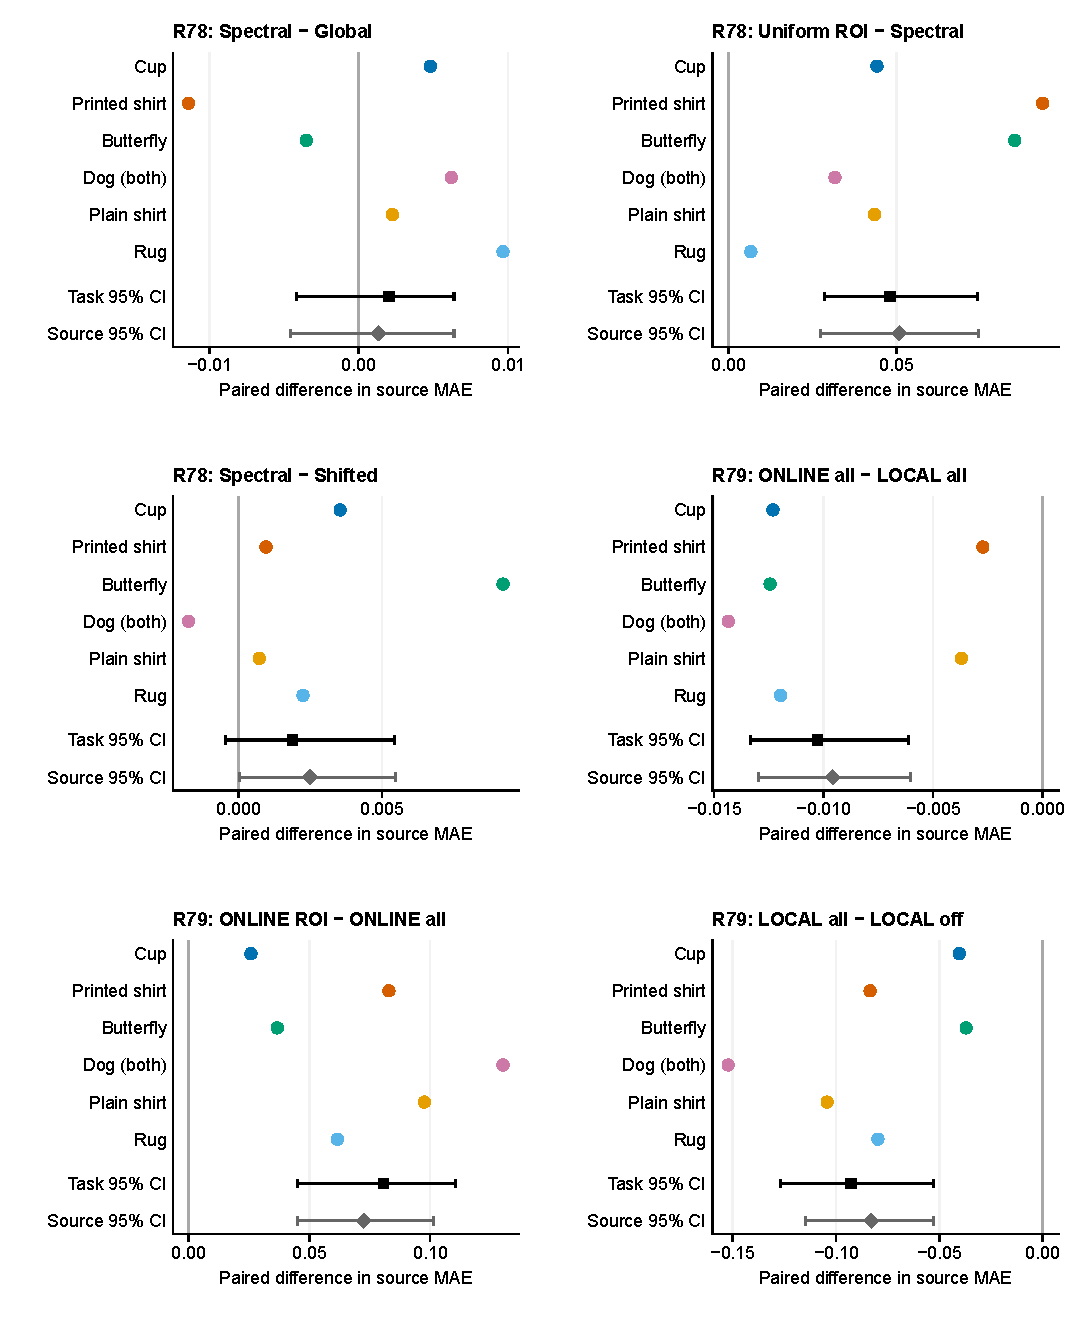
\includegraphics[width=\linewidth]{figures/evidence_paired_mae.pdf}\caption{Source-level paired differences in whole-image source MAE, with the same pairing and weights as the NCC plot. A positive difference means greater departure from the source image.}\label{fig:evidence-paired_mae}\end{figure}

\begin{figure}[htbp]\centering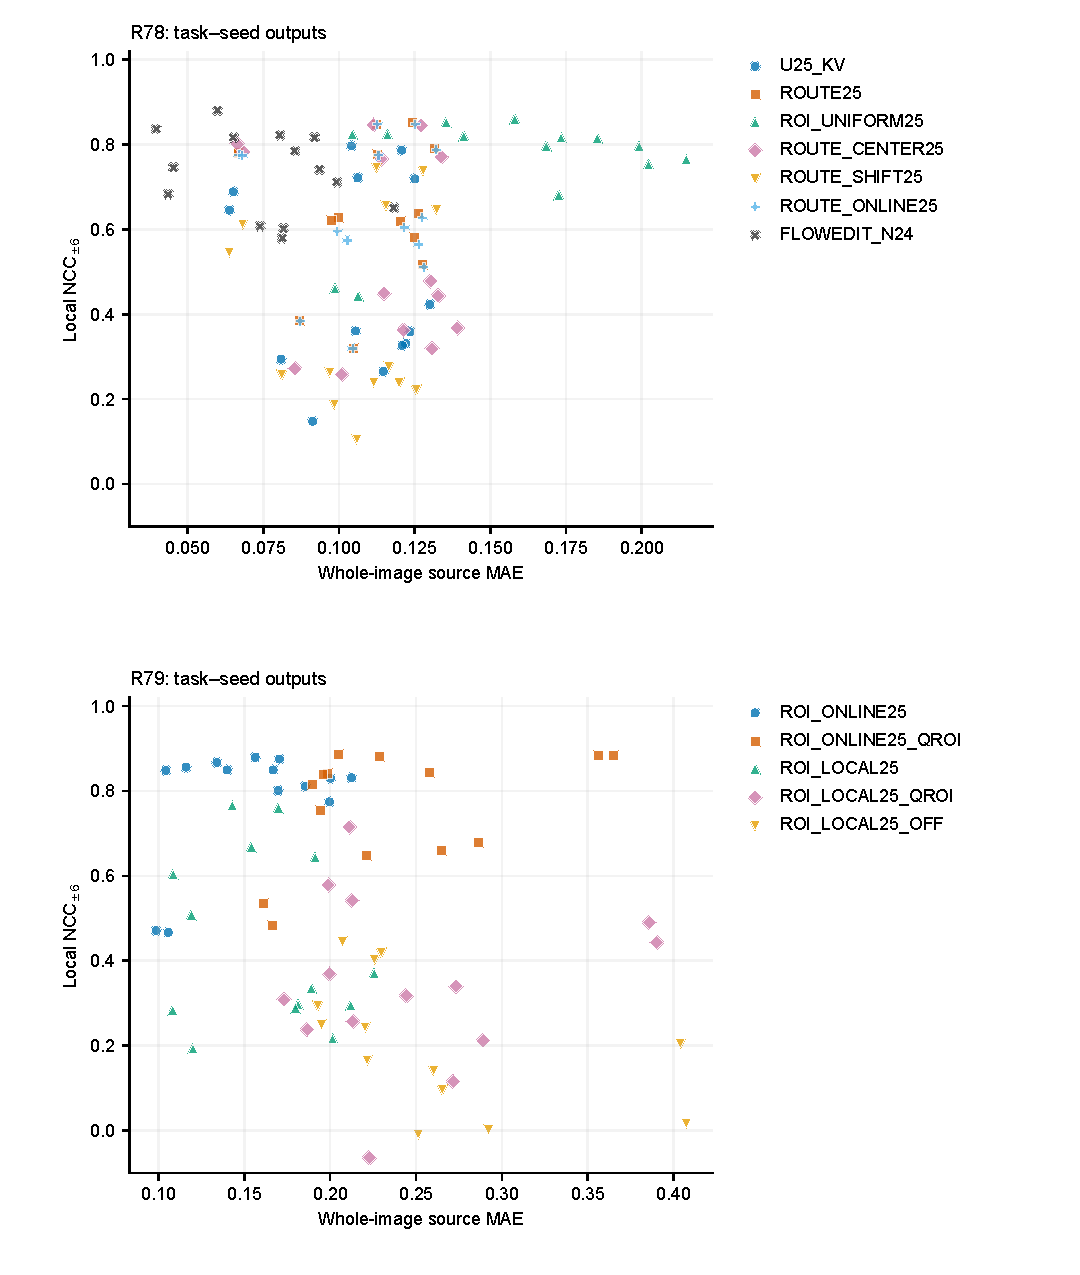
\includegraphics[width=\linewidth]{figures/evidence_ncc_source_mae_scatter.pdf}\caption{Local NCC versus whole-image source MAE for every completed task--seed output (98 R78, 70 R79). Colors and markers identify the recorded arms. Outputs sharing sources are dependent; these axes describe source correlation and source departure.}\label{fig:evidence-ncc_source_mae_scatter}\end{figure}

\subsection{Complete task-by-arm means and seed-level results}

Task codes: C = cup\_night; P = printed\_shirt\_studio; B = butterfly\_sunset; DS = dog\_snow; DR = dog\_rain; S = shirt\_studio; R = rug\_floor. Each task-by-arm row averages exactly two seeds. $I$ is the logged integrated correction impulse; a dash denotes an unavailable value. CSV exports retain the full precision and all original metric fields.

\begingroup\scriptsize\setlength{\tabcolsep}{2pt}
\begin{longtable}{lp{.29\linewidth}lrrrr}
\caption{All-arm aggregate means under both weighting rules. Each arm has 14 outputs, seven tasks, and six source clusters.}\\
\hline
Study & Arm & Weight & MAE & Fixed NCC & NCC$_{\pm6}$ & $I$ \\ \hline
\endfirsthead
\hline
Study & Arm & Weight & MAE & Fixed NCC & NCC$_{\pm6}$ & $I$ \\ \hline
\endhead
R78 & U25\_KV & Task & 0.1053 & 0.4799 & 0.4901 & 0.2260 \\
R78 & U25\_KV & Source & 0.1038 & 0.4365 & 0.4459 & 0.2258 \\
R78 & ROUTE25 & Task & 0.1073 & 0.6469 & 0.6521 & 0.2260 \\
R78 & ROUTE25 & Source & 0.1052 & 0.6196 & 0.6247 & 0.2258 \\
R78 & ROI\_UNIFORM25 & Task & 0.1554 & 0.7479 & 0.7496 & 0.2260 \\
R78 & ROI\_UNIFORM25 & Source & 0.1560 & 0.7339 & 0.7352 & 0.2258 \\
R78 & ROUTE\_CENTER25 & Task & 0.1126 & 0.5506 & 0.5542 & 0.2260 \\
R78 & ROUTE\_CENTER25 & Source & 0.1111 & 0.5092 & 0.5121 & 0.2258 \\
R78 & ROUTE\_SHIFT25 & Task & 0.1054 & 0.3923 & 0.4098 & 0.2260 \\
R78 & ROUTE\_SHIFT25 & Source & 0.1027 & 0.3456 & 0.3619 & 0.2258 \\
R78 & ROUTE\_ONLINE25 & Task & 0.1083 & 0.6369 & 0.6416 & 0.2221 \\
R78 & ROUTE\_ONLINE25 & Source & 0.1062 & 0.6084 & 0.6129 & 0.2217 \\
R78 & FLOWEDIT\_N24 & Task & 0.0757 & 0.7322 & 0.7339 & -- \\
R78 & FLOWEDIT\_N24 & Source & 0.0734 & 0.7245 & 0.7256 & -- \\
R79 & ROI\_ONLINE25 & Task & 0.1543 & 0.7857 & 0.7864 & 0.2524 \\
R79 & ROI\_ONLINE25 & Source & 0.1549 & 0.7722 & 0.7729 & 0.2513 \\
R79 & ROI\_ONLINE25\_QROI & Task & 0.2350 & 0.7538 & 0.7592 & 0.3046 \\
R79 & ROI\_ONLINE25\_QROI & Source & 0.2274 & 0.7341 & 0.7403 & 0.2994 \\
R79 & ROI\_LOCAL25 & Task & 0.1645 & 0.4319 & 0.4445 & 0.0921 \\
R79 & ROI\_LOCAL25 & Source & 0.1645 & 0.3906 & 0.4004 & 0.0881 \\
R79 & ROI\_LOCAL25\_QROI & Task & 0.2481 & 0.3164 & 0.3473 & 0.0945 \\
R79 & ROI\_LOCAL25\_QROI & Source & 0.2394 & 0.2835 & 0.3140 & 0.0900 \\
R79 & ROI\_LOCAL25\_OFF & Task & 0.2573 & 0.1478 & 0.1674 & 0.1015 \\
R79 & ROI\_LOCAL25\_OFF & Source & 0.2474 & 0.1327 & 0.1518 & 0.0970 \\
\hline\end{longtable}
\endgroup

\begingroup\scriptsize\setlength{\tabcolsep}{2pt}
\begin{longtable}{lp{.30\linewidth}rrrr}
\caption{R78 complete task-by-arm means ($n=2$ seeds each).}\\
\hline
Task & Recorded arm & MAE & Fixed NCC & NCC$_{\pm6}$ & $I$ \\ \hline
\endfirsthead
\hline
Task & Recorded arm & MAE & Fixed NCC & NCC$_{\pm6}$ & $I$ \\ \hline
\endhead
C & U25\_KV & 0.1215 & 0.3284 & 0.3284 & 0.2414 \\
C & ROUTE25 & 0.1263 & 0.5489 & 0.5489 & 0.2414 \\
C & ROI\_UNIFORM25 & 0.1705 & 0.7380 & 0.7380 & 0.2414 \\
C & ROUTE\_CENTER25 & 0.1316 & 0.4605 & 0.4605 & 0.2414 \\
C & ROUTE\_SHIFT25 & 0.1227 & 0.2217 & 0.2301 & 0.2414 \\
C & ROUTE\_ONLINE25 & 0.1273 & 0.5375 & 0.5375 & 0.2379 \\
C & FLOWEDIT\_N24 & 0.1059 & 0.6960 & 0.6960 & -- \\
P & U25\_KV & 0.1101 & 0.3118 & 0.3127 & 0.2262 \\
P & ROUTE25 & 0.0987 & 0.6240 & 0.6240 & 0.2262 \\
P & ROI\_UNIFORM25 & 0.1923 & 0.8043 & 0.8043 & 0.2262 \\
P & ROUTE\_CENTER25 & 0.1181 & 0.4059 & 0.4059 & 0.2262 \\
P & ROUTE\_SHIFT25 & 0.0978 & 0.2185 & 0.2257 & 0.2262 \\
P & ROUTE\_ONLINE25 & 0.1011 & 0.5844 & 0.5844 & 0.2165 \\
P & FLOWEDIT\_N24 & 0.0695 & 0.7121 & 0.7121 & -- \\
B & U25\_KV & 0.1268 & 0.3907 & 0.3907 & 0.2387 \\
B & ROUTE25 & 0.1232 & 0.6278 & 0.6278 & 0.2387 \\
B & ROI\_UNIFORM25 & 0.2085 & 0.7579 & 0.7579 & 0.2387 \\
B & ROUTE\_CENTER25 & 0.1349 & 0.3428 & 0.3428 & 0.2387 \\
B & ROUTE\_SHIFT25 & 0.1140 & 0.2383 & 0.2579 & 0.2387 \\
B & ROUTE\_ONLINE25 & 0.1245 & 0.6155 & 0.6155 & 0.2332 \\
B & FLOWEDIT\_N24 & 0.0815 & 0.5904 & 0.5904 & -- \\
DS & U25\_KV & 0.1229 & 0.7354 & 0.7526 & 0.2285 \\
DS & ROUTE25 & 0.1279 & 0.8135 & 0.8213 & 0.2285 \\
DS & ROI\_UNIFORM25 & 0.1657 & 0.8321 & 0.8373 & 0.2285 \\
DS & ROUTE\_CENTER25 & 0.1305 & 0.7982 & 0.8075 & 0.2285 \\
DS & ROUTE\_SHIFT25 & 0.1300 & 0.6662 & 0.6927 & 0.2285 \\
DS & ROUTE\_ONLINE25 & 0.1286 & 0.8092 & 0.8172 & 0.2256 \\
DS & FLOWEDIT\_N24 & 0.0956 & 0.7537 & 0.7634 & -- \\
DR & U25\_KV & 0.1052 & 0.7459 & 0.7589 & 0.2253 \\
DR & ROUTE25 & 0.1127 & 0.8078 & 0.8117 & 0.2253 \\
DR & ROI\_UNIFORM25 & 0.1383 & 0.8314 & 0.8355 & 0.2253 \\
DR & ROUTE\_CENTER25 & 0.1127 & 0.8009 & 0.8056 & 0.2253 \\
DR & ROUTE\_SHIFT25 & 0.1140 & 0.6795 & 0.7014 & 0.2253 \\
DR & ROUTE\_ONLINE25 & 0.1129 & 0.8068 & 0.8108 & 0.2238 \\
DR & FLOWEDIT\_N24 & 0.0829 & 0.8025 & 0.8032 & -- \\
S & U25\_KV & 0.0645 & 0.6375 & 0.6667 & 0.2144 \\
S & ROUTE25 & 0.0667 & 0.7544 & 0.7792 & 0.2144 \\
S & ROI\_UNIFORM25 & 0.1102 & 0.8203 & 0.8231 & 0.2144 \\
S & ROUTE\_CENTER25 & 0.0675 & 0.7859 & 0.7920 & 0.2144 \\
S & ROUTE\_SHIFT25 & 0.0660 & 0.5452 & 0.5793 & 0.2144 \\
S & ROUTE\_ONLINE25 & 0.0675 & 0.7535 & 0.7745 & 0.2111 \\
S & FLOWEDIT\_N24 & 0.0498 & 0.8568 & 0.8581 & -- \\
R & U25\_KV & 0.0861 & 0.2097 & 0.2209 & 0.2074 \\
R & ROUTE25 & 0.0958 & 0.3519 & 0.3519 & 0.2074 \\
R & ROI\_UNIFORM25 & 0.1025 & 0.4512 & 0.4512 & 0.2074 \\
R & ROUTE\_CENTER25 & 0.0932 & 0.2601 & 0.2648 & 0.2074 \\
R & ROUTE\_SHIFT25 & 0.0935 & 0.1768 & 0.1814 & 0.2074 \\
R & ROUTE\_ONLINE25 & 0.0959 & 0.3515 & 0.3515 & 0.2065 \\
R & FLOWEDIT\_N24 & 0.0445 & 0.7139 & 0.7139 & -- \\
\hline\end{longtable}
\endgroup

\begingroup\scriptsize\setlength{\tabcolsep}{2pt}
\begin{longtable}{llp{.29\linewidth}rrrr}
\caption{R78 complete per-seed quantitative results.}\\
\hline
Task & Seed & Recorded arm & MAE & Fixed NCC & NCC$_{\pm6}$ & $I$ \\ \hline
\endfirsthead
\hline
Task & Seed & Recorded arm & MAE & Fixed NCC & NCC$_{\pm6}$ & $I$ \\ \hline
\endhead
C & 10 & U25\_KV & 0.1220 & 0.3307 & 0.3307 & 0.2422 \\
C & 17 & U25\_KV & 0.1209 & 0.3261 & 0.3261 & 0.2406 \\
C & 10 & ROUTE25 & 0.1250 & 0.5799 & 0.5799 & 0.2422 \\
C & 17 & ROUTE25 & 0.1275 & 0.5180 & 0.5180 & 0.2406 \\
C & 10 & ROI\_UNIFORM25 & 0.1684 & 0.7957 & 0.7957 & 0.2422 \\
C & 17 & ROI\_UNIFORM25 & 0.1726 & 0.6803 & 0.6803 & 0.2406 \\
C & 10 & ROUTE\_CENTER25 & 0.1328 & 0.4432 & 0.4432 & 0.2422 \\
C & 17 & ROUTE\_CENTER25 & 0.1303 & 0.4778 & 0.4778 & 0.2406 \\
C & 10 & ROUTE\_SHIFT25 & 0.1199 & 0.2339 & 0.2381 & 0.2422 \\
C & 17 & ROUTE\_SHIFT25 & 0.1255 & 0.2094 & 0.2221 & 0.2406 \\
C & 10 & ROUTE\_ONLINE25 & 0.1264 & 0.5642 & 0.5642 & 0.2376 \\
C & 17 & ROUTE\_ONLINE25 & 0.1281 & 0.5108 & 0.5108 & 0.2382 \\
C & 10 & FLOWEDIT\_N24 & 0.1181 & 0.6503 & 0.6503 & -- \\
C & 17 & FLOWEDIT\_N24 & 0.0936 & 0.7416 & 0.7416 & -- \\
P & 0 & U25\_KV & 0.1147 & 0.2651 & 0.2651 & 0.2280 \\
P & 17 & U25\_KV & 0.1055 & 0.3586 & 0.3604 & 0.2245 \\
P & 0 & ROUTE25 & 0.0998 & 0.6279 & 0.6279 & 0.2280 \\
P & 17 & ROUTE25 & 0.0977 & 0.6201 & 0.6201 & 0.2245 \\
P & 0 & ROI\_UNIFORM25 & 0.1991 & 0.7947 & 0.7947 & 0.2280 \\
P & 17 & ROI\_UNIFORM25 & 0.1854 & 0.8139 & 0.8139 & 0.2245 \\
P & 0 & ROUTE\_CENTER25 & 0.1213 & 0.3623 & 0.3623 & 0.2280 \\
P & 17 & ROUTE\_CENTER25 & 0.1149 & 0.4495 & 0.4495 & 0.2245 \\
P & 0 & ROUTE\_SHIFT25 & 0.0985 & 0.1761 & 0.1879 & 0.2280 \\
P & 17 & ROUTE\_SHIFT25 & 0.0970 & 0.2609 & 0.2634 & 0.2245 \\
P & 0 & ROUTE\_ONLINE25 & 0.1029 & 0.5735 & 0.5735 & 0.2167 \\
P & 17 & ROUTE\_ONLINE25 & 0.0994 & 0.5953 & 0.5953 & 0.2164 \\
P & 0 & FLOWEDIT\_N24 & 0.0651 & 0.8168 & 0.8168 & -- \\
P & 17 & FLOWEDIT\_N24 & 0.0740 & 0.6074 & 0.6074 & -- \\
B & 0 & U25\_KV & 0.1300 & 0.4229 & 0.4229 & 0.2425 \\
B & 17 & U25\_KV & 0.1235 & 0.3585 & 0.3585 & 0.2348 \\
B & 0 & ROUTE25 & 0.1262 & 0.6380 & 0.6380 & 0.2425 \\
B & 17 & ROUTE25 & 0.1203 & 0.6175 & 0.6175 & 0.2348 \\
B & 0 & ROI\_UNIFORM25 & 0.2147 & 0.7638 & 0.7638 & 0.2425 \\
B & 17 & ROI\_UNIFORM25 & 0.2022 & 0.7520 & 0.7520 & 0.2348 \\
B & 0 & ROUTE\_CENTER25 & 0.1390 & 0.3675 & 0.3675 & 0.2425 \\
B & 17 & ROUTE\_CENTER25 & 0.1308 & 0.3182 & 0.3182 & 0.2348 \\
B & 0 & ROUTE\_SHIFT25 & 0.1165 & 0.2755 & 0.2766 & 0.2425 \\
B & 17 & ROUTE\_SHIFT25 & 0.1115 & 0.2012 & 0.2392 & 0.2348 \\
B & 0 & ROUTE\_ONLINE25 & 0.1275 & 0.6272 & 0.6272 & 0.2372 \\
B & 17 & ROUTE\_ONLINE25 & 0.1215 & 0.6039 & 0.6039 & 0.2293 \\
B & 0 & FLOWEDIT\_N24 & 0.0813 & 0.5793 & 0.5793 & -- \\
B & 17 & FLOWEDIT\_N24 & 0.0817 & 0.6015 & 0.6015 & -- \\
DS & 0 & U25\_KV & 0.1208 & 0.7829 & 0.7865 & 0.2285 \\
DS & 17 & U25\_KV & 0.1251 & 0.6880 & 0.7188 & 0.2285 \\
DS & 0 & ROUTE25 & 0.1243 & 0.8510 & 0.8520 & 0.2285 \\
DS & 17 & ROUTE25 & 0.1314 & 0.7760 & 0.7907 & 0.2285 \\
DS & 0 & ROI\_UNIFORM25 & 0.1581 & 0.8579 & 0.8594 & 0.2285 \\
DS & 17 & ROI\_UNIFORM25 & 0.1734 & 0.8064 & 0.8151 & 0.2285 \\
DS & 0 & ROUTE\_CENTER25 & 0.1271 & 0.8427 & 0.8445 & 0.2285 \\
DS & 17 & ROUTE\_CENTER25 & 0.1338 & 0.7537 & 0.7706 & 0.2285 \\
DS & 0 & ROUTE\_SHIFT25 & 0.1278 & 0.7312 & 0.7387 & 0.2285 \\
DS & 17 & ROUTE\_SHIFT25 & 0.1322 & 0.6013 & 0.6467 & 0.2285 \\
DS & 0 & ROUTE\_ONLINE25 & 0.1252 & 0.8459 & 0.8474 & 0.2246 \\
DS & 17 & ROUTE\_ONLINE25 & 0.1321 & 0.7726 & 0.7871 & 0.2267 \\
DS & 0 & FLOWEDIT\_N24 & 0.0993 & 0.6919 & 0.7111 & -- \\
DS & 17 & FLOWEDIT\_N24 & 0.0919 & 0.8156 & 0.8156 & -- \\
DR & 0 & U25\_KV & 0.1041 & 0.7929 & 0.7964 & 0.2254 \\
DR & 17 & U25\_KV & 0.1063 & 0.6989 & 0.7215 & 0.2253 \\
DR & 0 & ROUTE25 & 0.1124 & 0.8456 & 0.8477 & 0.2254 \\
DR & 17 & ROUTE25 & 0.1129 & 0.7701 & 0.7756 & 0.2253 \\
DR & 0 & ROI\_UNIFORM25 & 0.1354 & 0.8496 & 0.8516 & 0.2254 \\
DR & 17 & ROI\_UNIFORM25 & 0.1412 & 0.8133 & 0.8194 & 0.2253 \\
DR & 0 & ROUTE\_CENTER25 & 0.1114 & 0.8442 & 0.8460 & 0.2254 \\
DR & 17 & ROUTE\_CENTER25 & 0.1140 & 0.7576 & 0.7653 & 0.2253 \\
DR & 0 & ROUTE\_SHIFT25 & 0.1124 & 0.7378 & 0.7461 & 0.2254 \\
DR & 17 & ROUTE\_SHIFT25 & 0.1155 & 0.6212 & 0.6567 & 0.2253 \\
DR & 0 & ROUTE\_ONLINE25 & 0.1126 & 0.8452 & 0.8474 & 0.2242 \\
DR & 17 & ROUTE\_ONLINE25 & 0.1131 & 0.7684 & 0.7743 & 0.2234 \\
DR & 0 & FLOWEDIT\_N24 & 0.0854 & 0.7830 & 0.7844 & -- \\
DR & 17 & FLOWEDIT\_N24 & 0.0805 & 0.8220 & 0.8220 & -- \\
S & 0 & U25\_KV & 0.0638 & 0.6269 & 0.6451 & 0.2134 \\
S & 17 & U25\_KV & 0.0651 & 0.6481 & 0.6883 & 0.2154 \\
S & 0 & ROUTE25 & 0.0667 & 0.7781 & 0.7781 & 0.2134 \\
S & 17 & ROUTE25 & 0.0668 & 0.7306 & 0.7803 & 0.2154 \\
S & 0 & ROI\_UNIFORM25 & 0.1161 & 0.8226 & 0.8226 & 0.2134 \\
S & 17 & ROI\_UNIFORM25 & 0.1044 & 0.8180 & 0.8236 & 0.2154 \\
S & 0 & ROUTE\_CENTER25 & 0.0664 & 0.7978 & 0.8017 & 0.2134 \\
S & 17 & ROUTE\_CENTER25 & 0.0686 & 0.7741 & 0.7823 & 0.2154 \\
S & 0 & ROUTE\_SHIFT25 & 0.0638 & 0.5244 & 0.5464 & 0.2134 \\
S & 17 & ROUTE\_SHIFT25 & 0.0682 & 0.5659 & 0.6123 & 0.2154 \\
S & 0 & ROUTE\_ONLINE25 & 0.0670 & 0.7754 & 0.7754 & 0.2114 \\
S & 17 & ROUTE\_ONLINE25 & 0.0681 & 0.7317 & 0.7737 & 0.2109 \\
S & 0 & FLOWEDIT\_N24 & 0.0396 & 0.8355 & 0.8362 & -- \\
S & 17 & FLOWEDIT\_N24 & 0.0599 & 0.8781 & 0.8800 & -- \\
R & 0 & U25\_KV & 0.0809 & 0.2716 & 0.2939 & 0.2055 \\
R & 17 & U25\_KV & 0.0913 & 0.1479 & 0.1479 & 0.2094 \\
R & 0 & ROUTE25 & 0.0869 & 0.3853 & 0.3853 & 0.2055 \\
R & 17 & ROUTE25 & 0.1047 & 0.3184 & 0.3184 & 0.2094 \\
R & 0 & ROI\_UNIFORM25 & 0.0987 & 0.4598 & 0.4598 & 0.2055 \\
R & 17 & ROI\_UNIFORM25 & 0.1063 & 0.4426 & 0.4426 & 0.2094 \\
R & 0 & ROUTE\_CENTER25 & 0.0854 & 0.2624 & 0.2718 & 0.2055 \\
R & 17 & ROUTE\_CENTER25 & 0.1010 & 0.2578 & 0.2578 & 0.2094 \\
R & 0 & ROUTE\_SHIFT25 & 0.0811 & 0.2562 & 0.2568 & 0.2055 \\
R & 17 & ROUTE\_SHIFT25 & 0.1059 & 0.0974 & 0.1059 & 0.2094 \\
R & 0 & ROUTE\_ONLINE25 & 0.0872 & 0.3838 & 0.3838 & 0.2035 \\
R & 17 & ROUTE\_ONLINE25 & 0.1046 & 0.3191 & 0.3191 & 0.2096 \\
R & 0 & FLOWEDIT\_N24 & 0.0436 & 0.6823 & 0.6823 & -- \\
R & 17 & FLOWEDIT\_N24 & 0.0454 & 0.7454 & 0.7454 & -- \\
\hline\end{longtable}
\endgroup

\begingroup\scriptsize\setlength{\tabcolsep}{2pt}
\begin{longtable}{lp{.30\linewidth}rrrr}
\caption{R79 complete task-by-arm means ($n=2$ seeds each).}\\
\hline
Task & Recorded arm & MAE & Fixed NCC & NCC$_{\pm6}$ & $I$ \\ \hline
\endfirsthead
\hline
Task & Recorded arm & MAE & Fixed NCC & NCC$_{\pm6}$ & $I$ \\ \hline
\endhead
C & ROI\_ONLINE25 & 0.1683 & 0.8252 & 0.8252 & 0.2649 \\
C & ROI\_ONLINE25\_QROI & 0.1941 & 0.8280 & 0.8280 & 0.2842 \\
C & ROI\_LOCAL25 & 0.1806 & 0.2924 & 0.2924 & 0.0984 \\
C & ROI\_LOCAL25\_QROI & 0.2064 & 0.3121 & 0.3132 & 0.0993 \\
C & ROI\_LOCAL25\_OFF & 0.2209 & 0.2023 & 0.2049 & 0.1069 \\
P & ROI\_ONLINE25 & 0.1925 & 0.7927 & 0.7927 & 0.2588 \\
P & ROI\_ONLINE25\_QROI & 0.2755 & 0.6696 & 0.6696 & 0.3165 \\
P & ROI\_LOCAL25 & 0.1953 & 0.2739 & 0.2754 & 0.0571 \\
P & ROI\_LOCAL25\_QROI & 0.2804 & 0.0977 & 0.1637 & 0.0592 \\
P & ROI\_LOCAL25\_OFF & 0.2787 & 0.0208 & 0.0491 & 0.0665 \\
B & ROI\_ONLINE25 & 0.2063 & 0.8304 & 0.8304 & 0.2734 \\
B & ROI\_ONLINE25\_QROI & 0.2430 & 0.8630 & 0.8630 & 0.2928 \\
B & ROI\_LOCAL25 & 0.2187 & 0.3324 & 0.3324 & 0.0825 \\
B & ROI\_LOCAL25\_QROI & 0.2589 & 0.3241 & 0.3289 & 0.0800 \\
B & ROI\_LOCAL25\_OFF & 0.2557 & 0.0547 & 0.0667 & 0.0922 \\
DS & ROI\_ONLINE25 & 0.1634 & 0.8763 & 0.8772 & 0.2612 \\
DS & ROI\_ONLINE25\_QROI & 0.3605 & 0.8824 & 0.8825 & 0.3930 \\
DS & ROI\_LOCAL25 & 0.1806 & 0.6723 & 0.7010 & 0.1179 \\
DS & ROI\_LOCAL25\_QROI & 0.3880 & 0.4314 & 0.4664 & 0.1301 \\
DS & ROI\_LOCAL25\_OFF & 0.4056 & 0.0824 & 0.1112 & 0.1390 \\
DR & ROI\_ONLINE25 & 0.1370 & 0.8571 & 0.8583 & 0.2570 \\
DR & ROI\_ONLINE25\_QROI & 0.2002 & 0.8619 & 0.8619 & 0.2793 \\
DR & ROI\_LOCAL25 & 0.1486 & 0.6877 & 0.7165 & 0.1131 \\
DR & ROI\_LOCAL25\_QROI & 0.2120 & 0.5962 & 0.6284 & 0.1129 \\
DR & ROI\_LOCAL25\_OFF & 0.2278 & 0.3935 & 0.4109 & 0.1174 \\
S & ROI\_ONLINE25 & 0.1102 & 0.8491 & 0.8522 & 0.2385 \\
S & ROI\_ONLINE25\_QROI & 0.2078 & 0.6636 & 0.7012 & 0.3176 \\
S & ROI\_LOCAL25 & 0.1139 & 0.5273 & 0.5557 & 0.0743 \\
S & ROI\_LOCAL25\_QROI & 0.2109 & 0.1803 & 0.2575 & 0.0750 \\
S & ROI\_LOCAL25\_OFF & 0.2182 & 0.0109 & 0.0577 & 0.0801 \\
R & ROI\_ONLINE25 & 0.1022 & 0.4689 & 0.4689 & 0.2131 \\
R & ROI\_ONLINE25\_QROI & 0.1638 & 0.5081 & 0.5081 & 0.2489 \\
R & ROI\_LOCAL25 & 0.1141 & 0.2373 & 0.2378 & 0.1011 \\
R & ROI\_LOCAL25\_QROI & 0.1799 & 0.2731 & 0.2731 & 0.1049 \\
R & ROI\_LOCAL25\_OFF & 0.1939 & 0.2699 & 0.2714 & 0.1082 \\
\hline\end{longtable}
\endgroup

\begingroup\scriptsize\setlength{\tabcolsep}{2pt}
\begin{longtable}{llp{.29\linewidth}rrrr}
\caption{R79 complete per-seed quantitative results.}\\
\hline
Task & Seed & Recorded arm & MAE & Fixed NCC & NCC$_{\pm6}$ & $I$ \\ \hline
\endfirsthead
\hline
Task & Seed & Recorded arm & MAE & Fixed NCC & NCC$_{\pm6}$ & $I$ \\ \hline
\endhead
C & 10 & ROI\_ONLINE25 & 0.1668 & 0.8495 & 0.8495 & 0.2623 \\
C & 17 & ROI\_ONLINE25 & 0.1697 & 0.8009 & 0.8009 & 0.2676 \\
C & 10 & ROI\_ONLINE25\_QROI & 0.1983 & 0.8404 & 0.8404 & 0.2834 \\
C & 17 & ROI\_ONLINE25\_QROI & 0.1899 & 0.8155 & 0.8155 & 0.2850 \\
C & 10 & ROI\_LOCAL25 & 0.1813 & 0.2966 & 0.2966 & 0.0971 \\
C & 17 & ROI\_LOCAL25 & 0.1798 & 0.2883 & 0.2883 & 0.0997 \\
C & 10 & ROI\_LOCAL25\_QROI & 0.2131 & 0.2548 & 0.2569 & 0.0989 \\
C & 17 & ROI\_LOCAL25\_QROI & 0.1997 & 0.3694 & 0.3694 & 0.0996 \\
C & 10 & ROI\_LOCAL25\_OFF & 0.2215 & 0.1609 & 0.1660 & 0.1073 \\
C & 17 & ROI\_LOCAL25\_OFF & 0.2204 & 0.2438 & 0.2438 & 0.1066 \\
P & 0 & ROI\_ONLINE25 & 0.1995 & 0.7743 & 0.7743 & 0.2636 \\
P & 17 & ROI\_ONLINE25 & 0.1855 & 0.8110 & 0.8110 & 0.2541 \\
P & 0 & ROI\_ONLINE25\_QROI & 0.2647 & 0.6603 & 0.6603 & 0.3138 \\
P & 17 & ROI\_ONLINE25\_QROI & 0.2862 & 0.6788 & 0.6788 & 0.3192 \\
P & 0 & ROI\_LOCAL25 & 0.2014 & 0.2129 & 0.2160 & 0.0559 \\
P & 17 & ROI\_LOCAL25 & 0.1891 & 0.3348 & 0.3348 & 0.0583 \\
P & 0 & ROI\_LOCAL25\_QROI & 0.2717 & 0.0068 & 0.1154 & 0.0632 \\
P & 17 & ROI\_LOCAL25\_QROI & 0.2890 & 0.1886 & 0.2120 & 0.0551 \\
P & 0 & ROI\_LOCAL25\_OFF & 0.2653 & 0.0472 & 0.0963 & 0.0651 \\
P & 17 & ROI\_LOCAL25\_OFF & 0.2922 & -0.0057 & 0.0019 & 0.0679 \\
B & 0 & ROI\_ONLINE25 & 0.2124 & 0.8312 & 0.8312 & 0.2783 \\
B & 17 & ROI\_ONLINE25 & 0.2002 & 0.8297 & 0.8297 & 0.2685 \\
B & 0 & ROI\_ONLINE25\_QROI & 0.2576 & 0.8437 & 0.8437 & 0.3006 \\
B & 17 & ROI\_ONLINE25\_QROI & 0.2285 & 0.8823 & 0.8823 & 0.2850 \\
B & 0 & ROI\_LOCAL25 & 0.2256 & 0.3698 & 0.3698 & 0.0825 \\
B & 17 & ROI\_LOCAL25 & 0.2119 & 0.2950 & 0.2950 & 0.0825 \\
B & 0 & ROI\_LOCAL25\_QROI & 0.2733 & 0.3368 & 0.3397 & 0.0790 \\
B & 17 & ROI\_LOCAL25\_QROI & 0.2444 & 0.3114 & 0.3181 & 0.0810 \\
B & 0 & ROI\_LOCAL25\_OFF & 0.2602 & 0.1417 & 0.1417 & 0.0852 \\
B & 17 & ROI\_LOCAL25\_OFF & 0.2513 & -0.0324 & -0.0083 & 0.0993 \\
DS & 0 & ROI\_ONLINE25 & 0.1563 & 0.8792 & 0.8792 & 0.2555 \\
DS & 17 & ROI\_ONLINE25 & 0.1704 & 0.8733 & 0.8752 & 0.2668 \\
DS & 0 & ROI\_ONLINE25\_QROI & 0.3647 & 0.8825 & 0.8825 & 0.3955 \\
DS & 17 & ROI\_ONLINE25\_QROI & 0.3563 & 0.8822 & 0.8824 & 0.3905 \\
DS & 0 & ROI\_LOCAL25 & 0.1699 & 0.7512 & 0.7593 & 0.1095 \\
DS & 17 & ROI\_LOCAL25 & 0.1913 & 0.5933 & 0.6427 & 0.1264 \\
DS & 0 & ROI\_LOCAL25\_QROI & 0.3902 & 0.4420 & 0.4427 & 0.1309 \\
DS & 17 & ROI\_LOCAL25\_QROI & 0.3858 & 0.4207 & 0.4900 & 0.1294 \\
DS & 0 & ROI\_LOCAL25\_OFF & 0.4074 & -0.0200 & 0.0169 & 0.1438 \\
DS & 17 & ROI\_LOCAL25\_OFF & 0.4039 & 0.1847 & 0.2056 & 0.1341 \\
DR & 0 & ROI\_ONLINE25 & 0.1341 & 0.8662 & 0.8672 & 0.2509 \\
DR & 17 & ROI\_ONLINE25 & 0.1400 & 0.8480 & 0.8495 & 0.2630 \\
DR & 0 & ROI\_ONLINE25\_QROI & 0.2046 & 0.8847 & 0.8847 & 0.2834 \\
DR & 17 & ROI\_ONLINE25\_QROI & 0.1958 & 0.8391 & 0.8391 & 0.2753 \\
DR & 0 & ROI\_LOCAL25 & 0.1430 & 0.7584 & 0.7653 & 0.1055 \\
DR & 17 & ROI\_LOCAL25 & 0.1541 & 0.6170 & 0.6676 & 0.1207 \\
DR & 0 & ROI\_LOCAL25\_QROI & 0.2111 & 0.7136 & 0.7148 & 0.1062 \\
DR & 17 & ROI\_LOCAL25\_QROI & 0.2128 & 0.4788 & 0.5419 & 0.1196 \\
DR & 0 & ROI\_LOCAL25\_OFF & 0.2298 & 0.3927 & 0.4186 & 0.1147 \\
DR & 17 & ROI\_LOCAL25\_OFF & 0.2258 & 0.3942 & 0.4032 & 0.1201 \\
S & 0 & ROI\_ONLINE25 & 0.1161 & 0.8561 & 0.8561 & 0.2412 \\
S & 17 & ROI\_ONLINE25 & 0.1043 & 0.8421 & 0.8483 & 0.2357 \\
S & 0 & ROI\_ONLINE25\_QROI & 0.2210 & 0.5981 & 0.6487 & 0.3281 \\
S & 17 & ROI\_ONLINE25\_QROI & 0.1946 & 0.7292 & 0.7537 & 0.3071 \\
S & 0 & ROI\_LOCAL25 & 0.1192 & 0.4875 & 0.5077 & 0.0718 \\
S & 17 & ROI\_LOCAL25 & 0.1086 & 0.5671 & 0.6037 & 0.0768 \\
S & 0 & ROI\_LOCAL25\_QROI & 0.2229 & -0.1267 & -0.0635 & 0.0747 \\
S & 17 & ROI\_LOCAL25\_QROI & 0.1990 & 0.4874 & 0.5786 & 0.0754 \\
S & 0 & ROI\_LOCAL25\_OFF & 0.2292 & -0.3757 & -0.3294 & 0.0818 \\
S & 17 & ROI\_LOCAL25\_OFF & 0.2072 & 0.3974 & 0.4449 & 0.0784 \\
R & 0 & ROI\_ONLINE25 & 0.0987 & 0.4709 & 0.4709 & 0.2101 \\
R & 17 & ROI\_ONLINE25 & 0.1057 & 0.4669 & 0.4669 & 0.2161 \\
R & 0 & ROI\_ONLINE25\_QROI & 0.1610 & 0.5340 & 0.5340 & 0.2500 \\
R & 17 & ROI\_ONLINE25\_QROI & 0.1666 & 0.4823 & 0.4823 & 0.2478 \\
R & 0 & ROI\_LOCAL25 & 0.1082 & 0.2832 & 0.2832 & 0.0951 \\
R & 17 & ROI\_LOCAL25 & 0.1200 & 0.1915 & 0.1924 & 0.1070 \\
R & 0 & ROI\_LOCAL25\_QROI & 0.1731 & 0.3081 & 0.3081 & 0.1007 \\
R & 17 & ROI\_LOCAL25\_QROI & 0.1867 & 0.2382 & 0.2382 & 0.1092 \\
R & 0 & ROI\_LOCAL25\_OFF & 0.1928 & 0.2938 & 0.2940 & 0.1071 \\
R & 17 & ROI\_LOCAL25\_OFF & 0.1949 & 0.2460 & 0.2489 & 0.1092 \\
\hline\end{longtable}
\endgroup

\subsection{Recorded settings and computational cost}

The following settings and costs are read from the root metrics and per-output step summaries. Trace-based arms record 28 inversion evaluations and 28 integration steps. Memory-enabled editing records three evaluations at zero-based steps 0--6 and two at steps 7--27 (63 editing evaluations); LOCAL memory-off records two at every step (56). FlowEdit has no per-step records in these archives; its root metrics report 48 standalone evaluations and no inversion. The CSV step ledger contains every available step record rather than synthesizing absent FlowEdit records.

Standalone NFE charges the branch including inversion. Required NFE additionally charges a U25 prerequisite where the archive records an external budget. The four externally budgeted R78 branches each record 91 standalone and 182 required evaluations; this is a per-output prerequisite accounting, not the total of a batch with reference reuse. Synchronized seconds below are the actual logged branch measurements (mean and observed range over 14 outputs), with prerequisite execution excluded. Execution order, warmup, and hardware conditions are not controlled by these tables; seconds are not extrapolated from NFE.

\begingroup\scriptsize\setlength{\tabcolsep}{2pt}
\begin{longtable}{lp{.25\linewidth}rrrrrrp{.20\linewidth}}
\caption{Logged evaluation counts and synchronized branch time in seconds. Cur. and ref. are current-source and reference-source evaluations.}\\
\hline
Study & Arm & Inv. & Cur. & Ref. & Target & Branch & Required & Seconds: mean [min, max] \\ \hline
\endfirsthead
\hline
Study & Arm & Inv. & Cur. & Ref. & Target & Branch & Required & Seconds: mean [min, max] \\ \hline
\endhead
R78 & U25\_KV & 28 & 28 & 7 & 28 & 91 & 91 & 55.29 [43.99, 78.53] \\
R78 & ROUTE25 & 28 & 28 & 7 & 28 & 91 & 182 & 45.30 [42.44, 49.09] \\
R78 & ROI\_UNIFORM25 & 28 & 28 & 7 & 28 & 91 & 182 & 45.58 [42.62, 49.70] \\
R78 & ROUTE\_CENTER25 & 28 & 28 & 7 & 28 & 91 & 182 & 46.16 [44.02, 48.43] \\
R78 & ROUTE\_SHIFT25 & 28 & 28 & 7 & 28 & 91 & 182 & 45.37 [43.23, 48.95] \\
R78 & ROUTE\_ONLINE25 & 28 & 28 & 7 & 28 & 91 & 91 & 45.76 [43.62, 49.65] \\
R78 & FLOWEDIT\_N24 & 0 & -- & -- & 24 & 48 & 48 & 31.38 [29.76, 33.30] \\
R79 & ROI\_ONLINE25 & 28 & 28 & 7 & 28 & 91 & 91 & 54.07 [43.78, 78.61] \\
R79 & ROI\_ONLINE25\_QROI & 28 & 28 & 7 & 28 & 91 & 91 & 44.03 [42.93, 45.99] \\
R79 & ROI\_LOCAL25 & 28 & 28 & 7 & 28 & 91 & 91 & 44.93 [43.10, 47.11] \\
R79 & ROI\_LOCAL25\_QROI & 28 & 28 & 7 & 28 & 91 & 91 & 45.03 [43.66, 46.58] \\
R79 & ROI\_LOCAL25\_OFF & 28 & 28 & 0 & 28 & 84 & 84 & 40.89 [39.75, 42.06] \\
\hline\end{longtable}
\endgroup

\begingroup\scriptsize\setlength{\tabcolsep}{2pt}
\begin{longtable}{p{.46\linewidth}p{.46\linewidth}}
\caption{Recorded trace-arm settings. Nonempty values are shown; feathering applies to routed arms, spectral settings to spectral arms, and the KV pool token field is recorded in R79. Memory-off has zero active memory steps. Full per-output settings, ROI coordinates, and shifts are in the parameter CSV.}\\
\hline
Field & Recorded nonempty values \\ \hline
\endfirsthead
\hline
Field & Recorded nonempty values \\ \hline
\endhead
steps & 28 \\
resolution & 512 \\
guidance & 3.5 \\
gamma & 0.5 \\
eta & 0.0 \\
corr\_lambda & 0.25 \\
correction\_budget\_h & 0.25 \\
route\_feather\_px & 16.0 \\
global\_update & True \\
route\_changes\_update\_mask & False \\
memory\_pairing & paired \\
memory\_source\_k & True \\
memory\_source\_v & True \\
query\_write\_weight & 1.0; 0.0 \\
source\_kv\_pool\_tokens & 1024.0 \\
spectral\_kernel & 5.0 \\
spectral\_low\_weight & 0.5 \\
\hline\end{longtable}
\endgroup

\begingroup\scriptsize\setlength{\tabcolsep}{2pt}
\begin{longtable}{lp{.23\linewidth}p{.19\linewidth}p{.12\linewidth}p{.19\linewidth}l}
\caption{Arm-specific budget, shape, and query fields as recorded. A dash denotes an absent field. Trace memory windows are zero-based [0,7); memory-off disables injection. FlowEdit has no step records despite a generic window in its summary.}\\
\hline
Study & Arm & Budget & Shape & Query field & Memory \\ \hline
\endfirsthead
\hline
Study & Arm & Budget & Shape & Query field & Memory \\ \hline
\endhead
R78 & U25\_KV & none & uniform & -- & True \\
R78 & ROUTE25 & external\_u25 & spectral & -- & True \\
R78 & ROI\_UNIFORM25 & external\_u25 & roi\_uniform & -- & True \\
R78 & ROUTE\_CENTER25 & external\_u25 & spectral & -- & True \\
R78 & ROUTE\_SHIFT25 & external\_u25 & spectral & -- & True \\
R78 & ROUTE\_ONLINE25 & online\_same\_state & spectral & -- & True \\
R78 & FLOWEDIT\_N24 & -- & none & -- & False \\
R79 & ROI\_ONLINE25 & online\_same\_state & roi\_uniform & all\_image\_queries & True \\
R79 & ROI\_ONLINE25\_QROI & online\_same\_state & roi\_uniform & pattern\_roi & True \\
R79 & ROI\_LOCAL25 & local\_coefficient & roi\_uniform & all\_image\_queries & True \\
R79 & ROI\_LOCAL25\_QROI & local\_coefficient & roi\_uniform & pattern\_roi & True \\
R79 & ROI\_LOCAL25\_OFF & local\_coefficient & roi\_uniform & all\_image\_queries & False \\
\hline\end{longtable}
\endgroup

FlowEdit-specific recorded settings: flowedit\_n\_max = 24.0; flowedit\_n\_min = 0.0; flowedit\_n\_avg = 1.0; flowedit\_src\_guidance = 1.5; flowedit\_tgt\_guidance = 5.5. Its generic metrics configuration also records 28 scheduler steps, while its executed field-evaluation cost is 48. The step-mean CSV reports the available per-step NFE, step size, sigma, correction RMS, and region gain without inventing absent records.

\subsection{Exact prompt and task-rubric records}

\begingroup\scriptsize\setlength{\tabcolsep}{2pt}
\begin{longtable}{p{.14\linewidth}p{.26\linewidth}p{.27\linewidth}p{.25\linewidth}}
\caption{Archive prompt text and task rubric (rubrics are instructions, not completed ratings).}\\
\hline
Task / source ID & Source prompt & Target prompt & Recorded rubric \\ \hline
\endfirsthead
\hline
Task / source ID & Source prompt & Target prompt & Recorded rubric \\ \hline
\endhead
C / 723000000002 & A white ceramic mug with black musical notes standing in snow, daytime, pine branches and a red ornament in the background. & The same white ceramic mug with the same black musical notes, standing in the same snow at night under moonlight, same mug, same notes, same handle. & Night illumination under moonlight with snow retained; a warm daytime/twilight scene alone fails. Preserve the same mug and its specific note layout. \\
P / 622000000002 & A man wearing a white T-shirt with blue printed logos, talking on a mobile phone with his other arm folded, outdoors in daylight. & The same man wearing the same white T-shirt with the same blue printed logos, talking on a mobile phone with his other arm folded, in a studio with hard directional light and a plain grey backdrop. & Plain grey studio backdrop AND hard directional illumination. Preserve the same person, shirt and exact logo layout; outdoor walls/equipment backdrop fail the plain backdrop requirement. \\
B / 321000000001 & An orange butterfly with black patterned wings perched on a yellow flower, green blurred background, soft daylight. & The same orange butterfly with the same black wing markings perched on the same yellow flower, lit by warm low sunset sunlight from the left side of the image, directional shadows on the flower, same pose and wing outlines, green blurred background. & Warm low sunlight from image-left AND directional shadows on the flower. Preserve the same wing markings, wing outlines and butterfly count. \\
DS / 121000000003 & A white French bulldog walking toward the camera on green grass, head lowered, daylight. & The same white French bulldog in the same walking pose, in a snowy field with snow falling, dry fur, same dog, same pose. & Snow-covered field AND falling snow, dry fur. Preserve one dog and its walking pose. Purple surface alone is not snow. \\
DR / 121000000003 & A white French bulldog walking toward the camera on green grass, head lowered, daylight. & The same white French bulldog in the same walking pose, in rain, wet fur, overcast light, same dog, same pose. & Visible rain AND wet fur with overcast illumination. Preserve one dog and walking pose. A dry dog or purple deformation fails. \\
S / 522000000000 & Front view of a person with arms down wearing a plain navy-blue crew-neck T-shirt, outdoors in daylight. & The same person wearing the same navy-blue crew-neck T-shirt, in a studio with hard directional light and a plain grey backdrop, same shirt, same folds. & Plain grey studio backdrop AND hard directional illumination. Preserve same person, navy shirt and folds. Outdoor corridor fails. \\
R / 423000000000 & A top-down photo of a rectangular beige checkerboard rug with a red border lying on a pale tiled floor, two shoe tips at the bottom. & A top-down photo of the same rectangular beige checkerboard rug with the same red border lying on a dark wooden plank floor instead of tiles, same rug pattern, two shoe tips at the bottom. & Dark wooden plank floor replaces pale tiles. Preserve the same rug checkerboard, red border, view and shoe tips. \\
\hline\end{longtable}
\endgroup

\clearpage
\section{Complete Qualitative Gallery}
All fourteen comparison sheets from each study follow, covering every task and both seeds. Source cells and frozen reference cells retain the original archive labels. Frozen sibling references are contextual images and are excluded from the 98 and 70 newly generated output counts. The historical supplied-region configuration in the magnitude/coverage sheets is ROI\_ONLINE25. The gallery preserves failed and ambiguous cases alongside favorable examples. Images are recorded preview JPEGs; the numeric metrics were computed from lossless PNGs.
\clearpage
\begin{figure}[p]
\centering
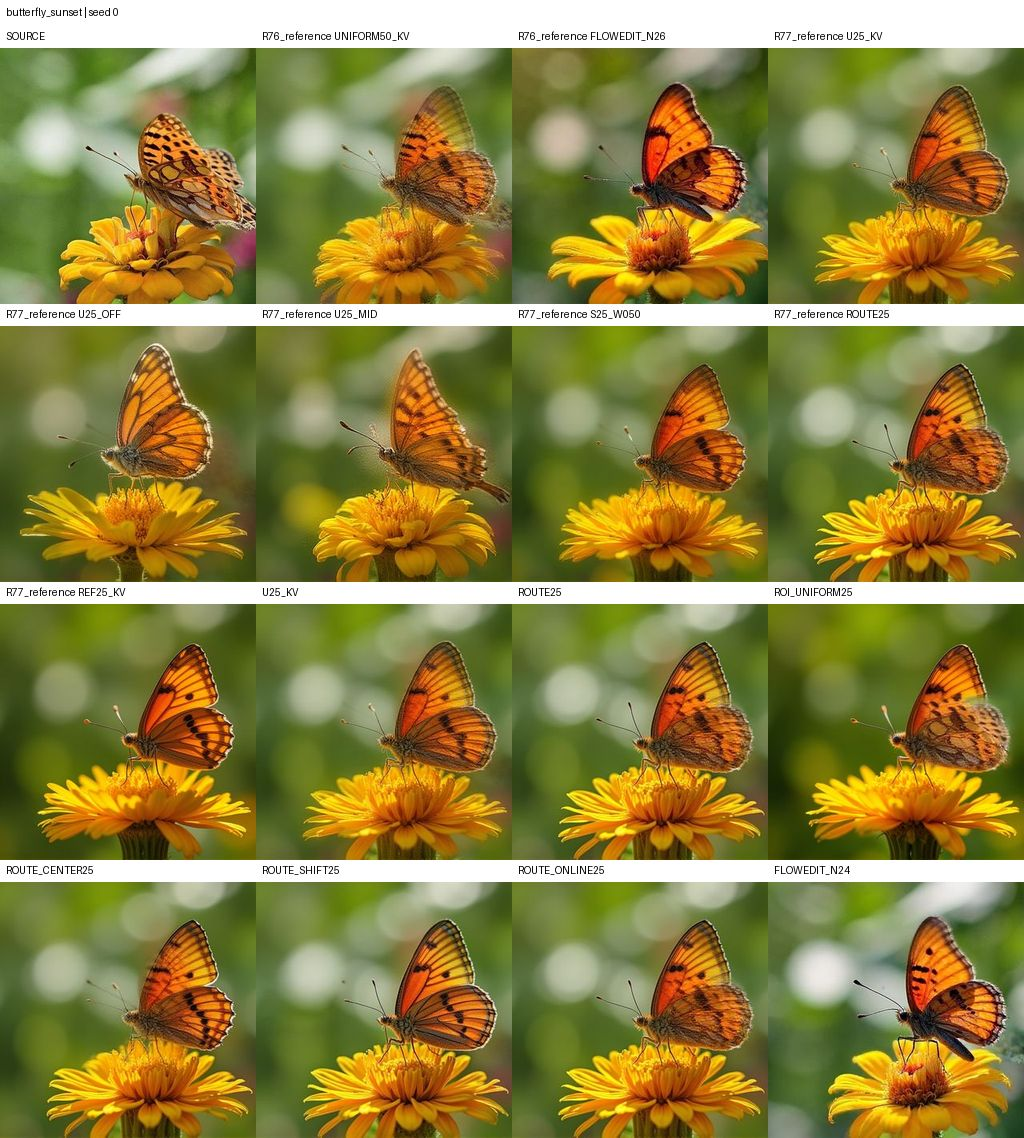
\includegraphics[width=0.90\textwidth,height=0.85\textheight,keepaspectratio]{figures/appendix/r78_butterfly_sunset_s0.jpg}
\caption{Complete recorded comparison sheet: archive R78, butterfly\_sunset\_s0. Cells labeled reference are historical context; only unlabeled current-round arms enter that archive's quantitative table.}
\end{figure}
\clearpage
\begin{figure}[p]
\centering
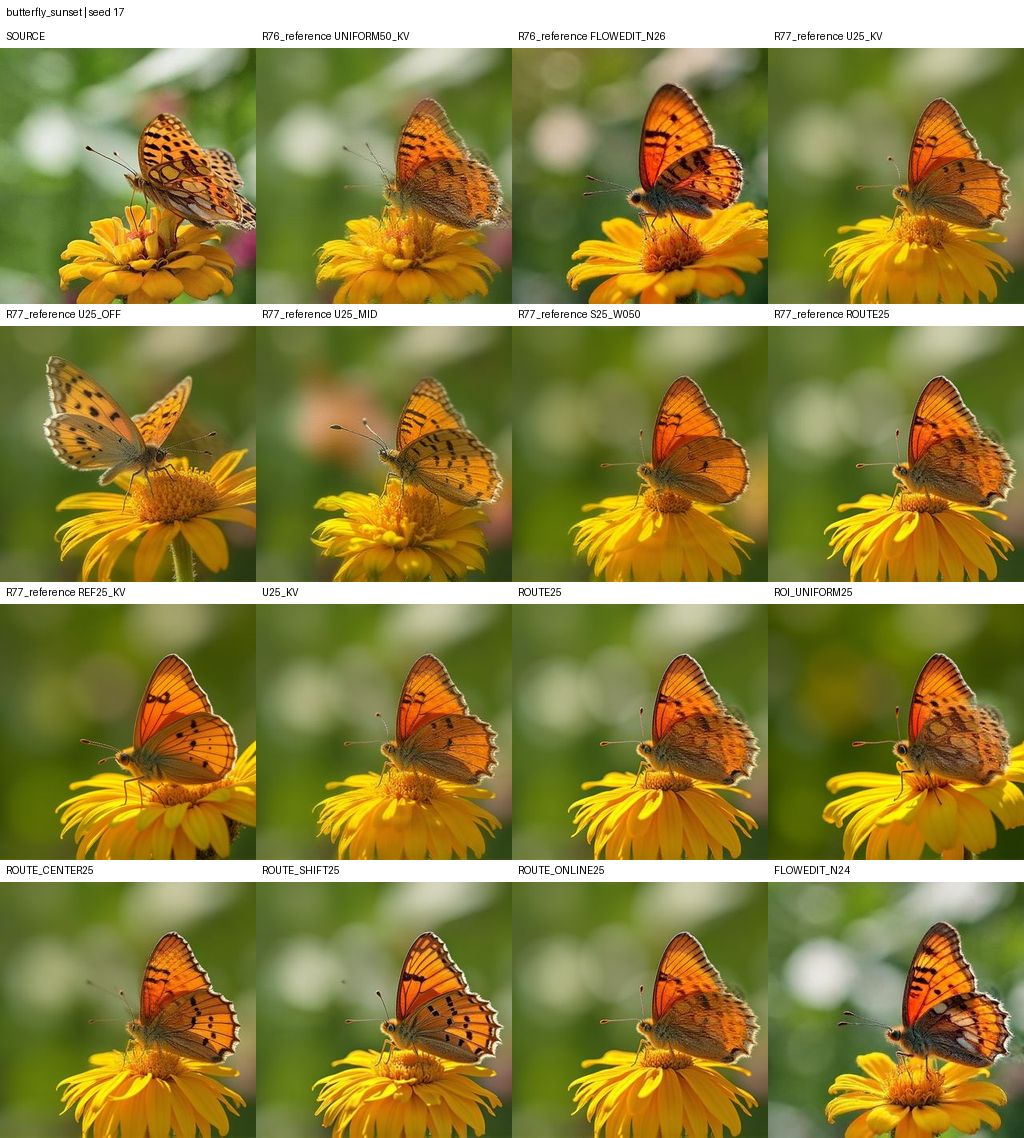
\includegraphics[width=0.90\textwidth,height=0.85\textheight,keepaspectratio]{figures/appendix/r78_butterfly_sunset_s17.jpg}
\caption{Complete recorded comparison sheet: archive R78, butterfly\_sunset\_s17. Cells labeled reference are historical context; only unlabeled current-round arms enter that archive's quantitative table.}
\end{figure}
\clearpage
\begin{figure}[p]
\centering
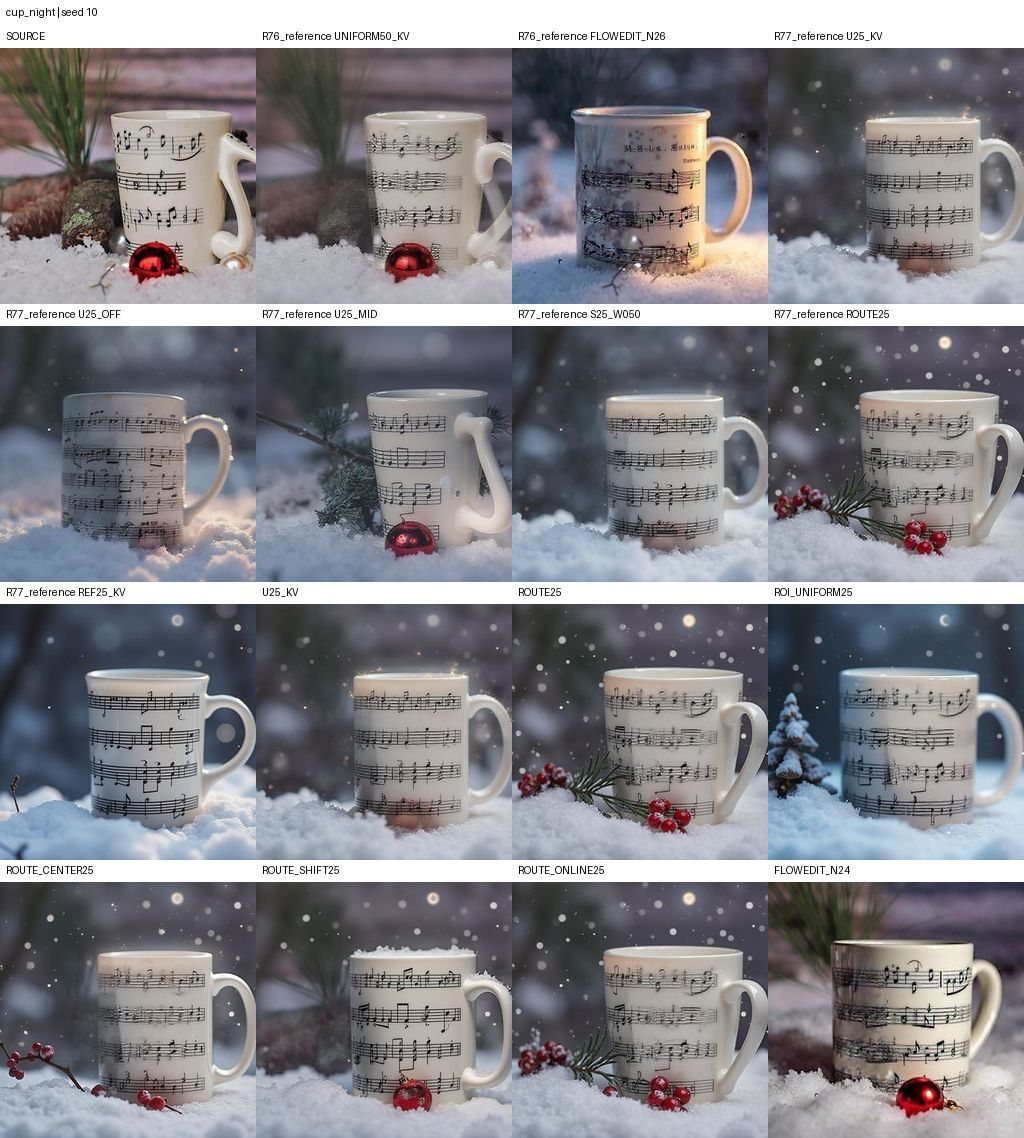
\includegraphics[width=0.90\textwidth,height=0.85\textheight,keepaspectratio]{figures/appendix/r78_cup_night_s10.jpg}
\caption{Complete recorded comparison sheet: archive R78, cup\_night\_s10. Cells labeled reference are historical context; only unlabeled current-round arms enter that archive's quantitative table.}
\end{figure}
\clearpage
\begin{figure}[p]
\centering
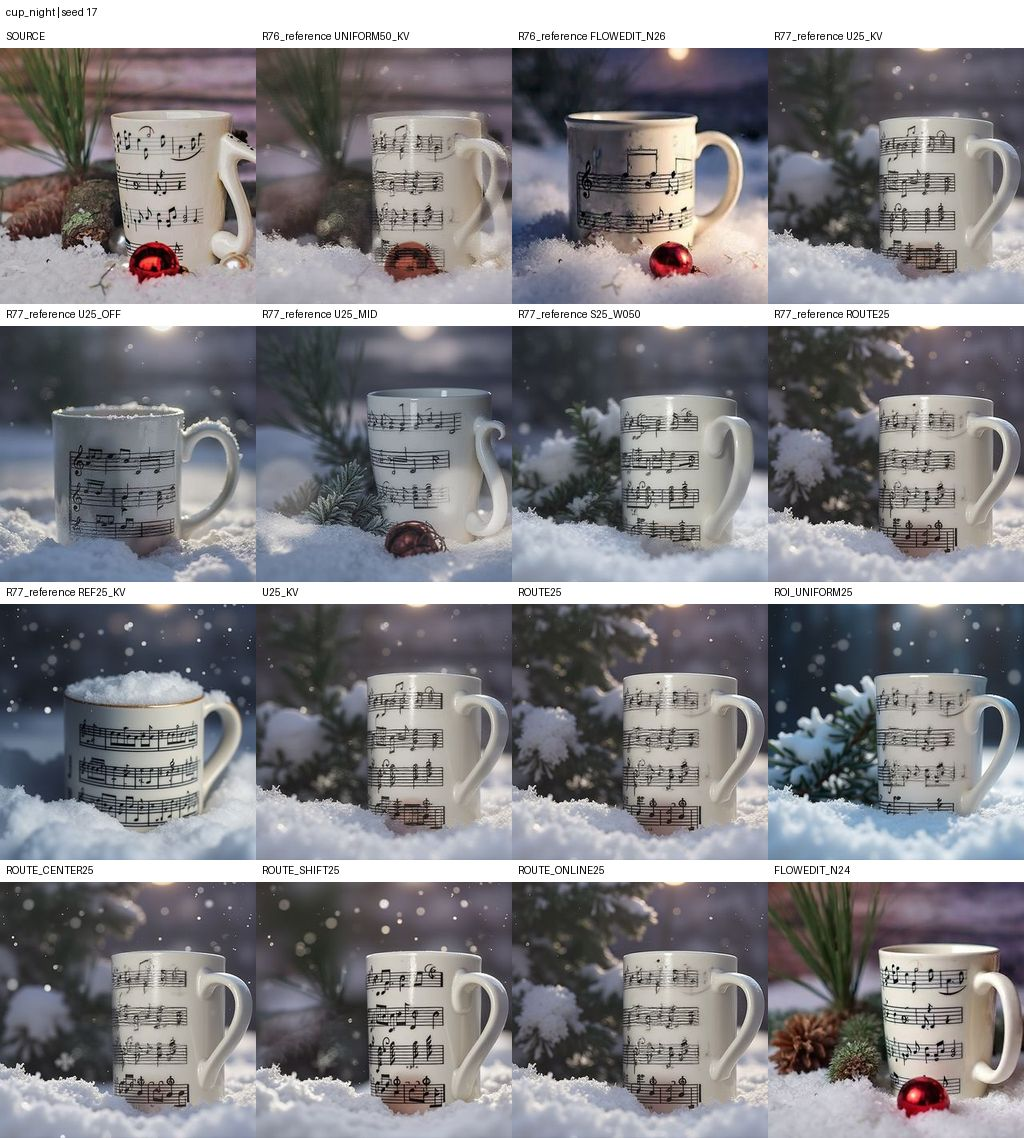
\includegraphics[width=0.90\textwidth,height=0.85\textheight,keepaspectratio]{figures/appendix/r78_cup_night_s17.jpg}
\caption{Complete recorded comparison sheet: archive R78, cup\_night\_s17. Cells labeled reference are historical context; only unlabeled current-round arms enter that archive's quantitative table.}
\end{figure}
\clearpage
\begin{figure}[p]
\centering
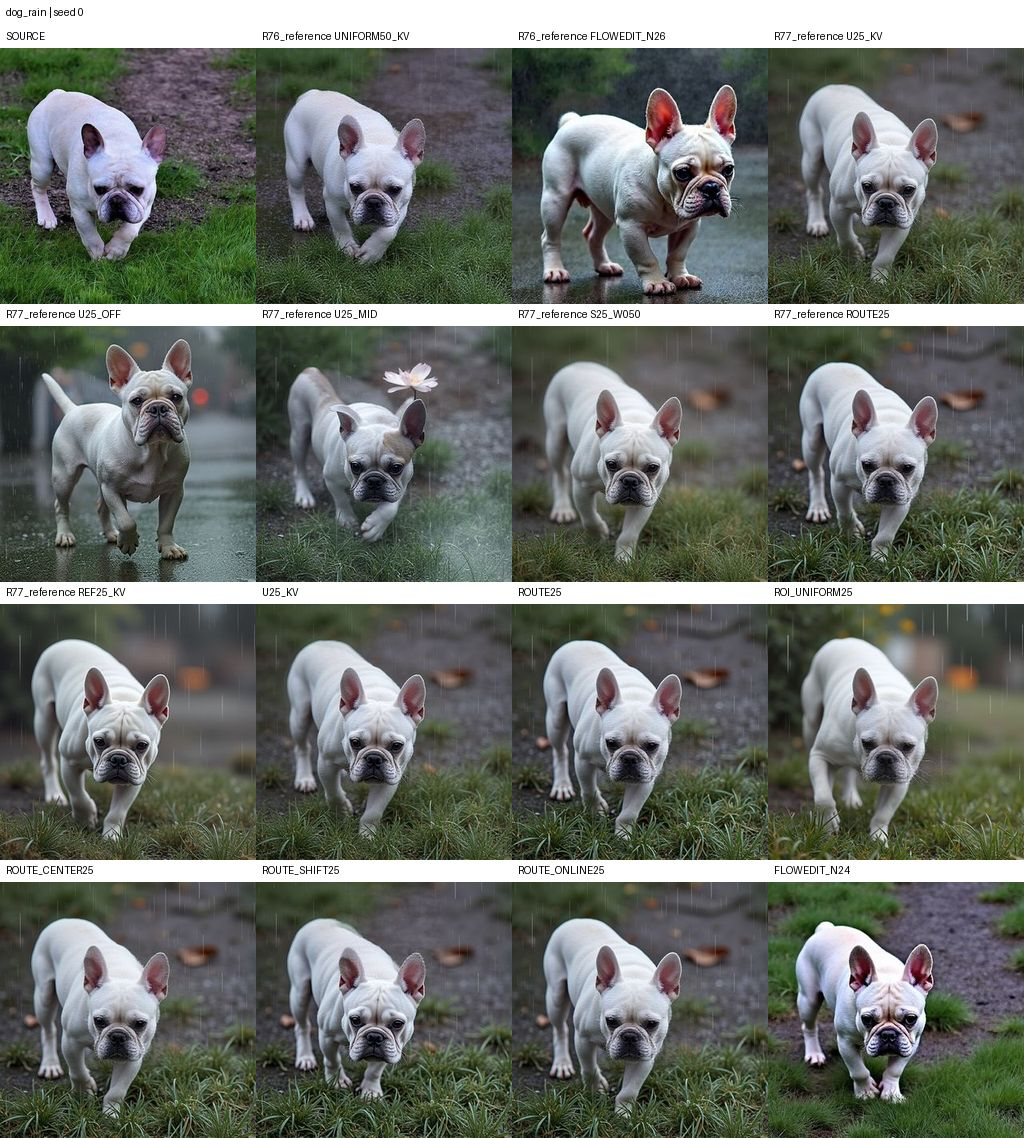
\includegraphics[width=0.90\textwidth,height=0.85\textheight,keepaspectratio]{figures/appendix/r78_dog_rain_s0.jpg}
\caption{Complete recorded comparison sheet: archive R78, dog\_rain\_s0. Cells labeled reference are historical context; only unlabeled current-round arms enter that archive's quantitative table.}
\end{figure}
\clearpage
\begin{figure}[p]
\centering
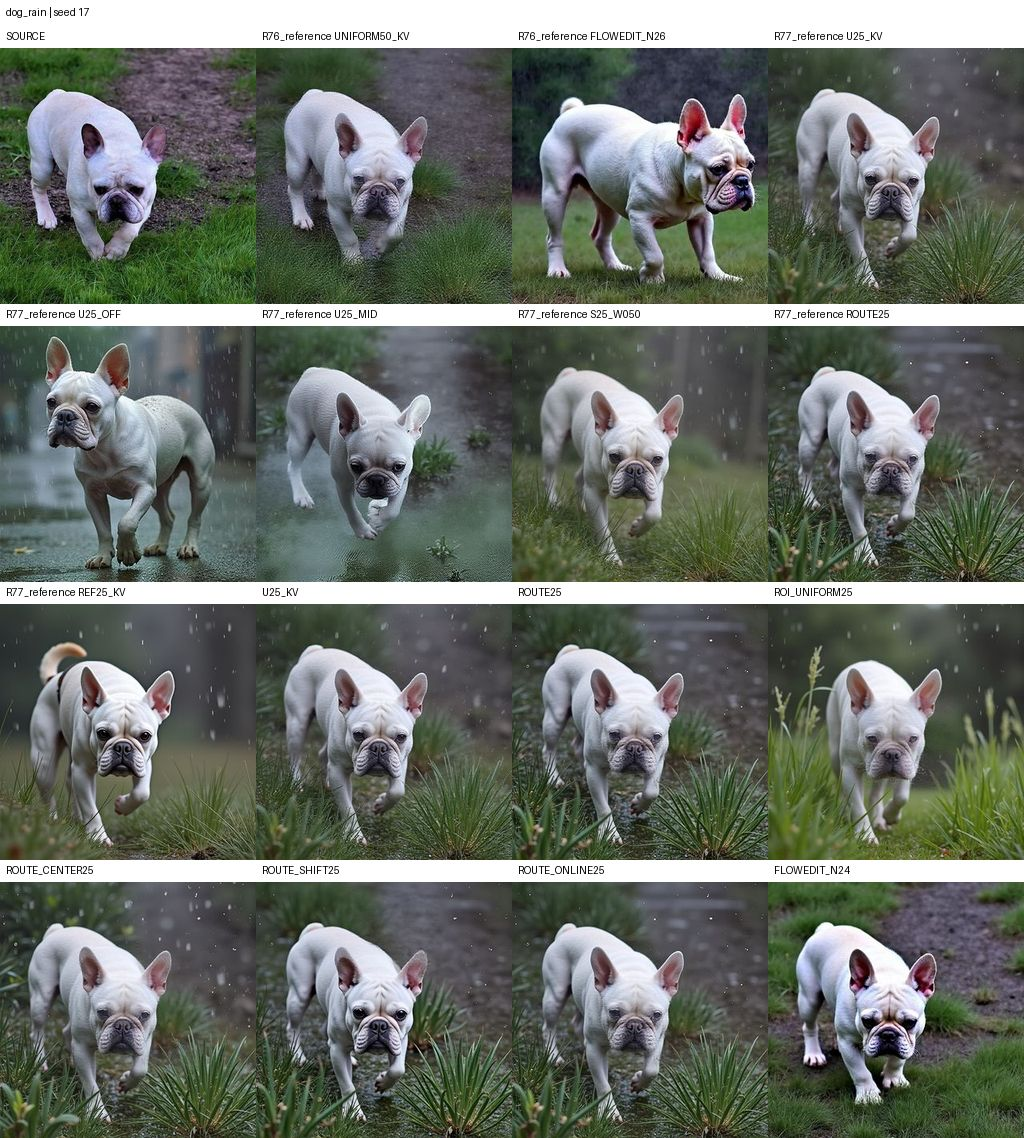
\includegraphics[width=0.90\textwidth,height=0.85\textheight,keepaspectratio]{figures/appendix/r78_dog_rain_s17.jpg}
\caption{Complete recorded comparison sheet: archive R78, dog\_rain\_s17. Cells labeled reference are historical context; only unlabeled current-round arms enter that archive's quantitative table.}
\end{figure}
\clearpage
\begin{figure}[p]
\centering
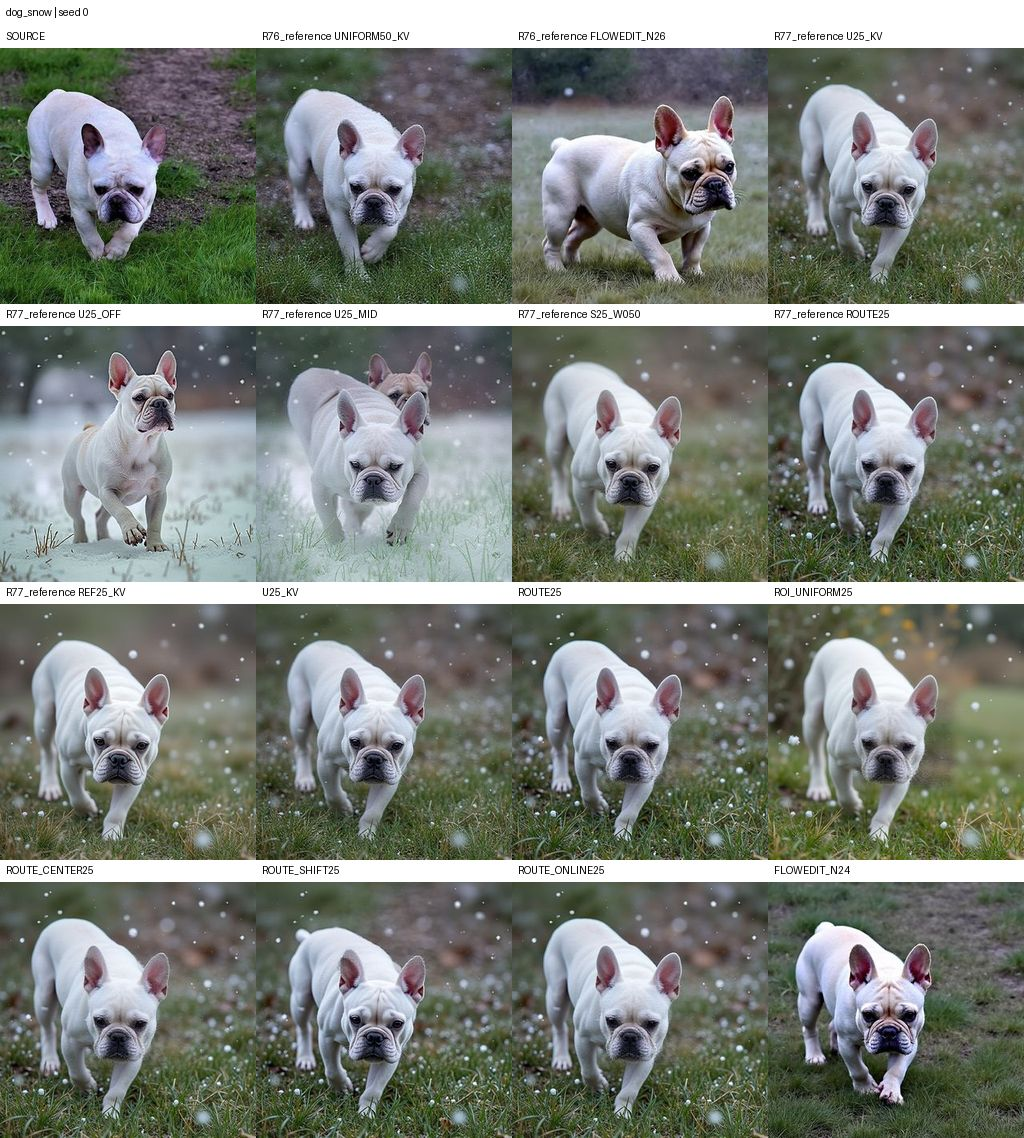
\includegraphics[width=0.90\textwidth,height=0.85\textheight,keepaspectratio]{figures/appendix/r78_dog_snow_s0.jpg}
\caption{Complete recorded comparison sheet: archive R78, dog\_snow\_s0. Cells labeled reference are historical context; only unlabeled current-round arms enter that archive's quantitative table.}
\end{figure}
\clearpage
\begin{figure}[p]
\centering
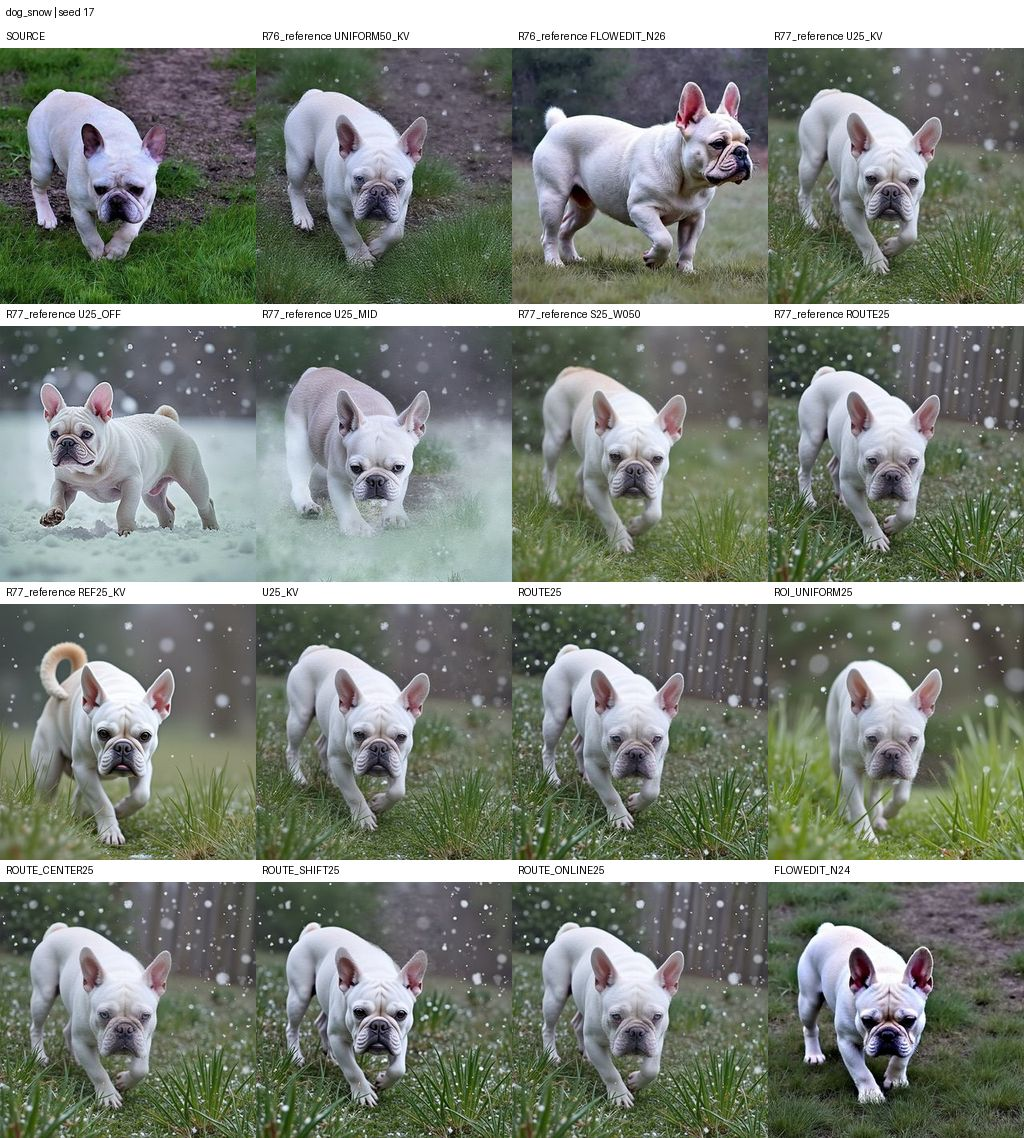
\includegraphics[width=0.90\textwidth,height=0.85\textheight,keepaspectratio]{figures/appendix/r78_dog_snow_s17.jpg}
\caption{Complete recorded comparison sheet: archive R78, dog\_snow\_s17. Cells labeled reference are historical context; only unlabeled current-round arms enter that archive's quantitative table.}
\end{figure}
\clearpage
\begin{figure}[p]
\centering
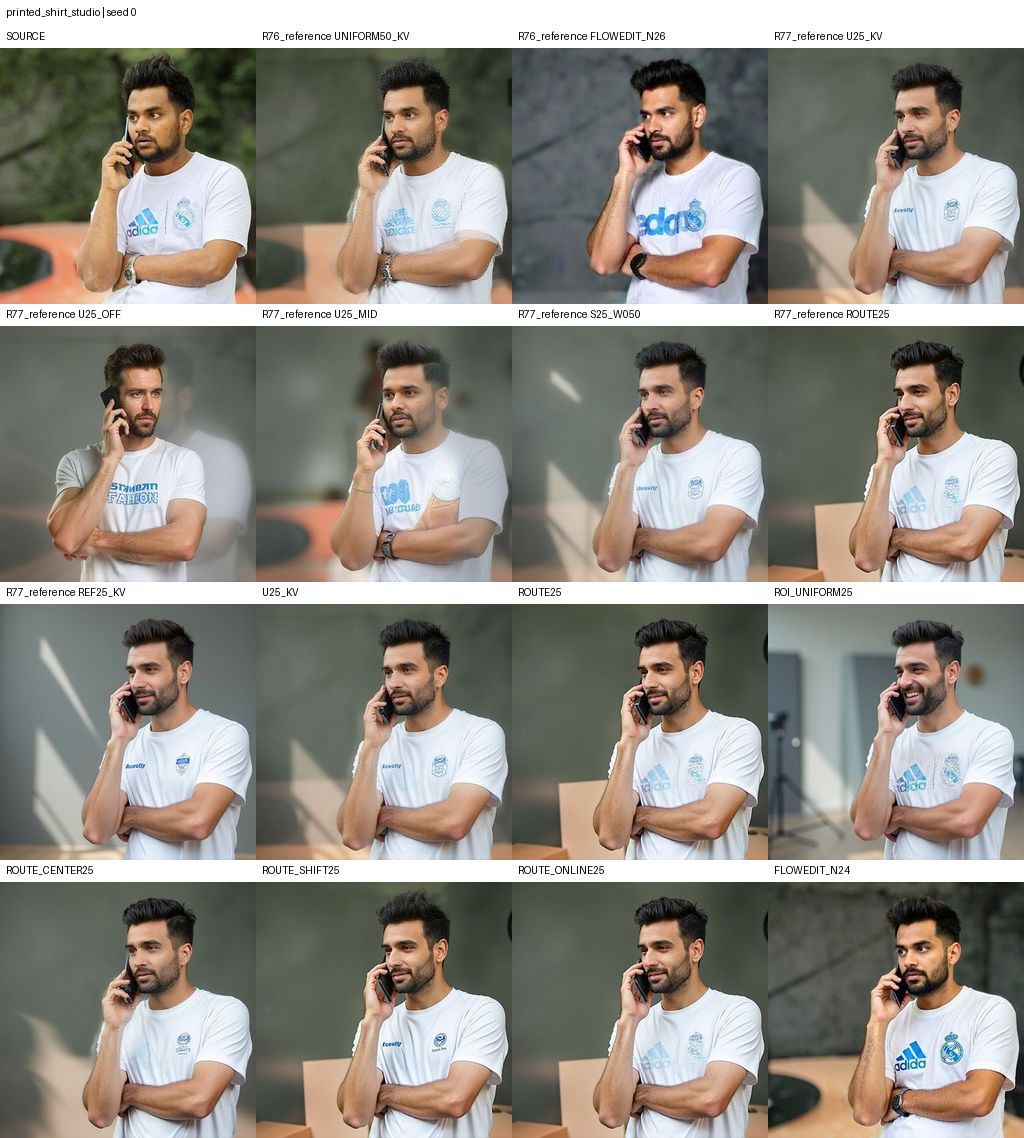
\includegraphics[width=0.90\textwidth,height=0.85\textheight,keepaspectratio]{figures/appendix/r78_printed_shirt_studio_s0.jpg}
\caption{Complete recorded comparison sheet: archive R78, printed\_shirt\_studio\_s0. Cells labeled reference are historical context; only unlabeled current-round arms enter that archive's quantitative table.}
\end{figure}
\clearpage
\begin{figure}[p]
\centering
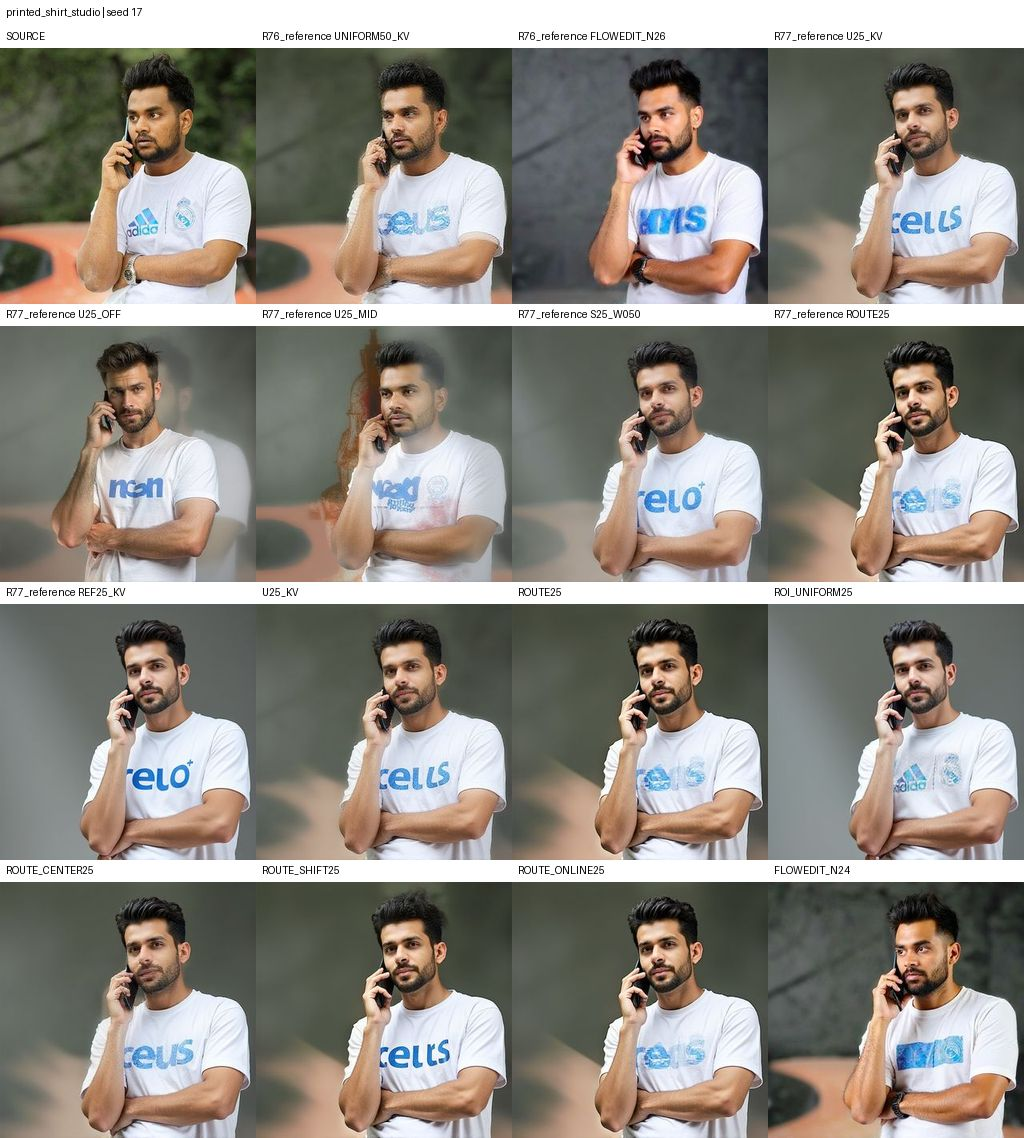
\includegraphics[width=0.90\textwidth,height=0.85\textheight,keepaspectratio]{figures/appendix/r78_printed_shirt_studio_s17.jpg}
\caption{Complete recorded comparison sheet: archive R78, printed\_shirt\_studio\_s17. Cells labeled reference are historical context; only unlabeled current-round arms enter that archive's quantitative table.}
\end{figure}
\clearpage
\begin{figure}[p]
\centering
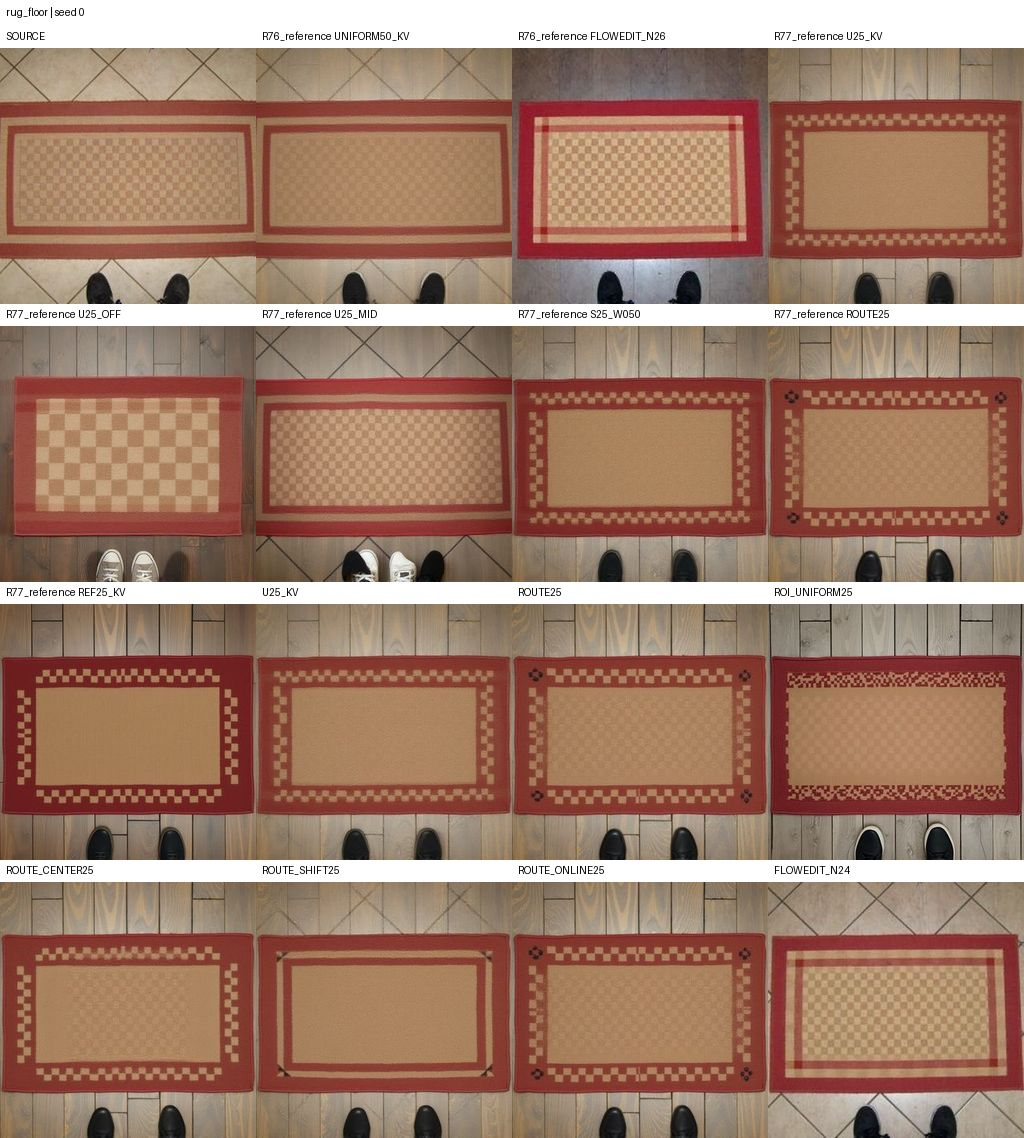
\includegraphics[width=0.90\textwidth,height=0.85\textheight,keepaspectratio]{figures/appendix/r78_rug_floor_s0.jpg}
\caption{Complete recorded comparison sheet: archive R78, rug\_floor\_s0. Cells labeled reference are historical context; only unlabeled current-round arms enter that archive's quantitative table.}
\end{figure}
\clearpage
\begin{figure}[p]
\centering
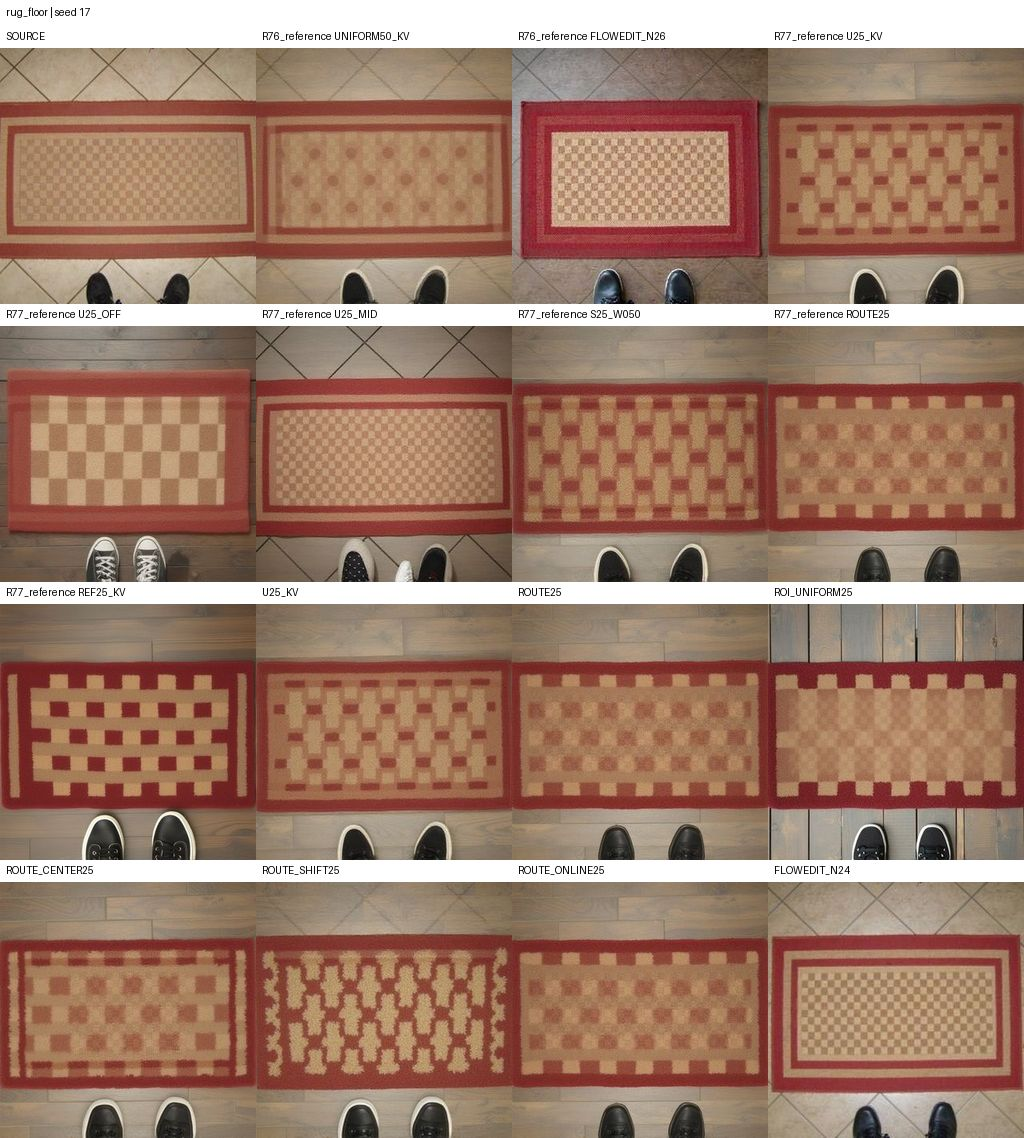
\includegraphics[width=0.90\textwidth,height=0.85\textheight,keepaspectratio]{figures/appendix/r78_rug_floor_s17.jpg}
\caption{Complete recorded comparison sheet: archive R78, rug\_floor\_s17. Cells labeled reference are historical context; only unlabeled current-round arms enter that archive's quantitative table.}
\end{figure}
\clearpage
\begin{figure}[p]
\centering
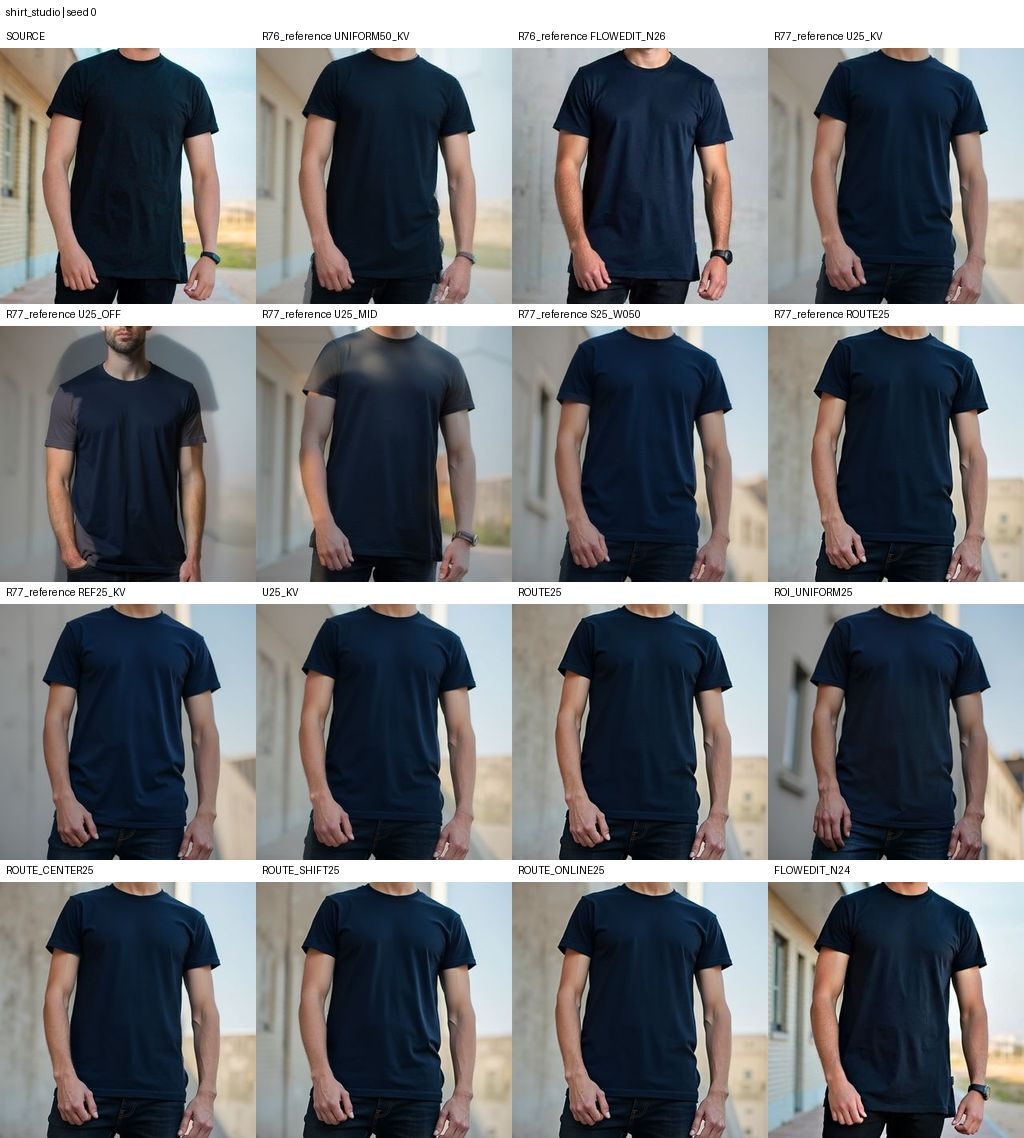
\includegraphics[width=0.90\textwidth,height=0.85\textheight,keepaspectratio]{figures/appendix/r78_shirt_studio_s0.jpg}
\caption{Complete recorded comparison sheet: archive R78, shirt\_studio\_s0. Cells labeled reference are historical context; only unlabeled current-round arms enter that archive's quantitative table.}
\end{figure}
\clearpage
\begin{figure}[p]
\centering
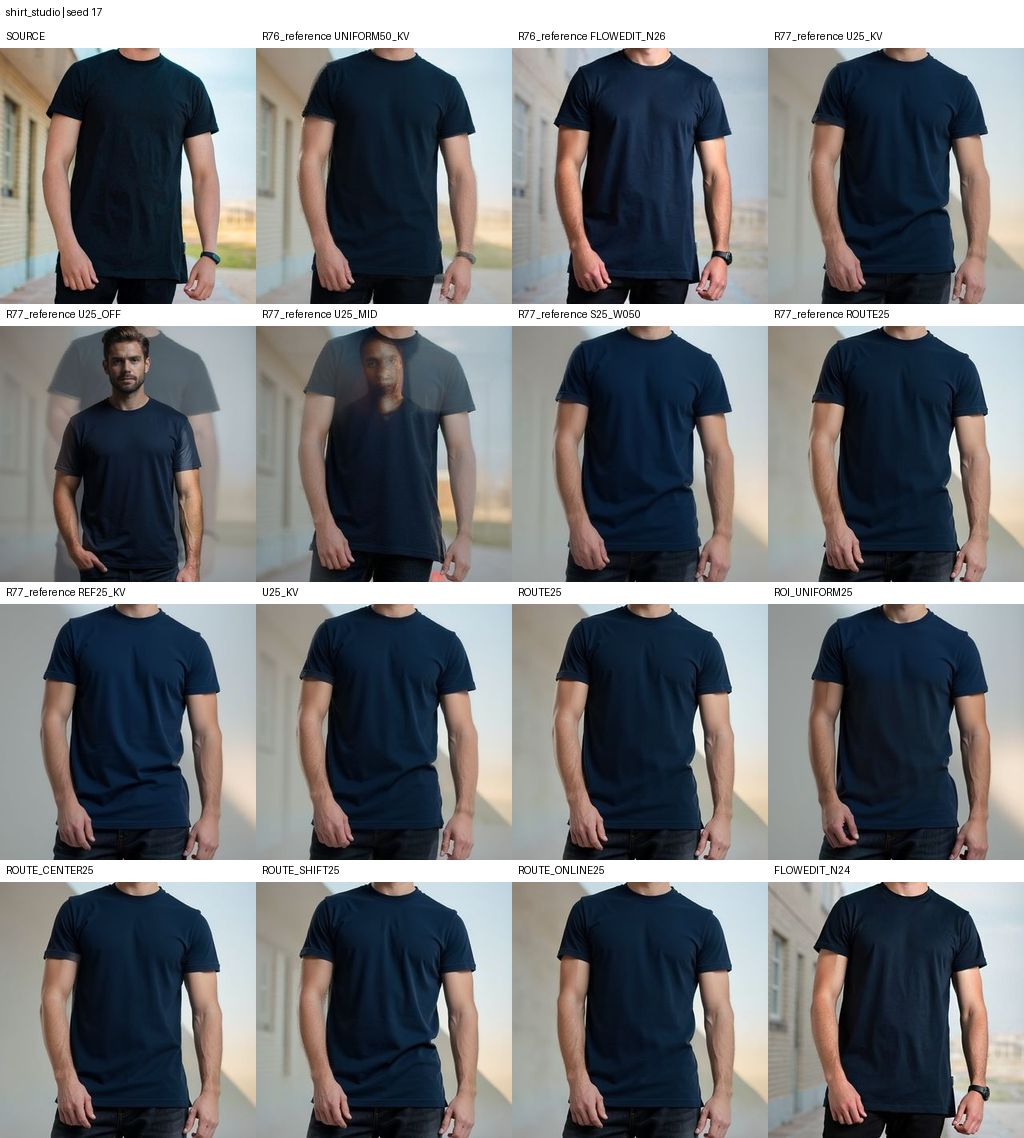
\includegraphics[width=0.90\textwidth,height=0.85\textheight,keepaspectratio]{figures/appendix/r78_shirt_studio_s17.jpg}
\caption{Complete recorded comparison sheet: archive R78, shirt\_studio\_s17. Cells labeled reference are historical context; only unlabeled current-round arms enter that archive's quantitative table.}
\end{figure}
\clearpage
\begin{figure}[p]
\centering
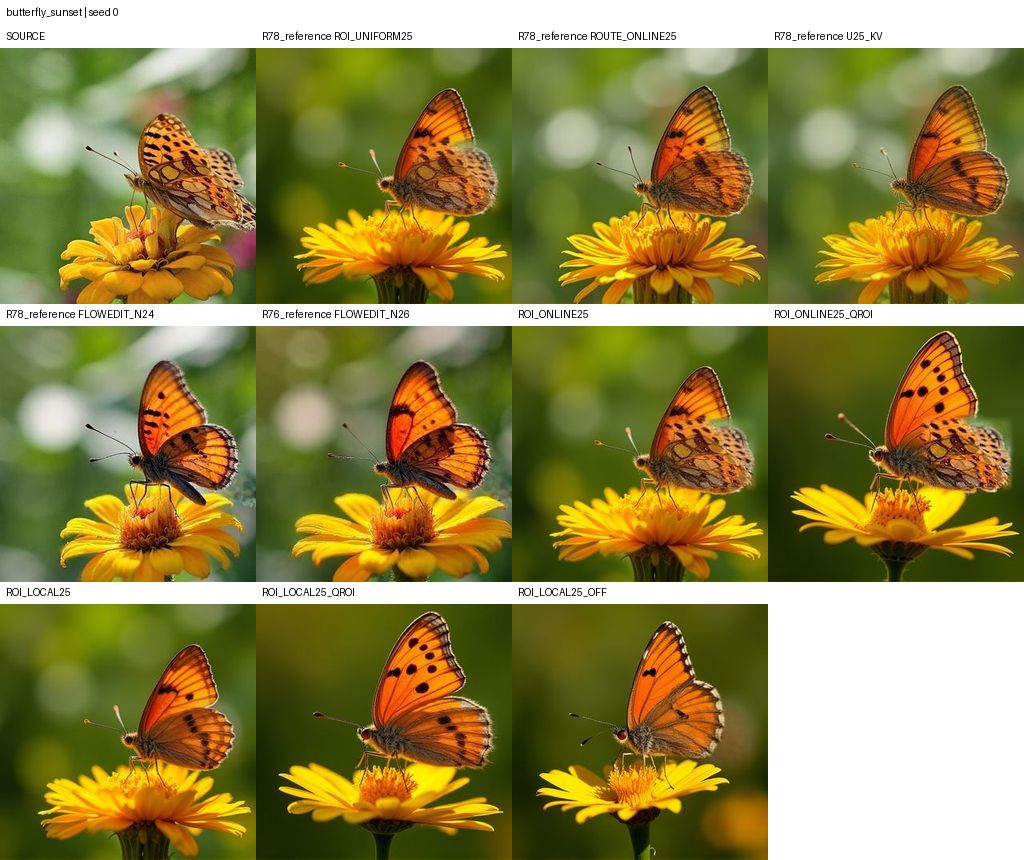
\includegraphics[width=0.90\textwidth,height=0.85\textheight,keepaspectratio]{figures/appendix/r79_butterfly_sunset_s0.jpg}
\caption{Complete recorded comparison sheet: archive R79, butterfly\_sunset\_s0. Cells labeled reference are historical context; only unlabeled current-round arms enter that archive's quantitative table.}
\end{figure}
\clearpage
\begin{figure}[p]
\centering
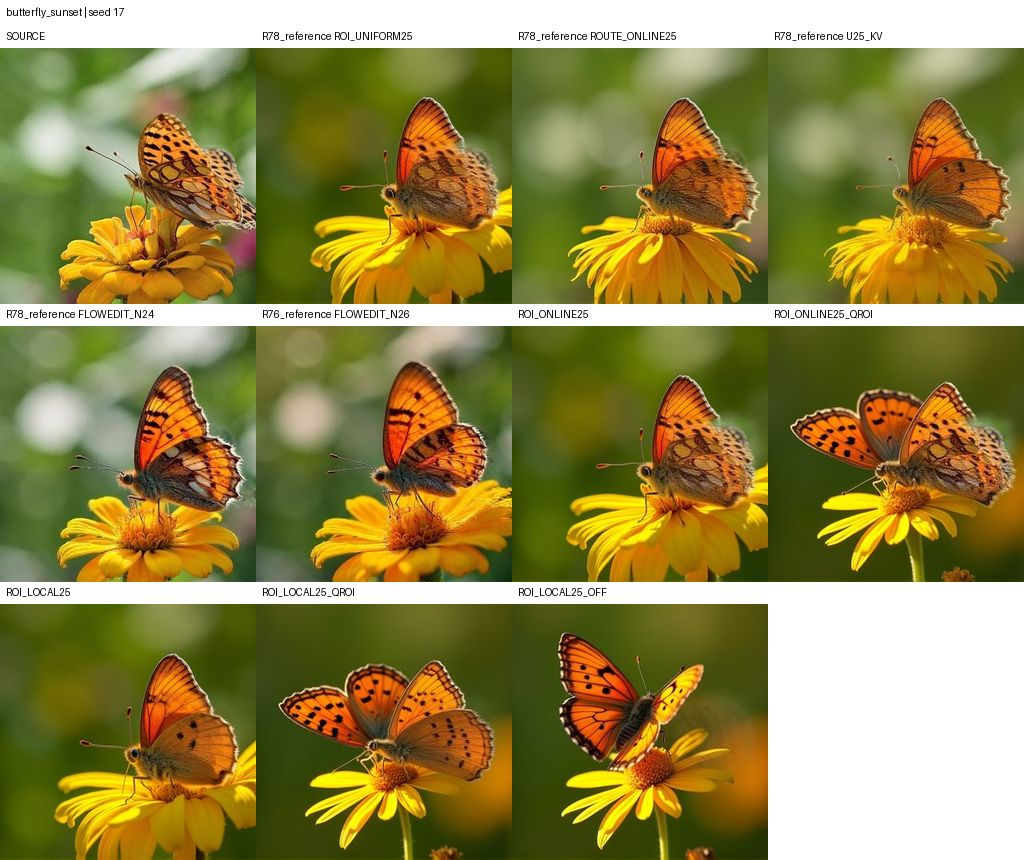
\includegraphics[width=0.90\textwidth,height=0.85\textheight,keepaspectratio]{figures/appendix/r79_butterfly_sunset_s17.jpg}
\caption{Complete recorded comparison sheet: archive R79, butterfly\_sunset\_s17. Cells labeled reference are historical context; only unlabeled current-round arms enter that archive's quantitative table.}
\end{figure}
\clearpage
\begin{figure}[p]
\centering
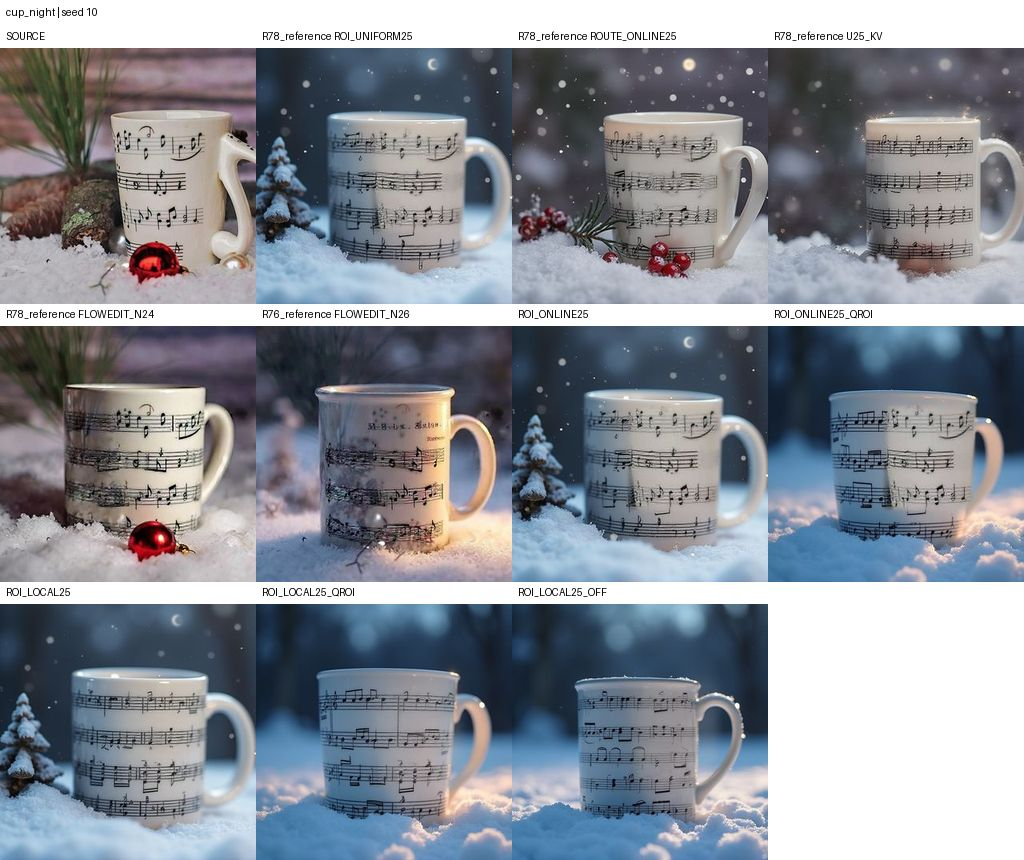
\includegraphics[width=0.90\textwidth,height=0.85\textheight,keepaspectratio]{figures/appendix/r79_cup_night_s10.jpg}
\caption{Complete recorded comparison sheet: archive R79, cup\_night\_s10. Cells labeled reference are historical context; only unlabeled current-round arms enter that archive's quantitative table.}
\end{figure}
\clearpage
\begin{figure}[p]
\centering
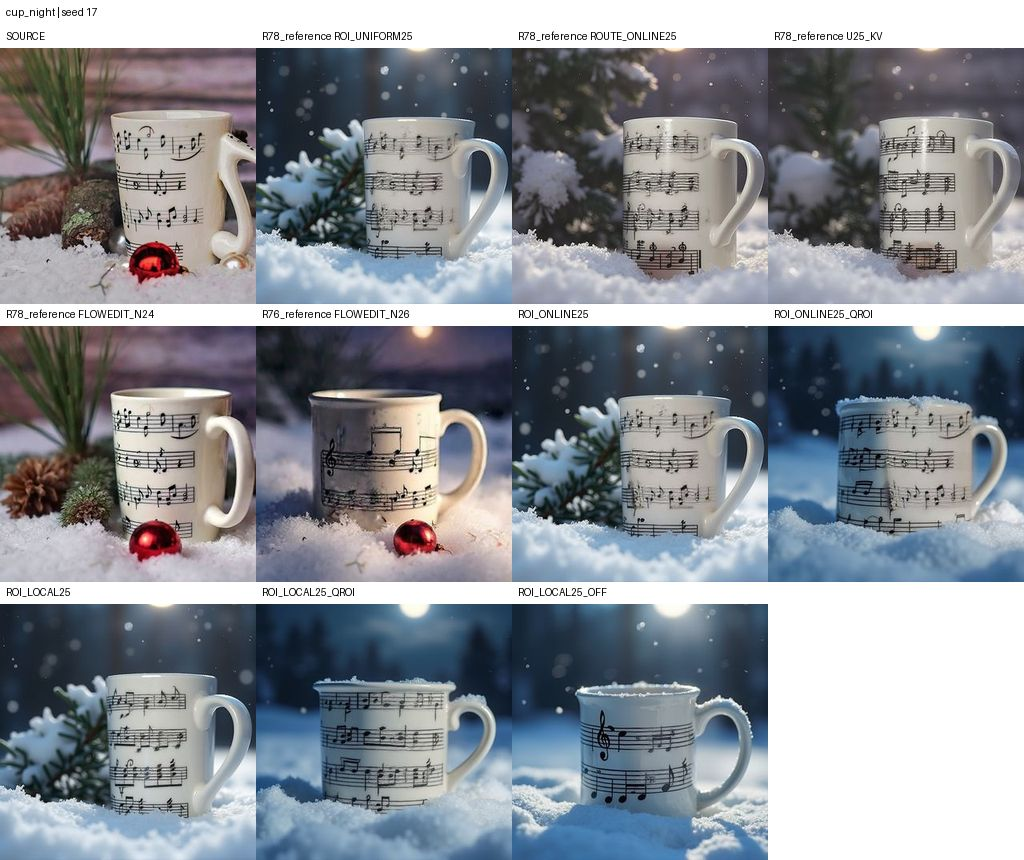
\includegraphics[width=0.90\textwidth,height=0.85\textheight,keepaspectratio]{figures/appendix/r79_cup_night_s17.jpg}
\caption{Complete recorded comparison sheet: archive R79, cup\_night\_s17. Cells labeled reference are historical context; only unlabeled current-round arms enter that archive's quantitative table.}
\end{figure}
\clearpage
\begin{figure}[p]
\centering
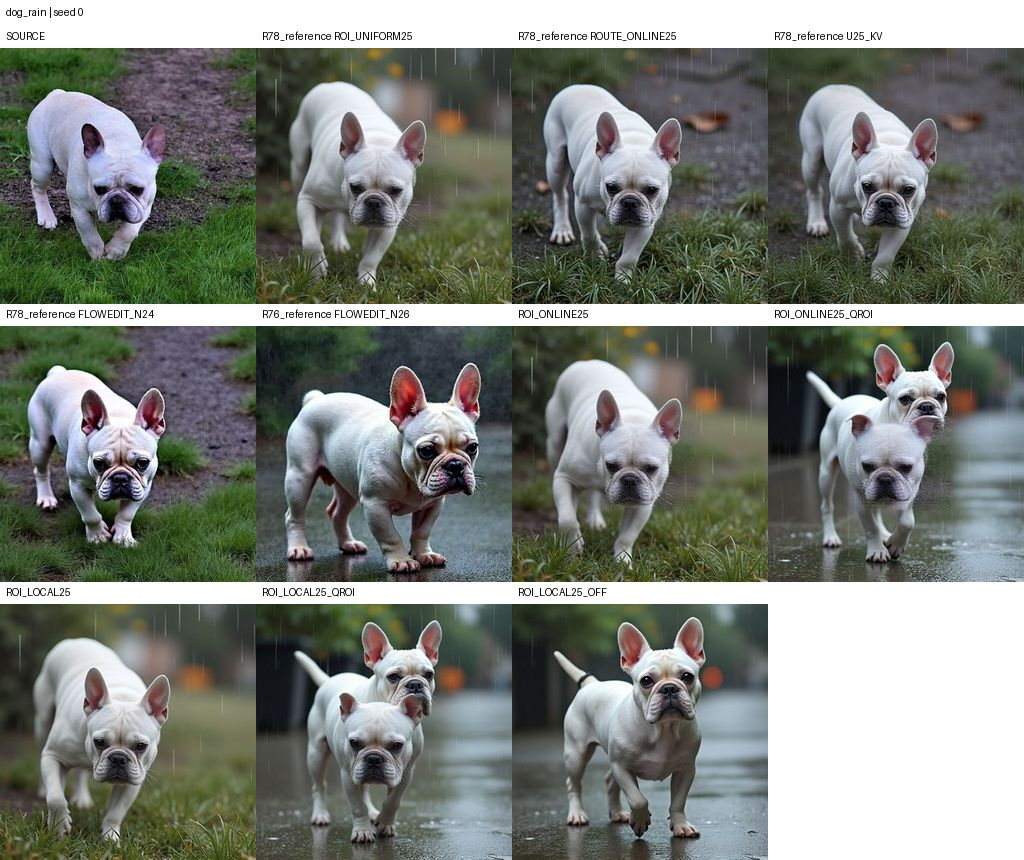
\includegraphics[width=0.90\textwidth,height=0.85\textheight,keepaspectratio]{figures/appendix/r79_dog_rain_s0.jpg}
\caption{Complete recorded comparison sheet: archive R79, dog\_rain\_s0. Cells labeled reference are historical context; only unlabeled current-round arms enter that archive's quantitative table.}
\end{figure}
\clearpage
\begin{figure}[p]
\centering
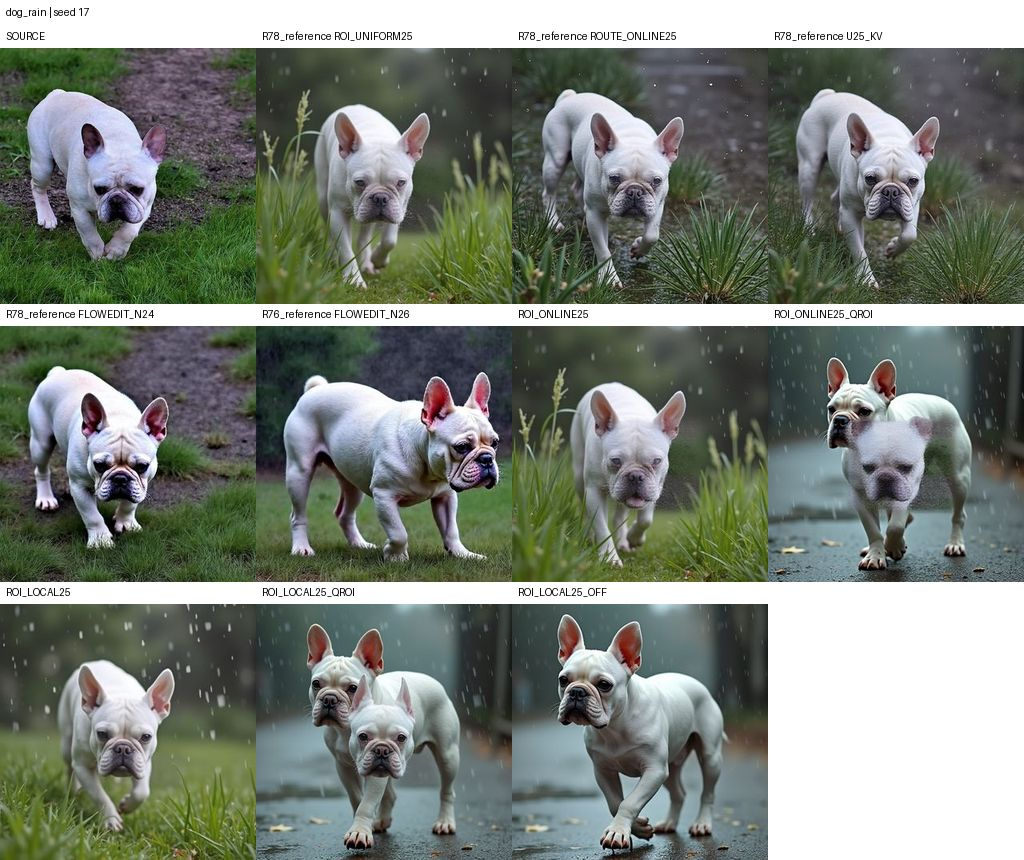
\includegraphics[width=0.90\textwidth,height=0.85\textheight,keepaspectratio]{figures/appendix/r79_dog_rain_s17.jpg}
\caption{Complete recorded comparison sheet: archive R79, dog\_rain\_s17. Cells labeled reference are historical context; only unlabeled current-round arms enter that archive's quantitative table.}
\end{figure}
\clearpage
\begin{figure}[p]
\centering
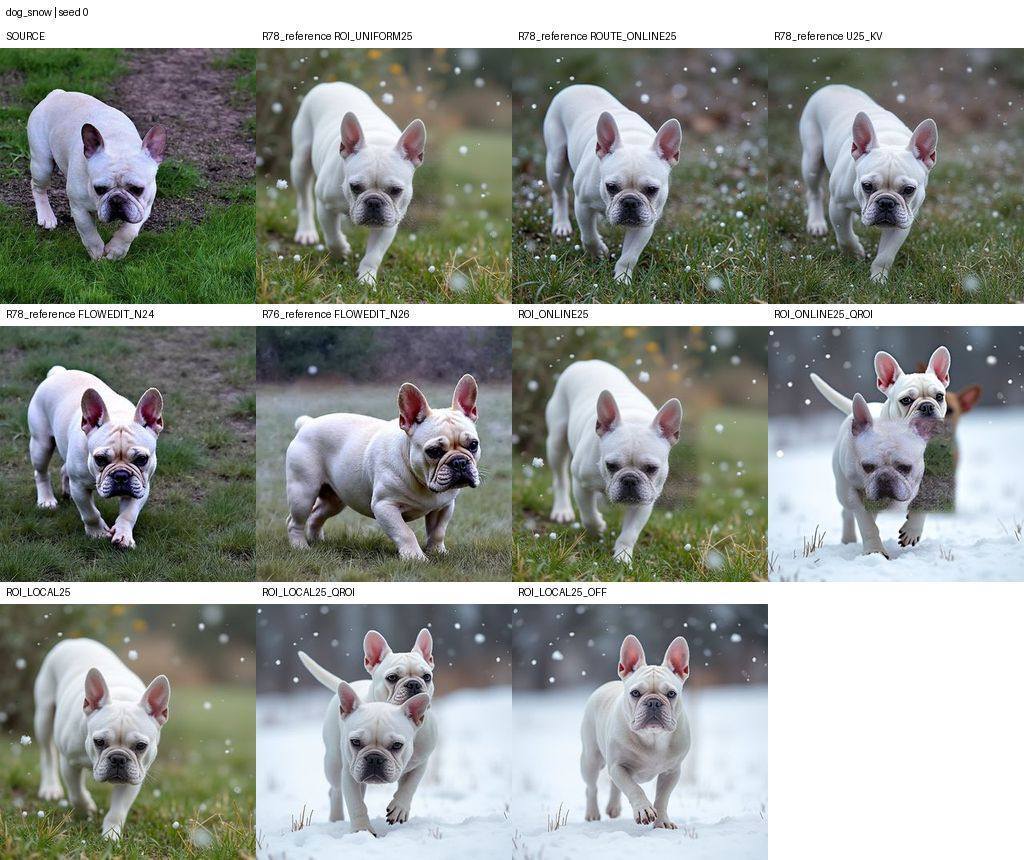
\includegraphics[width=0.90\textwidth,height=0.85\textheight,keepaspectratio]{figures/appendix/r79_dog_snow_s0.jpg}
\caption{Complete recorded comparison sheet: archive R79, dog\_snow\_s0. Cells labeled reference are historical context; only unlabeled current-round arms enter that archive's quantitative table.}
\end{figure}
\clearpage
\begin{figure}[p]
\centering
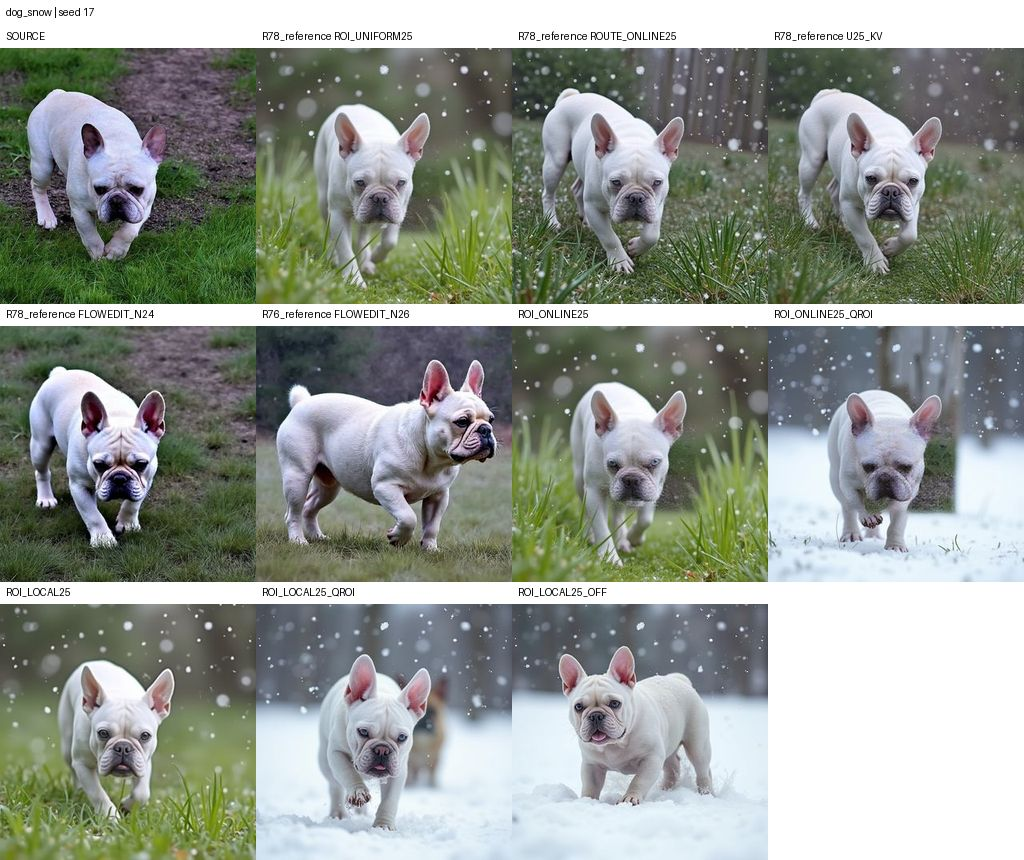
\includegraphics[width=0.90\textwidth,height=0.85\textheight,keepaspectratio]{figures/appendix/r79_dog_snow_s17.jpg}
\caption{Complete recorded comparison sheet: archive R79, dog\_snow\_s17. Cells labeled reference are historical context; only unlabeled current-round arms enter that archive's quantitative table.}
\end{figure}
\clearpage
\begin{figure}[p]
\centering
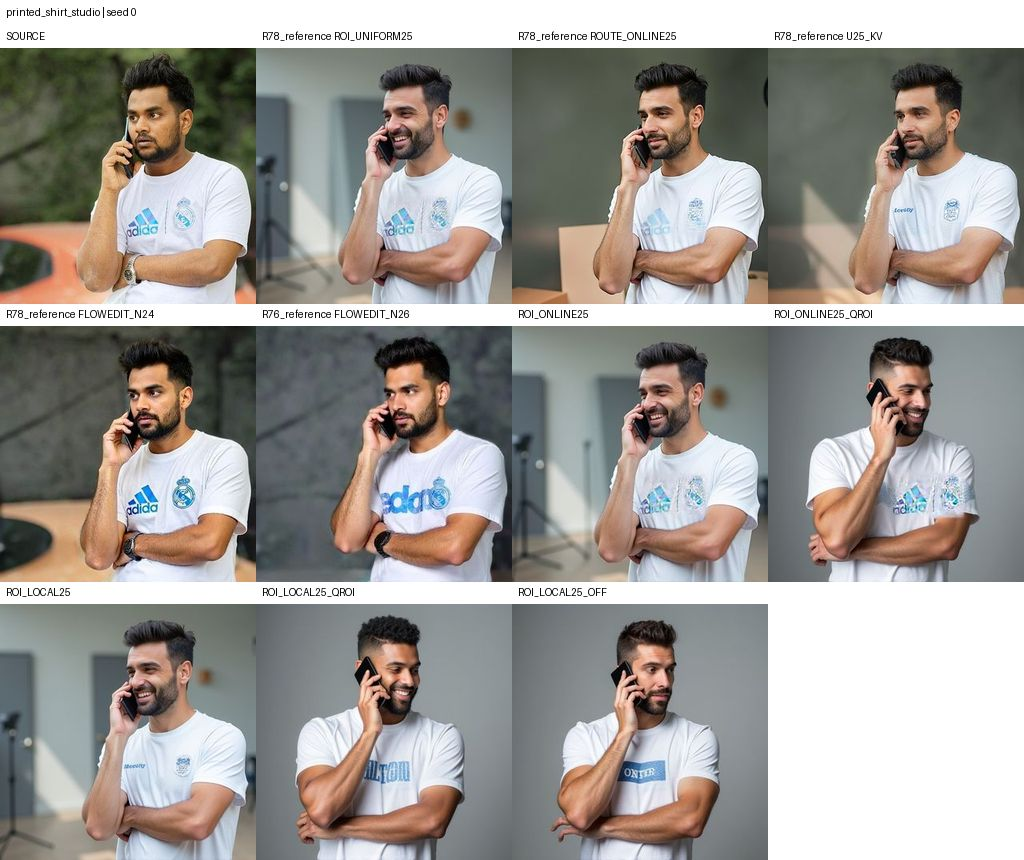
\includegraphics[width=0.90\textwidth,height=0.85\textheight,keepaspectratio]{figures/appendix/r79_printed_shirt_studio_s0.jpg}
\caption{Complete recorded comparison sheet: archive R79, printed\_shirt\_studio\_s0. Cells labeled reference are historical context; only unlabeled current-round arms enter that archive's quantitative table.}
\end{figure}
\clearpage
\begin{figure}[p]
\centering
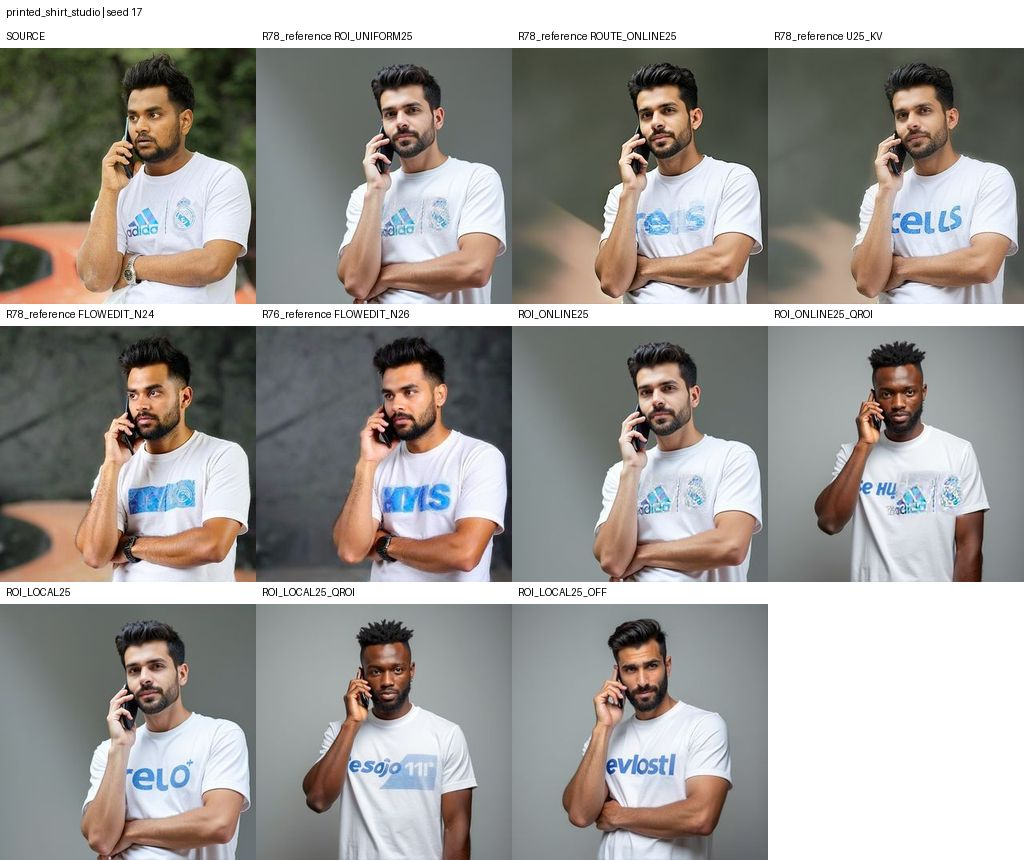
\includegraphics[width=0.90\textwidth,height=0.85\textheight,keepaspectratio]{figures/appendix/r79_printed_shirt_studio_s17.jpg}
\caption{Complete recorded comparison sheet: archive R79, printed\_shirt\_studio\_s17. Cells labeled reference are historical context; only unlabeled current-round arms enter that archive's quantitative table.}
\end{figure}
\clearpage
\begin{figure}[p]
\centering
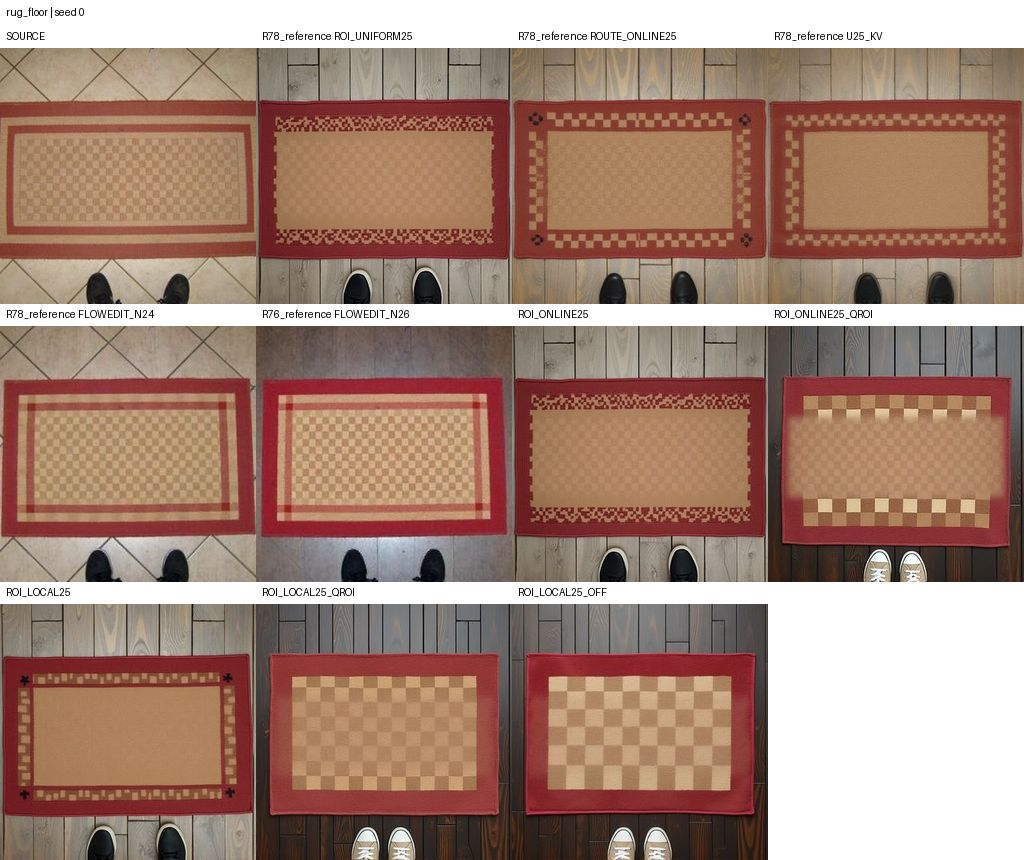
\includegraphics[width=0.90\textwidth,height=0.85\textheight,keepaspectratio]{figures/appendix/r79_rug_floor_s0.jpg}
\caption{Complete recorded comparison sheet: archive R79, rug\_floor\_s0. Cells labeled reference are historical context; only unlabeled current-round arms enter that archive's quantitative table.}
\end{figure}
\clearpage
\begin{figure}[p]
\centering
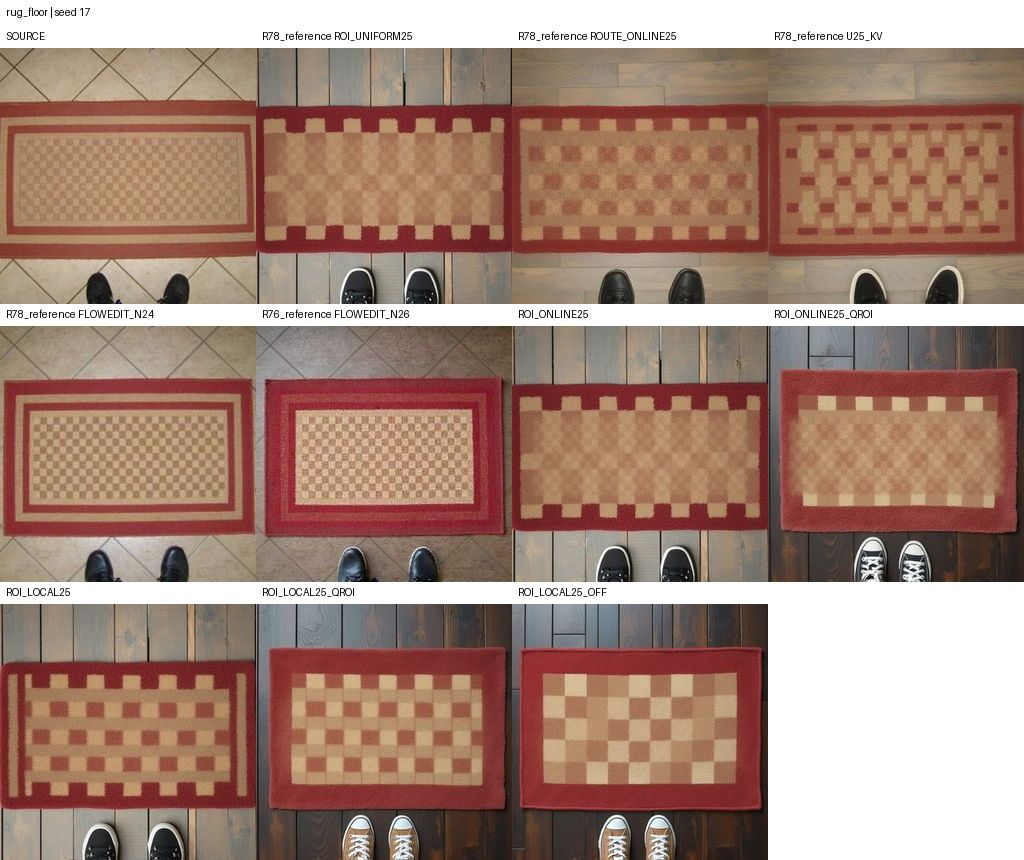
\includegraphics[width=0.90\textwidth,height=0.85\textheight,keepaspectratio]{figures/appendix/r79_rug_floor_s17.jpg}
\caption{Complete recorded comparison sheet: archive R79, rug\_floor\_s17. Cells labeled reference are historical context; only unlabeled current-round arms enter that archive's quantitative table.}
\end{figure}
\clearpage
\begin{figure}[p]
\centering
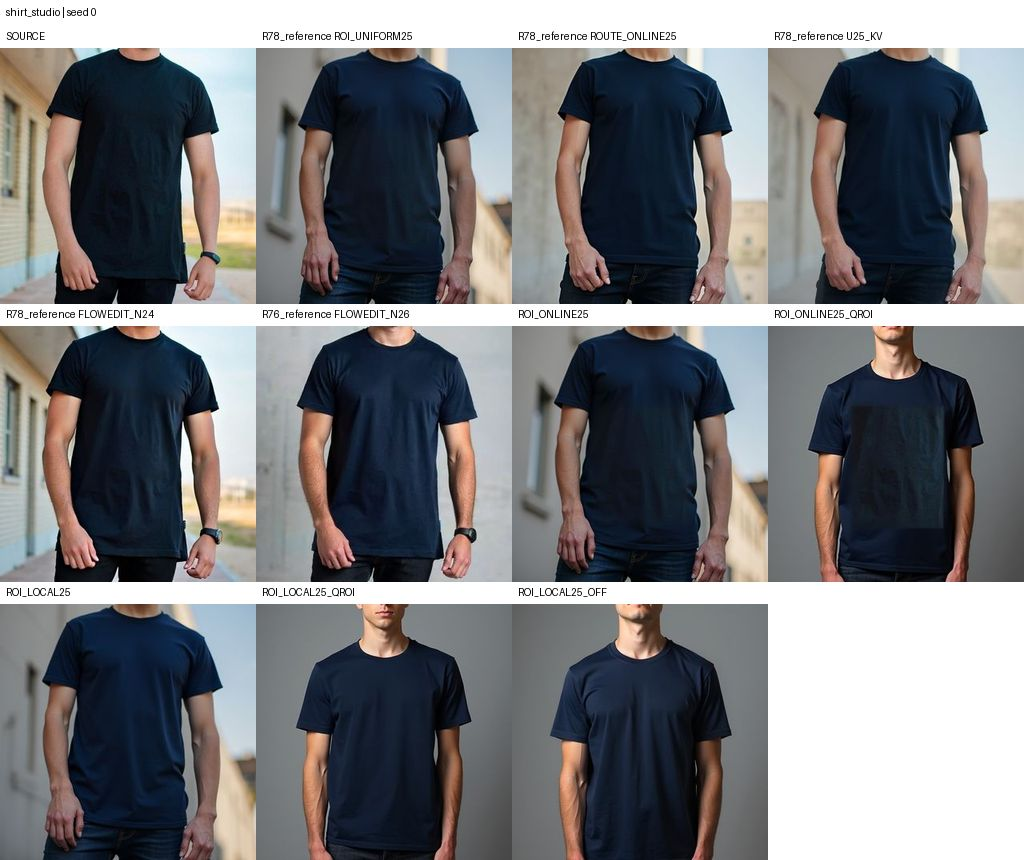
\includegraphics[width=0.90\textwidth,height=0.85\textheight,keepaspectratio]{figures/appendix/r79_shirt_studio_s0.jpg}
\caption{Complete recorded comparison sheet: archive R79, shirt\_studio\_s0. Cells labeled reference are historical context; only unlabeled current-round arms enter that archive's quantitative table.}
\end{figure}
\clearpage
\begin{figure}[p]
\centering
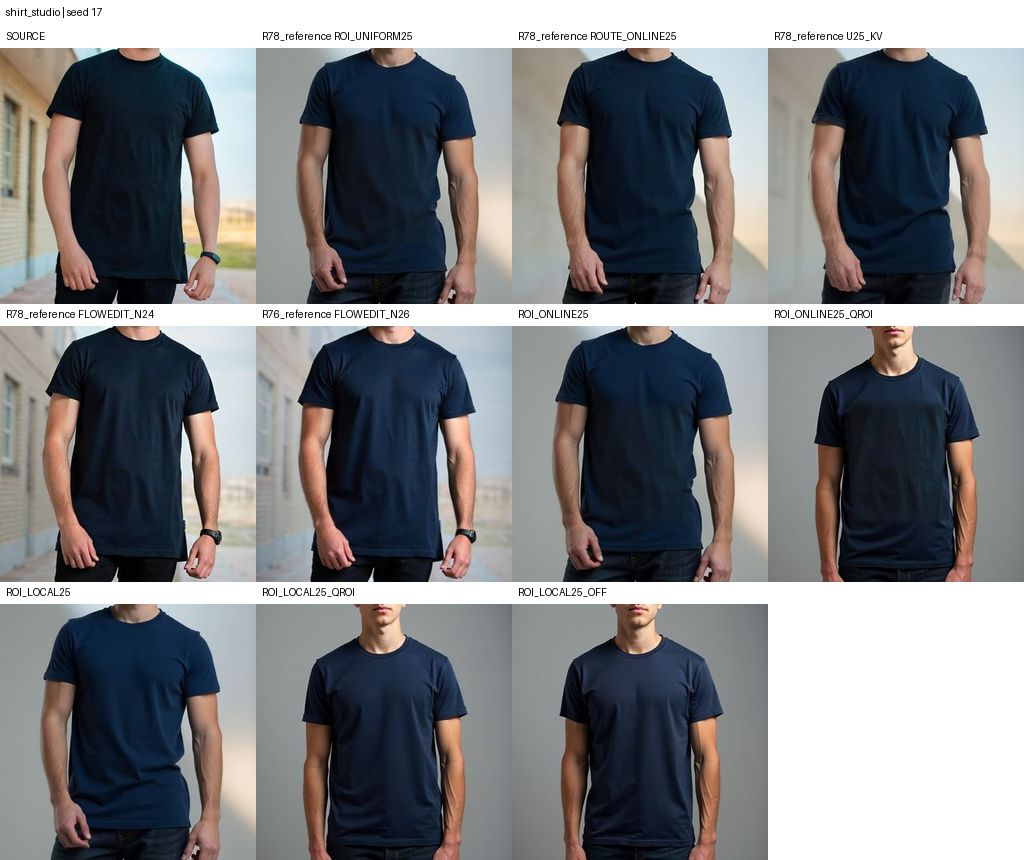
\includegraphics[width=0.90\textwidth,height=0.85\textheight,keepaspectratio]{figures/appendix/r79_shirt_studio_s17.jpg}
\caption{Complete recorded comparison sheet: archive R79, shirt\_studio\_s17. Cells labeled reference are historical context; only unlabeled current-round arms enter that archive's quantitative table.}
\end{figure}

\end{document}
